\pdfoutput=1
\documentclass[10pt,journal,letterpaper,twoside,compsoc]{IEEEtran}

%%%%%%%%%%%%%%%%%%%%%%%%%%%%%%%%%%%%%%%%%%%%%%%%%%%%%%%%%%%
% Packages
%%%%%%%%%%%%%%%%%%%%%%%%%%%%%%%%%%%%%%%%%%%%%%%%%%%%%%%%%%%

% paper size & margins
\parindent=0pt
\parskip=0pt

% font management
\usepackage{times}

% figure management
\usepackage{epsfig}
\usepackage{graphicx}
\usepackage[belowskip=-10pt,aboveskip=2pt,font=small]{caption}
\usepackage{dblfloatfix}

% math
\usepackage{amsmath}
\usepackage{amssymb}

% table management
\usepackage{multirow}
\usepackage{rotating}
\usepackage{booktabs}
\usepackage{slashbox} % Package to make a diagonal in a table entry
\usepackage{algpseudocode}
\usepackage{algorithm}

% list management
\usepackage{enumerate}
%\usepackage{enumitem}
\usepackage[olditem,oldenum]{paralist}


% useful shortcuts
\usepackage{mysymbols}

\usepackage[pagebackref=true,breaklinks=true,letterpaper=true,colorlinks,bookmarks=false,citecolor=blue,linkcolor=green]{hyperref}

% assorted
\usepackage{color}
\usepackage{comment}
% space saving
% Some illegal space-saving macros
\parskip=3pt
\abovedisplayskip 3.0pt plus2pt minus2pt%
\belowdisplayskip \abovedisplayskip
%\renewcommand{\baselinestretch}{0.98} % VERY powerful and VERY illegal. Use carefully

\newlength{\sectionReduceTop}
\newlength{\sectionReduceBot}
\newlength{\subsectionReduceTop}
\newlength{\subsectionReduceBot}
\newlength{\abstractReduceTop}
\newlength{\abstractReduceBot}
\newlength{\captionReduceTop}
\newlength{\captionReduceBot}
%\newlength{\nameReduceTop}
\newlength{\subsubsectionReduceTop}
\newlength{\subsubsectionReduceBot}

\newlength{\eqnReduceTop}
\newlength{\eqnReduceBot}

\newlength{\horSkip}
\newlength{\verSkip}

\newlength{\figureHeight}
\setlength{\figureHeight}{1.7in}

%\newlength{\figureFraction}
\setlength{\horSkip}{-.09in}
\setlength{\verSkip}{-.1in}
%\setlength{\figureFraction}{.195}


%
\setlength{\subsectionReduceTop}{-0.09in}
\setlength{\subsectionReduceBot}{-0.06in}
\setlength{\sectionReduceTop}{-0.08in}
\setlength{\sectionReduceBot}{-0.08in}
\setlength{\subsubsectionReduceTop}{-0.06in}
\setlength{\subsubsectionReduceBot}{-0.05in}
%
%
%\setlength{\figureHeight}{1.5in}
\setlength{\abstractReduceTop}{-0.05in}
\setlength{\abstractReduceBot}{-0.10in}
%
%

\setlength{\eqnReduceTop}{-0.05in}
\setlength{\eqnReduceBot}{-0.05in}

%\setlength{\nameReduceTop}{-0.05in}


\setlength{\captionReduceTop}{-0.14in}
\setlength{\captionReduceBot}{-0.12in}
%\setlength{\captionReduceBot}{-0.15in}


%%%%%%%%%%%%%%%%%%%%%%%%%%%%%%%%%%%%%%%%%%%%%%%%%%%%%%%%%%%
% Shortcuts
%%%%%%%%%%%%%%%%%%%%%%%%%%%%%%%%%%%%%%%%%%%%%%%%%%%%%%%%%%%


\def\httilde{\mbox{\tt\raisebox{-.5ex}{\symbol{126}}}}

\definecolor{orange}{RGB}{225, 90, 0}
\definecolor{teal}{RGB}{5, 210, 150}
\definecolor{yellow}{RGB}{220, 210, 10}
\definecolor{purple}{RGB}{100, 0, 205}

\newcommand{\larry}[1]{\textcolor{blue}{#1 --Larry}}
\newcommand{\meg}[1]{\textcolor{orange}{#1 --M}}
\newcommand{\devi}[1]{\textcolor{red}{#1 --Devi}}
\newcommand{\change}{\textcolor{black}}
\newcommand{\dhruv}[1]{\textcolor{teal}{#1 --Dhruv}}
\newcommand{\aishwarya}[1]{\textcolor{green}{#1 --Aishwarya}}
\newcommand{\stan}[1]{\textcolor{purple}{#1 --Stan}}
\newcommand{\jiasen}[1]{\textcolor{yellow}{#1 --Jiasen}}
\newcommand{\verify}{\textcolor{blue}}
\newcommand{\changenew}{\textcolor{black}}
\newcommand{\arxiv}{\textcolor{red}}

\linespread{0.980}

% Pages are numbered in submission mode, and unnumbered in camera-ready
\setcounter{page}{1}
\begin{document}


%%%%%%%%%%%%%%%%%%%%%%%%%%%%%%%%%%%%%%%%%%%%%%%%%%%%%%%%%%%
% Title / Author
%%%%%%%%%%%%%%%%%%%%%%%%%%%%%%%%%%%%%%%%%%%%%%%%%%%%%%%%%%%
\title{VQA: Visual Question Answering\\
\large{\url{www.visualqa.org}}}

\author{Aishwarya Agrawal$^{*}$, Jiasen Lu$^{*}$, Stanislaw Antol$^{*}$, \\
Margaret Mitchell, C.~Lawrence~Zitnick, Dhruv Batra, Devi Parikh
%\footnote{$^*$ The first two authors contributed equally.}
\IEEEcompsocitemizethanks{
\IEEEcompsocthanksitem $^*$The first three authors contributed equally.
\IEEEcompsocthanksitem A. Agrawal, J. Lu and S. Antol are with Virginia Tech.
\IEEEcompsocthanksitem M. Mitchell is with Microsoft Research, Redmond. \IEEEcompsocthanksitem C.~L.~Zitnick is with Facebook AI Research.
\IEEEcompsocthanksitem D. Batra and D. Parikh are with Georgia Institute of Technology.}
}


%\thispagestyle{empty}

%\makeatletter
%\def\blfootnote{\xdef\@thefnmark{}\@footnotetext}
%\makeatother
%%%%%%%%%%%%%%%%%%%%%%%%%%%%%%%%%%%%%%%%%%%%%%%%%%%%%%%%%%%
% Abstract
%%%%%%%%%%%%%%%%%%%%%%%%%%%%%%%%%%%%%%%%%%%%%%%%%%%%%%%%%%%

%\vspace{\abstractReduceTop}
\IEEEcompsoctitleabstractindextext{\begin{abstract}
%\vspace{\abstractReduceBot}

%\dhruv{skipping for now; will do last}
We propose the task of \emph{free-form} and \emph{open-ended} Visual Question Answering (VQA). Given an image and a natural language question about the image, the task is to provide an accurate natural language answer. Mirroring real-world scenarios, such as helping the visually impaired, both the questions and answers are open-ended. Visual questions selectively target different areas of an image, including background details and underlying context. As a result, a system that succeeds at VQA typically needs a more detailed understanding of the image and complex reasoning than a system producing generic image captions.
%Mirroring many real-world scenarios, such as helping the visually impaired, both the questions and answers are open-ended. VQA is complementary to the task of image captioning, which focuses on producing a single description for the whole image. Visual questions selectively target different areas of an image, including background details and underlying context. As a result, a system that succeeds at VQA typically needs a more detailed understanding of the image than a system producing image captions in isolation.
Moreover, VQA is amenable to automatic evaluation, since many open-ended answers contain only a few words or a closed set of answers
that can be provided in a multiple-choice format. We provide a dataset containing $\sim$0.25M images, $\sim$0.76M questions, and $\sim$10M answers (\url{www.visualqa.org}), and discuss the information it provides. Numerous baselines and methods for VQA are provided and compared with human performance. Our VQA demo is available on CloudCV (\url{http://cloudcv.org/vqa}). 
%\aishwarya{Add pointer to www.visualqa.org in abstract?}
%\blfootnote{$^*$ The first two authors contributed equally.}
\end{abstract}}

\maketitle
%%%%%%%%%%%%%%%%%%%%%%%%%%%%%%%%%%%%%%%%%%%%%%%%%%%%%%%%%%%
% Body
%%%%%%%%%%%%%%%%%%%%%%%%%%%%%%%%%%%%%%%%%%%%%%%%%%%%%%%%%%%

\section{Introduction}

Locating visual landmarks, such as human body joints \cite{toshev2014deeppose} and facial key points \cite{xiong2013supervised}, is an important yet challenging problem. The stacked U-Nets, {\it e.g.} hourglasses (HGs) \cite{newell2016stacked}, are widely used in landmark localization. Generally speaking, their success can be attributed to design patterns: 1) within each U-Net, connect the top-down and bottom-up feature blocks to encourage gradient flow; and 2) stack multiple U-Nets in a cascade to refine prediction stage by stage.

However, the shortcut connection exists only ``locally'' inside each U-Net \cite{ronneberger2015u}. There is no ``global'' connection across U-Nets except the cascade. Blocks in different U-Nets cannot share features, which may impede the information flow and lead to redundant parameters.

We propose densely connected U-Nets (DU-Net) to address this issue. The key idea is to directly connect blocks of the same semantic meanings, {\it i.e.} having the same resolution in either top-down or bottom-up context, from any U-Net to all subsequent U-Nets. Please refer to Fig. \ref{fig:framework} for an illustration. The dense connectivity is similar to DenseNet \cite{huang2016densely} but generalizing the design philosophy from feature to semantic level. It encourages information flow as well as feature reuse ``globally'' across the stacked U-Nets, yielding improved localization accuracy. 

Yet there are critical issues in designing DU-Net: 1) The number of parameters would have a quadratic growth since $n$ stacked U-Nets could generate $O(n^2)$ connections. 2) A naive implementation may allocate new memory for every connection, making the training highly expensive and limiting the maximum depth of DU-Nets. 

% The training would be extremely memory expensive since a naive implementation has to make a copy of every connected feature for network forward and back propagation.  



\begin{figure*}[t!]
\centering
  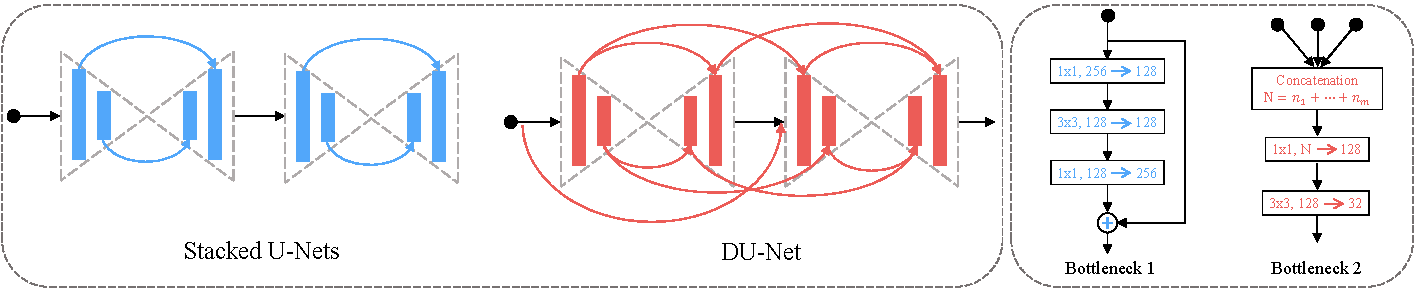
\includegraphics[width=1.0\linewidth]{figures/framework-cropped.pdf}
\caption{Illustration of stacked U-Nets and DU-Net. Stacked U-Nets has skip connections only within each U-Net. In contrast, DU-Net also connects blocks with the same semantic meanings across different U-Nets. The feature reuse could significantly reduce the size of bottleneck in each block, as shown in the right figure. Consequently, with the same number of U-Nets, DU-Net has only 30\% parameters of stacked U-Nets.}
\label{fig:framework}
\end{figure*}

% 
Our solution to those efficiency issues is threefold. {\bf First}, instead of connecting all stacked U-Nets, we only connect a U-Net to its $K$ successors. We name it as the $order$-$K$ connectivity, which aims to balance the fitting accuracy and parameter efficiency by cutting off long-distance connections. {\bf Second}, we employ a memory-efficient implementation in training. The key idea is to reuse a pre-allocated memory so all connected blocks could share the same memory. Compared with the naive implementation, this strategy makes it possible to train a very deep DU-Net (actually, $2\times$ deeper). {\bf Third}, to further improve the efficiency, we investigate an iterative design that may reduce the model size to one half. More specifically, the output of the first pass of the DU-Net is used as the input of the second pass, where detection or regression loss is applied as supervision. 

% %G%
% In view of deploying our approach on mobile devices, we further attempt to quantize weights, inputs, and gradients of DU-Net to low bit-width discrete values. This not only decreases the high precision operations but also shrinks the memory usage during training. By network quantization, the size of trained model can also be largely compressed.
% %G%
Besides shrinking the number of network parameters, we also study to further quantize each parameter. This motivates from the ubiquitous mobile applications. Although current mobile devices could carry models of dozens of MBs, deploying such networks requires high-end GPUs. However, quantized models could be accelerated by some specifically designed low-cost hardwares. Beyond only deploying models on mobile devices \cite{li2017deeprebirth}, training deep neural networks on distributed mobile devices emerges recently \cite{mcmahan2016communication}. To this end, we also try to quantize not only the model parameters but also its inputs (intermediate features) and gradients in training. This is the first attempt to investigate training landmark localizers using quantized inputs and gradients.


In summary, our key contributions are:
\begin{itemize}
    \item To the best of our knowledge, we are the first to propose quantized densely connected U-Nets for visual landmark localization, which largely improves the information flow and feature reuse at the semantic level.
    \item We propose the $order$-$K$ connectivity to balance accuracy and efficiency. It decreases the growth of model size from quadratic to linear by removing trivial connections. Experiments show it could reduce $\sim$70\% parameters of state-of-the-art landmark localizers.
    \item Very deep U-Nets can be trained using a memory-efficient implementation, where pre-allocated memory is reused by all connected blocks.
    \item We further investigate an iterative refinement that may cut down half of the model size, by forwarding DU-Net twice using either detection or regression supervision.
    %G%
    \item Different from previous efforts of quantizing only the model parameters, we are the first to quantize their inputs and gradients for better training efficiency on landmark localization tasks. By choosing appropriate quantization bit-widths for weights, inputs and gradients, quantized DU-Net achieves $\sim$75\% training memory saving with comparable performance. 
    %G%
    \item Exhaustive experiments are performed to validate DU-Net in different aspects. In both human pose estimation and face alignment, DU-Net demonstrates comparable localization accuracy and use $\sim$2\% model size compared with state-of-the-art methods.
\end{itemize}

% We are the first to deploy network quantization for better training efficiency on localization tasks. By choosing appropriate quantization bit-widths for weights, inputs and gradients, quantized DU-Net achieves at least 32$\times$ memory saving with comparable performance to the-state-of-art approaches. 


%The landmark localization such as human pose estimation \cite{toshev2014deeppose,newell2016stacked,wei2016convolutional}, facial landmark localization \cite{xiong2013supervised,zhang2014facial,sagonas2013300}, etc, plays an important role in the higher-level image understanding. The Convolutional Neural Networks (CNNs) have dominated this field, among which recent architecture of stacked hourglasses \cite{newell2016stacked}, a variant of the U-Net \cite{ronneberger2015unet}, becomes a standard solution. The skip connections between top-down and bottom-up blocks within a U-Net could preserve the spatial information and increase the gradient flow. With multiple U-Nets stacked together, the prediction could be refined stage by stage. However, the connections are only within each U-Net of the stacked hourglasses and no explicit connections exist between U-Nets, which may impede the information flow across them. And the blocks with the same semantics in different U-Nets cannot share features, leading to many redundant parameters. 

% Its success attributes to three key factors: repeated top-down, bottom-up inferences, intermediate supervisions and residual bottlenecks \cite{}. 

% The multiple stage top-down and bottom-up processing could better integrate both the local and global visual contexts into the final prediction. The intermediate supervision and residual bottlenecks, on the other hand, could alleviate the gradient vanish problem in deep networks.
%In this paper, we propose to densely connect stacked U-Nets by linking blocks with the same semantics in different U-Nets. We refer to this architecture as {\it Dense U-Nets}. The blocks in a U-Net could get direct inputs from its connected blocks in all preceding U-Nets, making the information flow more efficiently among the U-Nets. The feature reuse at each resolution could reduce the parameters in each block. The dense connectivity in our Dense U-Nets is different from that of DenseNet \cite{huang2016densely}. More specifically, layers only within each single block of the DenseNet are connected. In contrast, we connect blocks lying across the whole Dense U-Nets and connections of hierarchical blocks are mixed together. An illustration is given in Figure \ref{fig:framework}. We name it as the {\it global dense connectivity} to differentiate from the local one in the DenseNet.

% Besides, features in the Dense U-Nets are fused by the concatenation which could facilitate the information flow compared with the summation operation in the stacked hourglasses.

% Although the dense connectivity in our Dense U-Nets is similar with that of DenseNet \cite{}, 
% More recently, the DenseNet \cite{} achieves superior image classification performance over the ResNet \cite{} in terms of both the accuracy and model size, which benefits from the dense connections between layers. Its key insight is the feature reuse between layers of the same resolutions. The dense connectivity in the DenseNet, existing within one block, is local. By extending this principle, we propose a global dense connectivity, in contrast to the local connectivity in \cite{}, that blocks at the same locations of different U-Nets are connected. Hence, we refer to this architecture as {\it Dense U-Nets}. To our best knowledge, we are the first to generalize the local dense connectivity into the stacked U-Nets. 
% The global dense connectivity could make it easier to train much deeper stacked U-Nets.

% This motivates us to replace the residual modules  in the stacked hourglasses with the dense connected layers. However, this dense connectivity exists only locally within a contiguous  block in which all feature maps have the same spatial resolution. A U-Net, on the other hand, consists of a sequence of top-down and bottom-up blocks. A straight way is to turn each block into a dense block with multiple layers. However, this would sacrifice the spirit of stacked hourglasses that multiple stacked hourglasses outperform a single hourglass with multiple layers in each block.

% In order to integrate the structure of stacked U-Nets together with the idea of dense connectivity, we propose a global dense connectivity, in contrast to the local connectivity in \cite{}, that blocks at the same locations of different U-Nets are connected. Hence, we refer to this architecture as {\it Dense U-Nets}. The connected layers in the Dense U-Nets distribute along the whole network rather than in local continuous blocks. Compared with the local residual modules in the stacked hourglasses, the global dense connections could significantly facilitate the gradient to flow across stacked U-Nets.

%In practice, the Dense U-Nets have the efficiency problems of both parameter and training memory. First, suppose a Dense U-Nets contains $n$ U-Nets, there would be $O(n(n-1)/2)$ connections. Even though we use the dense bottleneck in Figure \ref{fig:framework}, the number of conv($1\times 1$) parameters still has the quadratic growth. Inspired from the Variable Order Markov (VOM) models \cite{begleiter2004prediction}, we propose the order-K connectivity that, instead of linking all the U-Nets, we connect only a fixed number of U-Nets. The goal is to use the minimum connections achieving the most obvious improvements. The multiple intermediate supervisions in the Dense U-Nets are good compensates for the order-K connectivity since they could provide additional gradients. The DenseNet does not have this advantage since it has only one supervision at the end.

% Furthermore, different from the DenseNet with only one supervision, the Dense U-Nets have multiple intermediate supervisions. The global dense connections plus the intermediate supervisions could bring faster convergence on the training set, but also gives rise to the concern of overfitting. Inspired from the Variable Order Markov (VOM) models \cite{}, we propose the order-K connectivity that, instead of linking all the U-Nets, we connect only a fixed number of U-Nets. The goal is to use the minimum connections achieving the most obvious improvement. Another advantage of order-K connectivity is that it has fewer parameters compared with the dense connectivity.

%Benefiting from the order-K connectivity, the Dense U-Nets could achieve comparable performance of stacked hourglasses with only one-third parameters. However, a naive implementation of the order-K connectivity could make the training very memory expensive. Therefore, we employ the memory efficient implementation \cite{pleiss2017memory}. The key idea is to share memories for time efficient operations such as concatenation and batch norm \cite{ioffe2015batch} within the connected layers. By pre-allocating a fixed memory, the later features produced by these operations would replace earlier features. So we need to re-compute those replaced features in the backward phase. The memory efficient implementation makes it possible to train Dense U-Nets two times deeper than the stacked hourglasses. 

%Furthermore, we also investigate to use the iterative refinement improving the parameter efficiency. Given a Dense U-Nets, we compare its performance with another Dense U-Nets with only half depth but an additional iteration. Besides, both detection and regression losses \cite{bulat2016human} were used in the landmark detection tasks, but there is no investigation yet about how they independently and collaboratively affect the prediction. We will give their detailed comparison in our experiments.

%In summary, the key contributions are:
%\begin{itemize}
%    \item To our best knowledge, we are the first to use the dense connectivity among the stacked U-Nets. The global dense connectivity in our Dense U-Nets is different from the local one in the DenseNet \cite{huang2016densely}.
%    \item We propose the order-K connectivity to make the Dense U-Nets parameter efficient. The order-K connectivity could decrease the growth of conv($1\times 1$) parameters from quadratic to linear. With comparable performance as the stacked hourglasses \cite{newell2016stacked}, it makes the Dense U-Nets require only one-third parameters. 
%    \item The memory efficient implementation of Dense U-Nets is provided to reduce its training memory usage. It makes it possible to train Dense U-Nets two times deeper than the stacked hourglasses.
%    \item We further explore using iterative refinement to improvement the parameter efficiency. At the same time, we investigate how different combinations of the detection and regression losses affect the performance.
%\end{itemize}
The majority of existing approaches to WSD formulate this task as  MIL. In this formulation an image is interpreted as a bag of regions. If the image is labeled as positive, then one of the regions is assume to tightly contain the object of interest. If the image is labeled as negative, then no region contains the object. Learning alternates between estimating a model of the object appearance and selecting which regions in the positive bags correspond to the object using the appearance model. 

The MIL strategy results in a non-convex optimization problem; in practice, solvers tend to get stuck in local optima such that the quality of the solution strongly depends on the initialization. Several papers have focused on developing various initialization strategies \cite{Kumar10a,Deselaers10,Song14a,Cinbis15} and on regularizing the optimization problem \cite{Song14,Bilen14}. Kumar~\etal \cite{Kumar10a} propose a self-paced learning strategy that progressively includes harder samples to a small set of initial ones at training. Deselaers~\etal~\cite{Deselaers10} initialize object locations based on the objectness score. Cinbis~\etal \cite{Cinbis15} propose a multi-fold split of the training data to escape local optima. Song~\etal~\cite{Song14} apply Nesterov's smoothing technique \cite{Nesterov05} to the latent SVM formulation \cite{Felzenszwalb10a} to be more robust against poor initializations. Bilen~\etal~\cite{Bilen14} propose a smoothed version of MIL that softly labels object instances instead of choosing the highest scoring ones. Additionally, their method regularizes the latent object locations by penalizing unlikely configurations based on symmetry and mutual exclusion principles.

Another line of research in WSD \cite{Song14,Song14a,Wang14a} is based on the idea of identifying the similarity between image parts. Song~\etal \cite{Song14} propose a discriminative graph-based algorithm that selects a subset of windows such that each window is connected to its nearest neighbors in positive images. In~\cite{Song14a}, the same authors extend this method to discover multiple co-occurring part configurations. Wang~\etal~\cite{Wang14a} propose an iterative technique that applies a latent semantic clustering via latent Semantic Analysis (pLSA) on the windows of positive samples and selects the most discriminative cluster for each class based on its classification performance. Bilen~\etal \cite{Bilen15} propose a formulation that jointly learns a discriminative model and enforces the similarity of the selected object regions via a discriminative convex clustering algorithm.

Recently a number of researchers \cite{Oquab14,Oquab15} have proposed weakly supervised localization principles to improve classification performance of CNNs without providing any annotation for the location of objects in images. Oquab~\etal \cite{Oquab14} employ a pre-trained CNN to compute a mid-level image representation for images of PASCAL VOC. In their follow-up work, Oquab~\etal \cite{Oquab15} modify a CNN architecture to \emph{coarsely} localize object instances in image while predicting its label. 

Jaderberg~\etal~\cite{Jaderberg15c} proposed a CNN architecture in which a subnetwork automatically pre-transforms an image in order to optimize the classification accuracy of a second subnetwork. This ``transformer network'', which is trained in an end-to-end fashion from image-level labels, is shown to align objects to a common reference frame, which is a proxy to detection. Our architecture contains a mechanism that pre-select image regions that are likely to contain the object, also trained in an end-to-end fashion; while this may seem very different, this mechanism can also be thought as learning transformations (as the ones that map the detected regions to a canonical reference frame). However, the nature of the selection process in in our and their networks are very different.

%%%%%%%%%%%%%%%%%%%%%%%%%%%%%%%%%%%%%%%%%%%%%%%%%%%%%%%%%%%
%\vspace{-10pt}
%\vspace{\sectionReduceTop}
\section{VQA Dataset Collection}
\label{sec:dataset}
%\vspace{\sectionReduceBot}
%%%%%%%%%%%%%%%%%%%%%%%%%%%%%%%%%%%%%%%%%%%%%%%%%%%%%%%%%%%
\begin{figure*}[t]
\centering
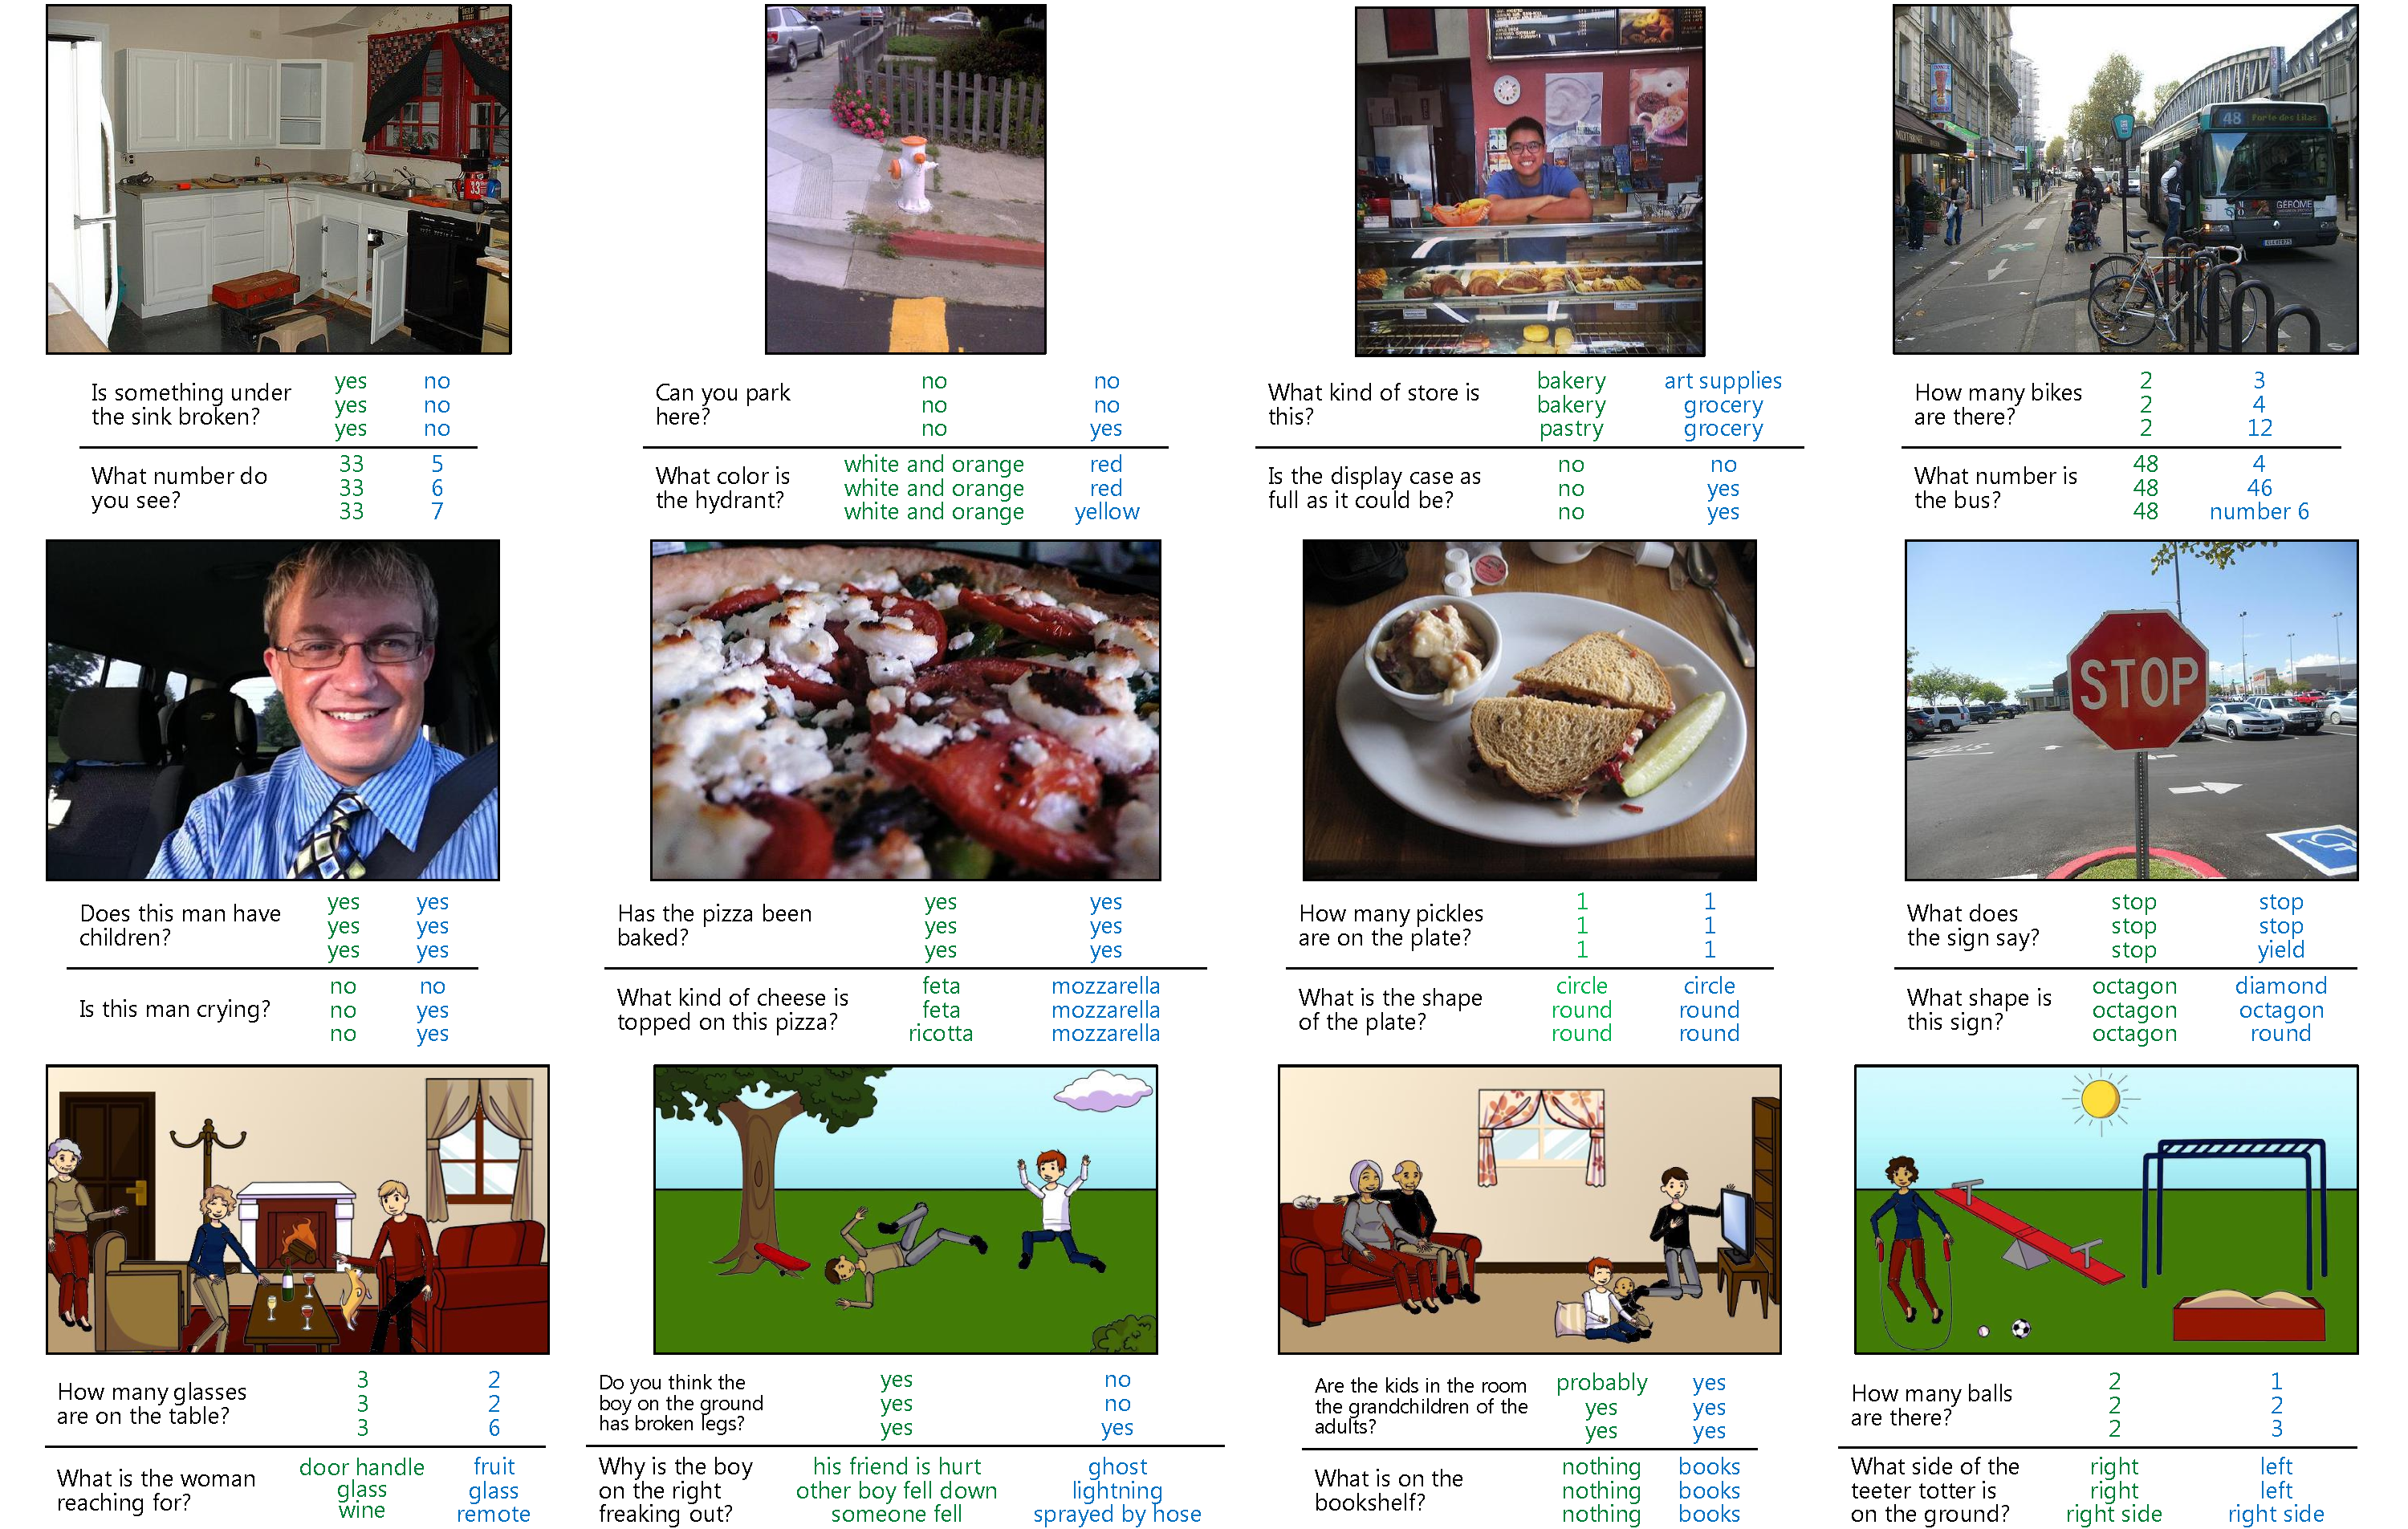
\includegraphics[width=1\linewidth]{figures/figure_02-compressed.pdf}
\caption{Examples of questions (black), (a subset of the) answers given when looking at the image (green), and answers given when not looking at the image (blue) for numerous representative examples of the dataset. See the appendix for more examples.}
%\vspace{-5pt}
\label{fig:qualResults}
%\setlength{\belowcaptionskip}{-10pt}
\end{figure*}
%%%%%%%%%%%%%%%%%%%%%%%%%%%%%%%%%%%%%%%%%%%%%%%%%%%%%%%%%%%
%%%%%%%%%%%%%%%%%%%%%%%%%%%%%%%%%%%%%%%%%%%%%%%%%%%%%%%%%%%
We now describe the Visual Question Answering (VQA) dataset. We begin by
describing the real images and abstract scenes used to collect the questions. Next, we describe
our process of collecting questions and their corresponding answers. Analysis of the questions
and answers gathered as well as baselines' \& methods' results are provided in following sections.

%\vspace{-10pt}
%\paragraph{Real Images:}
\textbf{Real Images.}
%For real images, 
We use the 123,287 training and validation images and 81,434 test images from the newly-released Microsoft
Common Objects in Context (MS COCO)~\cite{coco} dataset. The MS COCO dataset was gathered to find images containing multiple objects and rich contextual information. Given the
visual complexity of these images, they are well-suited for our VQA task. The more diverse our
collection of images, the more diverse, comprehensive, and interesting the resultant set of
questions and their answers.

%\vspace{-10pt}
%\paragraph{Abstract Scenes:}
\textbf{Abstract Scenes.}
The VQA task with real images requires the use of complex and often noisy
visual recognizers. To attract researchers interested in exploring the high-level reasoning
required for VQA, but not the low-level vision tasks, we create a new abstract scenes
dataset \cite{Antol2014,ZitnickCVPR2013,ZitnickICCV2013,VedantamPAMI2015} containing 50K scenes.
The dataset contains 20 ``paperdoll'' human models \cite{Antol2014} spanning genders, races,
and ages with 8 different expressions. The limbs are adjustable to allow
for continuous pose variations. The clipart may be used to depict both
indoor and outdoor scenes. The set contains over 100 objects and 31 animals in
various poses. The use of this clipart enables the creation of more realistic scenes (see bottom row of \figref{fig:qualResults}) that more closely mirror
real images than previous papers \cite{ZitnickCVPR2013,ZitnickICCV2013,VedantamPAMI2015}.
See the appendix
for the user interface, additional details, and examples. 

\textbf{Splits.}
For real images, we follow the same train/val/test split strategy as the MC COCO dataset~\cite{coco} 
(including test-dev, test-standard, test-challenge, test-reserve). For the VQA challenge (see section \ref{sec:challenge}), test-dev is used for debugging and validation experiments and allows for unlimited submission to the evaluation server. Test-standard is the `default' test data for the VQA competition. When comparing to the state of the art (e.g., in papers), results should be reported on test-standard. Test-standard is also used to maintain a public leaderboard that is updated upon submission. Test-reserve is used to protect against possible overfitting. If there are substantial differences between a method's scores on test-standard and test-reserve, this raises a red-flag and prompts further investigation. Results on test-reserve are not publicly revealed. Finally, test-challenge is used to determine the winners of the challenge.

For abstract scenes, we created splits for standardization, separating the scenes into 20K/10K/20K for train/val/test splits, respectively. There are no subsplits (test-dev, test-standard, test-challenge, test-reserve) for abstract scenes.
%For real images, we follow the same \texttt{train}\xspace/\texttt{val}\xspace/\texttt{test}\xspace split strategy as the MC COCO dataset~\cite{coco}. For abstract scenes, we randomly split the scenes into 20K/10K/20K train/val/test splits.}

%\vspace{-10pt}
%\paragraph{Captions.}
\textbf{Captions.}
The MS COCO dataset~\cite{coco,capeval2015} already contains five single-sentence captions for all images.
%Five captions were collected for each image.
%Upon completion, our VQA dataset will contain captions for the abstract scenes using the same user interface\footnote{\url{https://github.com/tylin/coco-ui}} for collection.
We also collected five single-captions for all abstract scenes using the same user interface\footnote{\url{https://github.com/tylin/coco-ui}} for collection.

%\vspace{-10pt}
%\paragraph{Questions:}
\textbf{Questions.}
Collecting interesting, diverse, and well-posed questions is a significant challenge.
Many simple questions may only require low-level computer vision knowledge,
such as ``What color is the cat?'' or ``How many chairs are present in the scene?''.
However, we also want questions that require commonsense knowledge about the scene,
such as ``What sound does the pictured animal make?''. Importantly, questions should also \emph{require} the image to correctly answer and not be answerable using just commonsense information, \eg, in~\figref{fig:teaser}, ``What is the mustache made of?''.  By having a wide variety of
question types and difficulty, we may be able to measure the continual progress of both
visual understanding and commonsense reasoning.

%In our pilot experiments,
We tested and evaluated a number of user interfaces for collecting
such ``interesting'' questions. % and answers.
%Numerous user interfaces were tested and evaluated.
%In order to bias towards ``meaningful'' questions,
%towards those that are more difficult,
Specifically, we ran pilot studies asking human subjects to ask questions about a given image that they believe
a ``toddler'', ``alien'', or ``smart robot'' would have trouble answering.
We found the ``smart robot'' interface to elicit the most interesting and diverse questions. 
%the ``smart robot'' questions were deemed to be
%the most interesting and diverse by the authors.
As shown in the appendix,
our final interface stated:
\begin{center}
\fbox{
\parbox{0.45\textwidth}
{``\emph{We have built a smart robot. It understands a lot about images. It can
recognize and name all the objects, it knows where the objects are, it can recognize the scene
(\eg, kitchen, beach), people's expressions and poses, and properties of objects (\eg, color of
objects, their texture). Your task is to stump this smart robot!}

\emph{Ask a question about this scene that this smart robot probably can not answer, but any human can easily answer while looking at the scene in the image.}''
}
}
\end{center}
To bias against
generic image-independent questions,
%that can be answered using generic commonsense knowledge,
subjects were instructed to ask questions that \emph{require} the image to answer. 

The same user interface was used for both the real images and abstract scenes.
In total, three questions from unique workers were gathered for each image/scene.
When writing a question, the subjects were shown the previous questions already asked for that image to
increase the question diversity. In total, the dataset contains over
$\sim$0.76M questions.


%\vspace{-10pt}
%\paragraph{Answers:}
\textbf{Answers.}
Open-ended questions result in a diverse set of possible answers.
For many questions, a simple ``yes'' or ``no'' response is sufficient. However, other questions
may require a short phrase. Multiple different answers may also be correct. For instance, the
answers ``white'', ``tan'', or ``off-white'' may all be correct answers to the same question.
Human subjects may also disagree on the ``correct'' answer, \eg, some saying ``yes'' while
others say ``no''. To handle these discrepancies, we gather \emph{10 answers for each
question from unique workers}, while also ensuring that the worker answering a question did not ask it.
We ask the subjects to provide answers that are ``a brief phrase and not a complete sentence.
Respond matter-of-factly and avoid using conversational language or inserting your opinion.''
In addition to answering the questions, the subjects were asked ``Do you think you were
able to answer the question correctly?'' and given the choices of ``no'', ``maybe'', and ``yes''. See the appendix for more details about the user interface to collect answers.
See \secref{sec:analysis} for an analysis of the answers provided.

For testing, we offer two modalities for answering the questions: (i) \textbf{open-ended} and (ii) \textbf{multiple-choice}.

For the open-ended task, the generated answers are evaluated %the percentage of
%the human subjects' answers that exactly correspond to the generated answer.
%in a round-robin fashion 
using the following accuracy metric:
%\vspace{-5pt}
\begin{equation*}
\text{accuracy} = \min(\frac{\text{\# humans that provided that answer}}{3},1)
\end{equation*}
%\vspace{-2pt}  
\ie, an answer is deemed 100\% accurate if at least 3 workers provided that exact answer.\footnote{In order 
to be consistent with `human accuracies' reported in \secref{sec:analysis}, machine accuracies are  
averaged over all ${10 \choose 9}$ sets of human annotators}
Before comparison, all responses are made lowercase, numbers converted to digits,
and punctuation \& articles removed. We avoid using soft metrics
such as Word2Vec \cite{word2vec}, since they often group together 
%similar types of 
words that we wish to distinguish, such as ``left'' and ``right''. We also avoid using evaluation metrics from machine translation such as BLEU and ROUGE because such metrics are typically applicable and reliable for sentences containing multiple words. In VQA, most answers (89.32\%) are single word; thus there no high-order n-gram matches between predicted answers and ground-truth answers, and low-order n-gram matches degenerate to exact-string matching. Moreover, these automatic metrics such as BLEU and ROUGE have been found to poorly correlate with human judgement for tasks such as image caption evaluation \cite{DBLP:journals/corr/ChenFLVGDZ15}.

For multiple-choice task, 18 candidate answers are created for each question. As with the open-ended task,
the accuracy of a chosen option is computed based on the number of human subjects who provided 
that answer (divided by 3 and clipped at 1). We generate a candidate set of correct
and incorrect answers from four sets of answers:
%\begin{compactitem}
%\begin{asparaitem}
%\item 
\textbf{Correct:} The most common (out of ten) correct answer.
%\item 
\textbf{Plausible:} To generate incorrect, but still plausible answers we ask
three subjects to answer the questions without seeing the image. See the appendix for more details about the user interface to collect these answers. If three unique answers
are not found, we gather additional answers from nearest neighbor questions
using a bag-of-words model. The use of these answers helps ensure the image,
and not just commonsense knowledge, is necessary to answer the question.
%\item 
\textbf{Popular:} These are the 10 most popular answers. For instance, these are ``yes'',
``no'', ``2'', ``1'', ``white'', ``3'', ``red'', ``blue'', ``4'', ``green'' for real images.
%and ``yes'', ``no'', ``2'', ``1'', ``red'', ``3'', ``white'', ``4'', ``blue'', ``yellow'' for abstract images.}
The inclusion of the most popular answers makes it more difficult for algorithms to infer the type of
question from the set of answers provided, \ie, learning that it is a ``yes or no'' question just because
``yes'' and ``no'' are present in the answers.
%\item 
\textbf{Random:} Correct answers from random questions in the dataset.
%Random answers from other questions. 
To generate a total of 18 candidate answers, we first find the union of the correct, plausible, and popular answers. 
We include random answers until 18 unique answers are found.
%\end{compactitem}
%\end{asparaitem}
The order of the answers is randomized. Example multiple choice questions are in the appendix.

Note that all 18 candidate answers are unique. But since 10 different subjects answered every question, it is possible that more than one of those 10 answers be present in the 18 choices. In such cases, according to the accuracy metric, multiple options could have a non-zero accuracy.
\section{VQA Dataset Analysis}
\label{sec:analysis}
%\vspace{\sectionReduceBot}
%%%%%%%%%%%%%%%%%%%%%%%%%%%%%%%%%%%%%%%%%%%%%%%%%%%%%%%%%%%
%%%%%%%%%%%%%%%%%%%%%%%%%%%%%%%%%%%%%%%%%%%%%%%%%%%%%%%%%%%
\begin{figure*}[t]
\centering
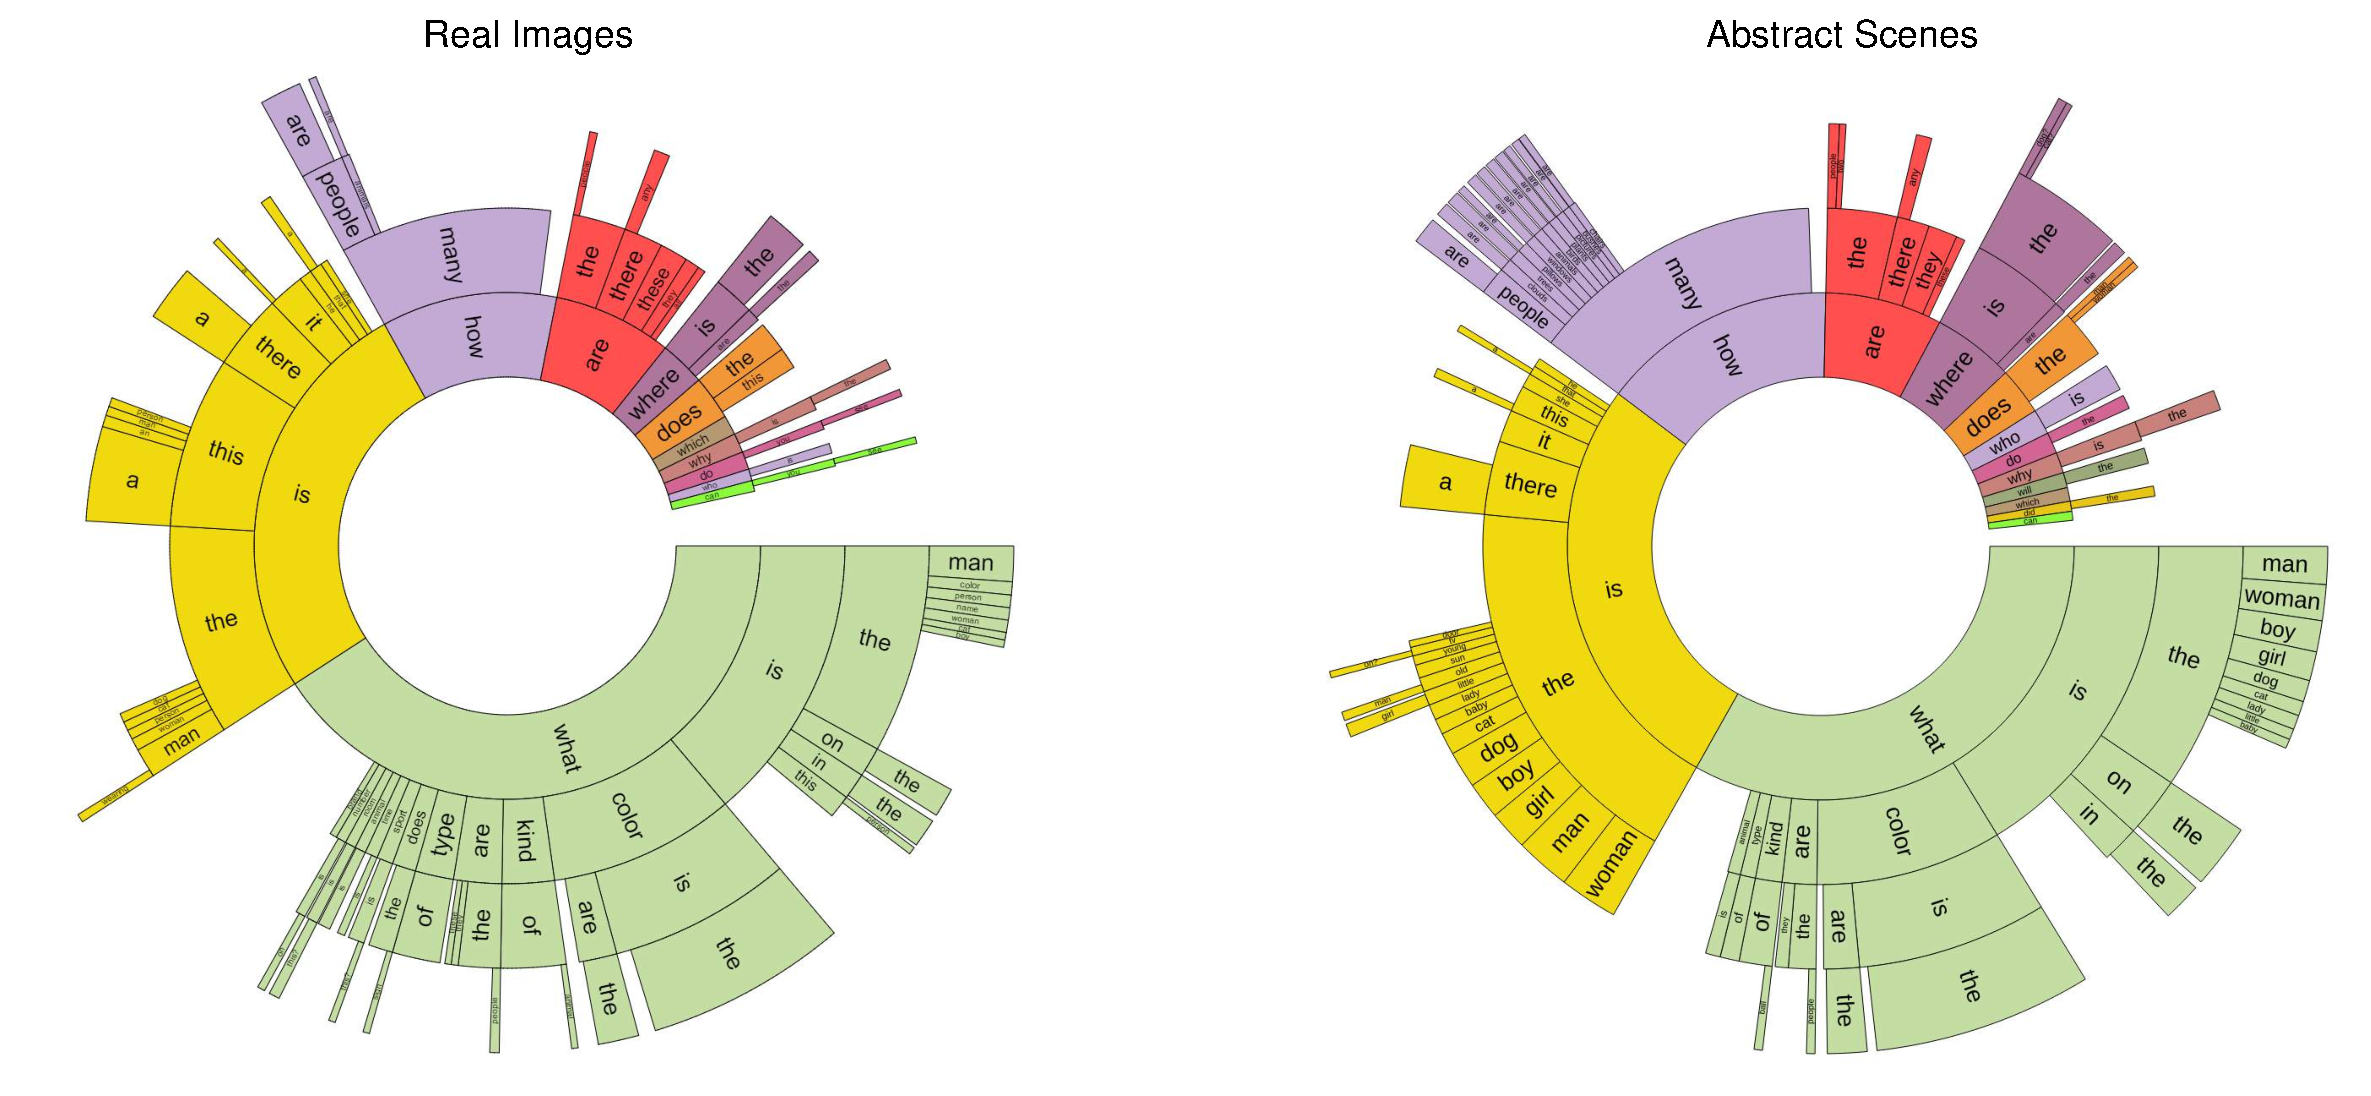
\includegraphics[width=1\linewidth]{figures/QuestionTypes3.pdf}
\caption{Distribution of questions by their first four words for a random sample of 60K questions for real images (left) and all questions for abstract scenes (right). The ordering of the words starts towards the center and radiates outwards. The arc length is proportional to the number of questions containing the word. White areas are words with contributions too small to show. }
%\vspace{-5pt}
\label{fig:QuesCluster}
%\setlength{\belowcaptionskip}{-10pt}
\end{figure*}
%%%%%%%%%%%%%%%%%%%%%%%%%%%%%%%%%%%%%%%%%%%%%%%%%%%%%%%%%%%

In this section, we provide an analysis of the questions and answers in the VQA train dataset.
To gain an understanding of the types of questions asked and answers provided, we visualize
the distribution of question types and answers. We also explore how often the questions may
be answered without the image using just commonsense information. Finally, we analyze whether
the information contained in an image caption is sufficient to answer the questions.

The dataset includes 614,163 questions 
%and a total of 
and 7,984,119 answers (including answers provided by workers with and without 
looking at the image) 
%and without looking at the image) 
for 204,721 images from the MS COCO dataset~\cite{coco} and 150,000 questions with 1,950,000 answers for $50,000$ abstract scenes.

%\textcolor{red}{
%We emphasize that the creation of a dataset of this scale and richness
%is a time consuming process, taking months to complete.
%While the entirety of the dataset has been collected,} at the time of original submission,
%120,520 questions with 270,210 answers for 50,000 MS COCO
%images and 30,000 questions with 79,740 answers for 10,000 abstract scenes had been collected.
%Please refer to the appendix for further details.
%\textcolor{red}{The results in this section still reflect that subset of the final dataset.}
%We emphasize that the creation of a dataset of this scale and richness
%is a time consuming process, taking months to complete.
%By our current estimates,
%approximately 5,000 questions and 40,000 answers are collected per day
%using Amazon Mechanical Turk (AMT).
%The entire dataset will take approximately three months to complete. At the time of submission,
%120,520 questions with 270,210 answers for 50,000 MS COCO
%images and 30,000 questions with 79,740 answers for 10,000 abstract scenes had been collected.
%Please refer to the appendix for further details.


%%%%%%%%%%%%%%%%%%%%%%%%%%%%%%%%%%%%%%%%%%%%%%%%%%%%%%%%%%%
%\vspace{\subsectionReduceTop}
\subsection{Questions}
%\vspace{\subsectionReduceBot}
%%%%%%%%%%%%%%%%%%%%%%%%%%%%%%%%%%%%%%%%%%%%%%%%%%%%%%%%%%%

\textbf{Types of Question.}
Given the structure of questions generated in the English language,
we can cluster questions into different types based on the words that start the question.
\figref{fig:QuesCluster} shows the distribution of questions based on the first four
words of the questions for both the real images (left) and abstract scenes (right).
Interestingly, the distribution of questions is quite similar for both real images and abstract scenes.
This helps demonstrate that the type of questions elicited by the abstract scenes is similar to
those elicited by the real images. There exists a surprising variety of question types,
including ``What is$\ldots$'', ``Is there$\ldots$'', ``How many$\ldots$'', and ``Does the$\ldots$''.
Quantitatively, the percentage of questions for different types is shown in \tableref{tab:typeacc}. Several example questions and answers are shown in \figref{fig:qualResults}.
%\textbf{Sub-Types.}
A particularly interesting type of question is the ``What is$\ldots$'' questions, since they have a
diverse set of possible answers. See the appendix for visualizations for ``What is$\ldots$'' questions.

\textbf{Lengths.}
\figref{fig:QuesLen} shows the distribution of question lengths.
We see that most questions range from four to ten words.


\begin{comment}\begin{table}[h]
{\small
\begin{tabular}{@{\extracolsep{\fill}}p{2cm}|ccccc@{\extracolsep{\fill}}}
%\toprule
Dataset  & Yes & No\\
%\midrule
Real   & 18.21 & 14.06 \\
Abstract & 26.54 & 16.70 \\
\end{tabular}
}
\vspace{5pt}
\caption{Percentage of ``yes'' and ``no'' questions in the real and abstract datasets.}
\label{table:yesno}
%\vspace{\captionReduceBot}
\end{table}
\end{comment}

%%%%%%%%%%%%%%%%%%%%%%%%%%%%%%%%%%%%%%%%%%%%%%%%%%%%%%%%%%%
\begin{figure}[t]
\centering
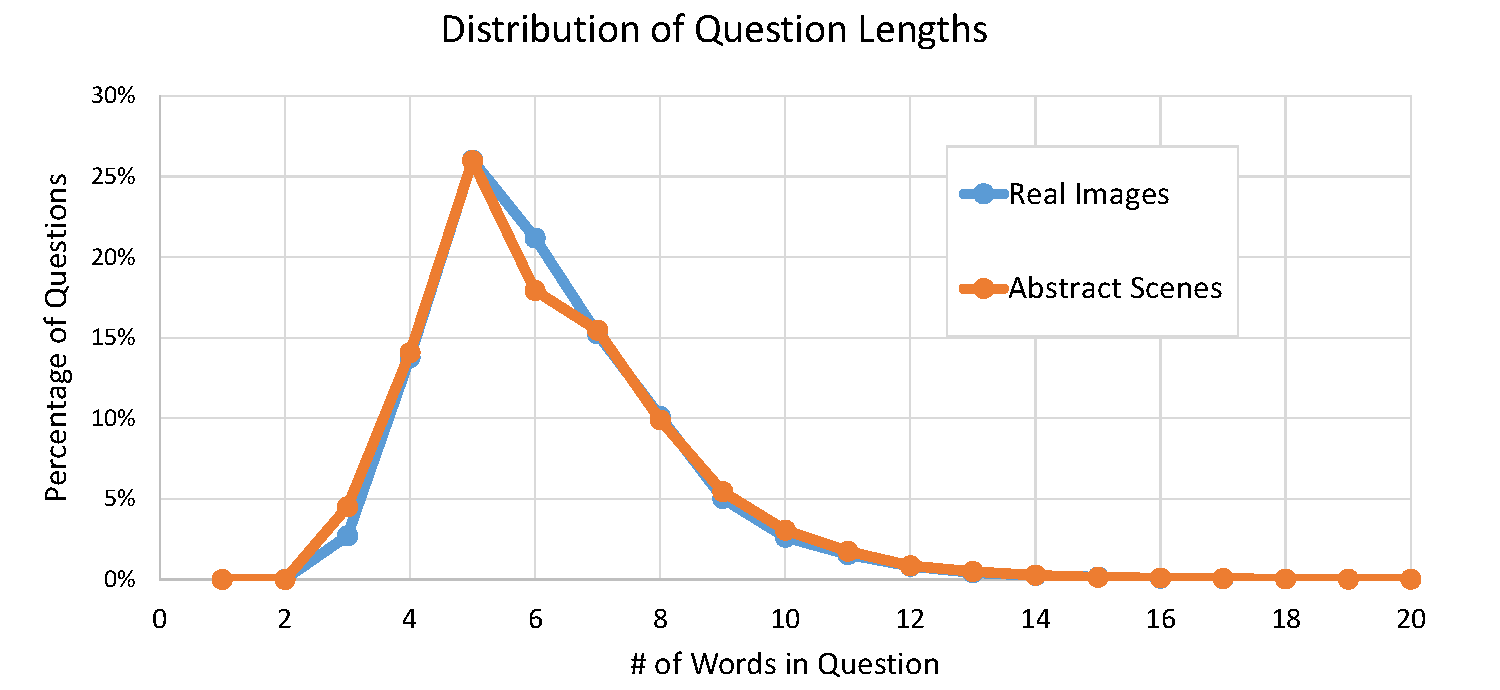
\includegraphics[width=1\linewidth]{figures/Lengths.pdf}
%\vspace{-9pt}
\caption{Percentage of questions with different word lengths for real images and abstract scenes.}
%\vspace{-5pt}
\label{fig:QuesLen}
%\setlength{\belowcaptionskip}{-10pt}
\end{figure}
%%%%%%%%%%%%%%%%%%%%%%%%%%%%%%%%%%%%%%%%%%%%%%%%%%%%%%%%%%%




\begin{figure*}
\centering
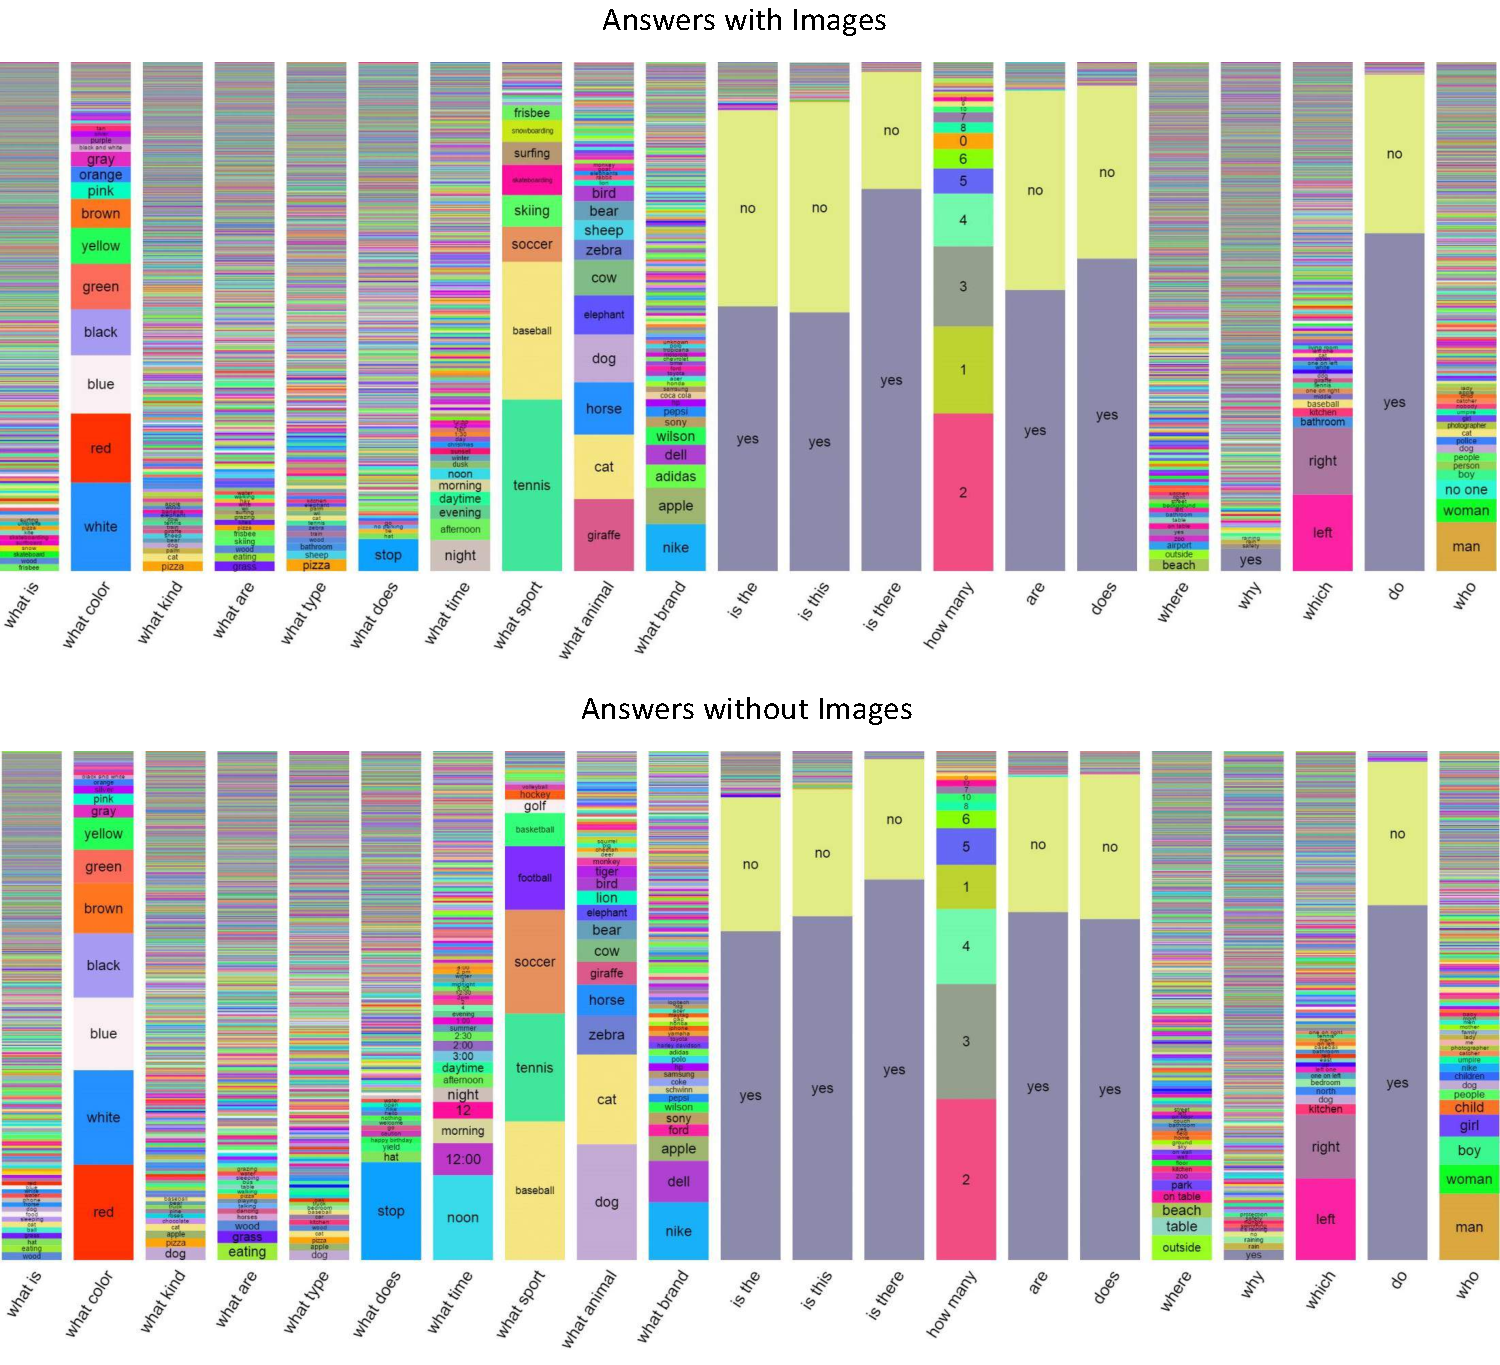
\includegraphics[width=1\linewidth]{figures/answers.pdf}
%\vspace{-5pt}
\caption{Distribution of answers per question type for a random sample of 60K questions for real images when subjects provide answers when given the image (top) and when not given the image (bottom).}
%\vspace{-5pt}
\label{fig:AnsPerQues}
%\setlength{\belowcaptionskip}{-10pt}
\end{figure*}


%%%%%%%%%%%%%%%%%%%%%%%%%%%%%%%%%%%%%%%%%%%%%%%%%%%%%%%%%%%
%\vspace{\subsectionReduceTop}
\subsection{Answers}
%\vspace{\subsectionReduceBot}
%%%%%%%%%%%%%%%%%%%%%%%%%%%%%%%%%%%%%%%%%%%%%%%%%%%%%%%%%%%

%\textbf{Typical Answers for Different Question Types.}
\textbf{Typical Answers.}
%Next, we analyze the answers provided for different question types.
\figref{fig:AnsPerQues} (top) shows the distribution of answers for several question types.
We can see that a number of question types, such as ``Is the\ldots'', ``Are\ldots'', and ``Does\ldots'' are
typically answered using ``yes'' and ``no'' as answers.
%\textcolor{red}{Question types such as ``How many\ldots'' are answered using numbers. $12.31\%$ and $14.48\%$ of the questions are answered using numbers on real images and abstract scenes, respectively.}
Other questions such as ``What is\ldots'' and ``What type\ldots'' have a rich diversity
of responses. Other question types such as ``What color\ldots'' or ``Which\ldots'' have more specialized responses,
such as colors, or ``left'' and ``right''. 
See the appendix for a list of the most popular answers.

\textbf{Lengths.}
Most answers consist of a single word, with the distribution of answers containing one, two, or three words, respectively being $89.32\%$, $6.91\%$, and $2.74\%$ for real images and $90.51\%$, $5.89\%$, and $2.49\%$ for abstract scenes.
%$89.16\%$, $7.00\%$, and $2.77\%$ of answers containing one, two, or three words, respectively.
The brevity of answers is not surprising, since the questions tend to elicit specific
information from the images. This is in contrast with image captions that generically
describe the entire image and hence tend to be longer. The brevity of our answers makes
automatic evaluation feasible. While it may be tempting to believe the brevity of the answers
makes the problem easier, recall that they are human-provided open-ended answers to
open-ended questions. The questions typically require complex reasoning to arrive at these
deceptively simple answers (see \figref{fig:qualResults}).
There are currently 23,234 unique one-word answers in our dataset for real images and 3,770 for abstract scenes.
%There are currently 10,011 unique one-word answers in our dataset.

\textbf{`Yes/No' and `Number' Answers.}
Many questions are answered using either ``yes'' or ``no'' (or sometimes ``maybe'') -- 
$38.37\%$ and $40.66\%$ of the questions on real images and abstract scenes respectively. 
Among these `yes/no' questions, there is a bias towards %answering with 
``yes'' -- %with ``yes'' being preferred %$61.32\%$ and $58.46\%$ 
$58.83\%$ and $55.86\%$ of `yes/no' answers are ``yes'' for real images and abstract scenes. 
Question types such as ``How many\ldots'' are answered using numbers -- 
$12.31\%$ and $14.48\%$ of the questions on real images and abstract scenes are `number' questions. 
``2'' is the most popular answer among the `number' questions, making up 
$26.04\%$ of the `number' answers for real images and $39.85\%$ for abstract scenes. 

\textbf{Subject Confidence.}
When the subjects answered the questions, we asked
``Do you think you were able to answer the question correctly?''.
\figref{fig:ConfScores} shows the distribution of responses. A majority of the answers
were labeled as confident for both real images and abstract scenes. % respectively.

\textbf{Inter-human Agreement.}
Does the self-judgment of confidence correspond to the answer agreement between subjects?
\figref{fig:ConfScores} shows the percentage of questions in which 
(i) $7$ or more, 
(ii) $3-7$, or 
(iii) less than $3$ subjects agree on the answers given their average confidence score 
(0 = not confident, 1 = confident).
As expected, the agreement between subjects increases with confidence.
However, even if all of the subjects are confident the answers may still vary.
This is not surprising since some answers may vary, yet have very similar meaning, such as ``happy'' and ``joyful''.

\begin{figure}[t]
\centering
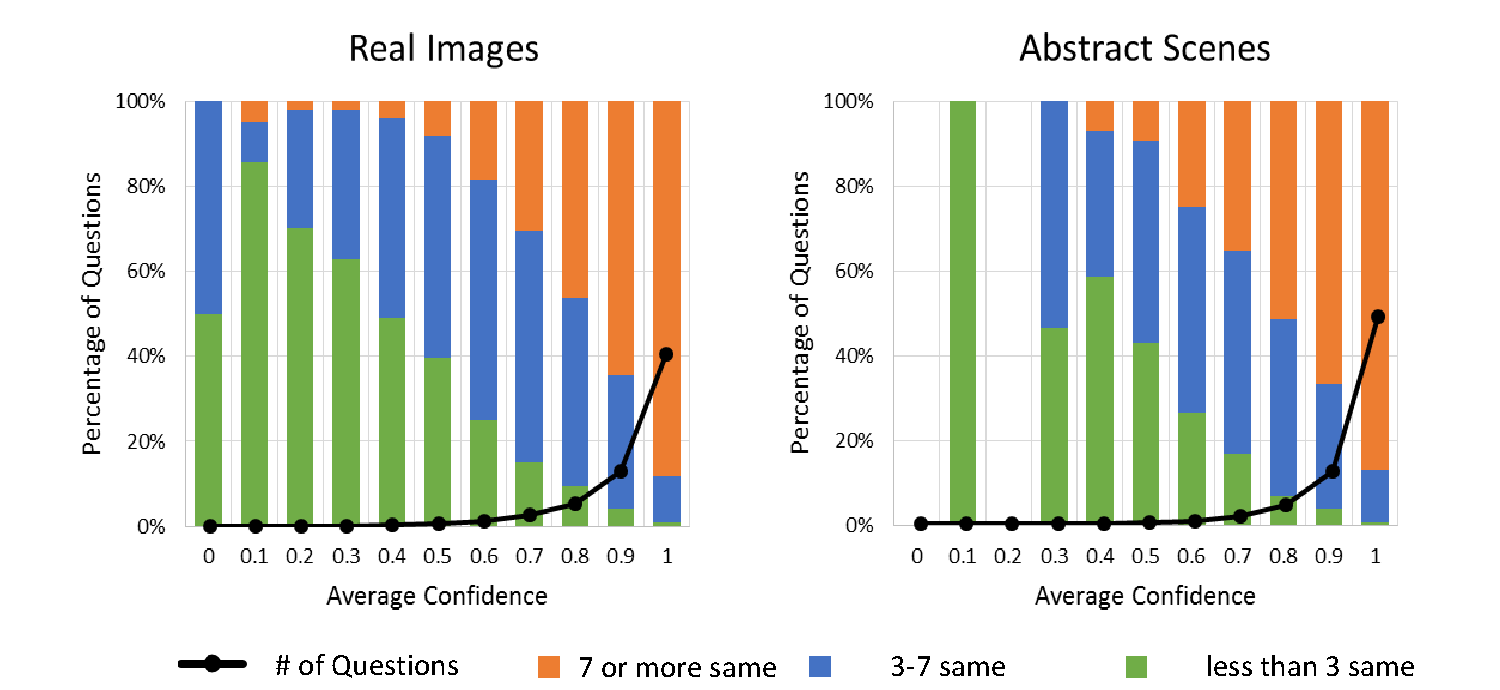
\includegraphics[width=1\linewidth]{figures/Confidence.pdf}
%\vspace{-5pt}
\caption{Number of questions per average confidence score (0 = not confident, 1 = confident) for real images and abstract scenes (black lines). Percentage of questions where 7 or more answers are same, 3-7 are same, less than 3 are same (color bars). }
%\vspace{-7pt}
\label{fig:ConfScores}
%\setlength{\belowcaptionskip}{-10pt}
\end{figure}

As shown in \tableref{table:commonsense_acc} (Question + Image), there is significant inter-human
agreement in the answers for both real images ($83.30\%$) and abstract scenes ($87.49\%$). 
%when humans are provided both the question and image while answering the question.
Note that on average each question has $2.70$ unique answers for real images and $2.39$ for abstract scenes. 
The agreement is significantly higher ($>95\%$) for \quotes{yes/no} questions and lower for other questions ($<76\%$), possibly due to the fact that we perform exact string matching and do not account for synonyms, plurality, \etc. Note that the automatic determination of synonyms is a difficult problem, since the level of answer granularity can vary across questions.




%%%%%%%%%%%%%%%%%%%%%%%%%%%%%%%%%%%%%%%%%%%%%%%%%%%%%%%%%%%
%\vspace{\subsectionReduceTop}
\subsection{Commonsense Knowledge}
\label{sec:cs}
%\vspace{\subsectionReduceBot}
%%%%%%%%%%%%%%%%%%%%%%%%%%%%%%%%%%%%%%%%%%%%%%%%%%%%%%%%%%%
\begin{figure*}[t]
 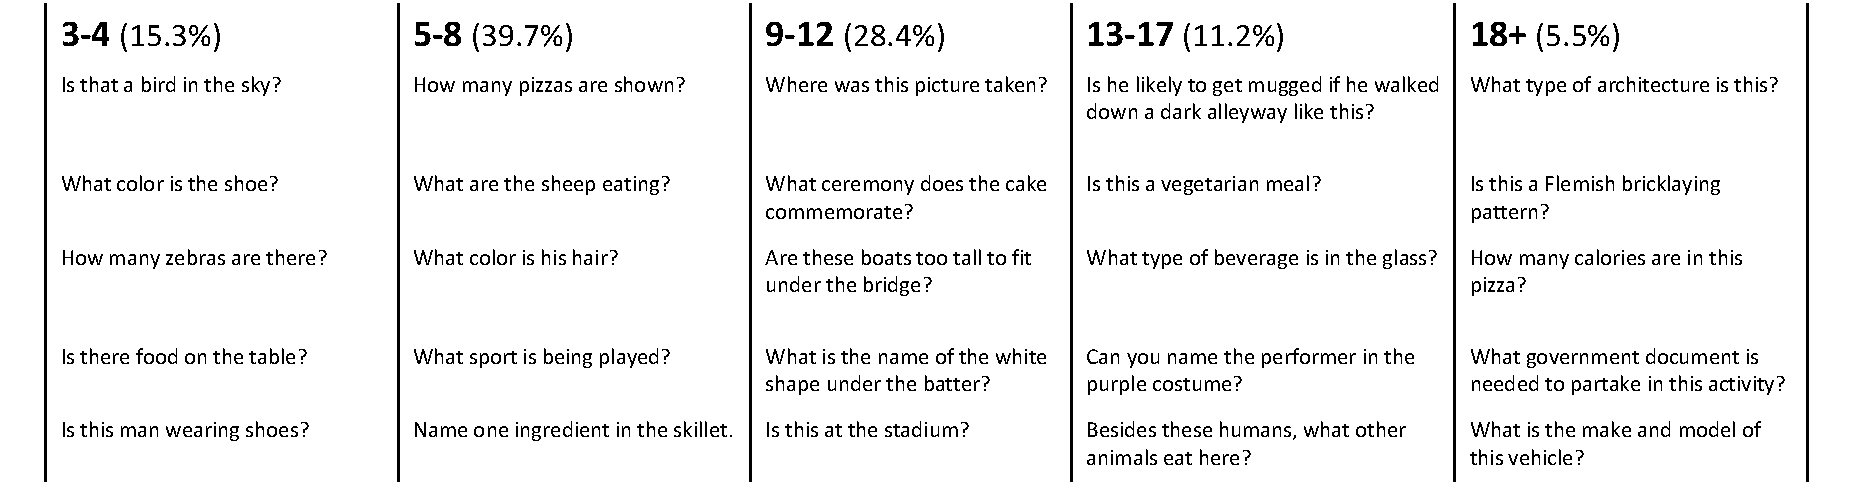
\includegraphics[width=\linewidth]{figures/age.pdf}
 \centering
\caption{\small Example questions judged by Mturk workers to be answerable by different age groups. The percentage of questions falling into each age group is shown in parentheses.}
 \label{fig:age}
 \end{figure*}
 	
\textbf{Is the Image Necessary?}
%Can the questions be answered using commonsense knowledge alone without the need for an image,
%\eg, ``What is the color of the sheep?''?
Clearly, some questions can sometimes be
answered correctly using commonsense knowledge alone without the need for an image,
\eg, ``What is the color of the fire hydrant?''.
We explore this issue by asking three subjects to answer
the questions \emph{without seeing the image} (see the examples in blue in \figref{fig:qualResults}).
In \tableref{table:commonsense_acc} (Question), we show the percentage of questions for which
the correct answer is provided over all questions, ``yes/no'' questions, and the other questions that
are not ``yes/no''. For ``yes/no'' questions, the human subjects respond better than chance.
For other questions, humans are only correct about $21\%$ of the time. This demonstrates that
understanding the visual information is critical to VQA and that commonsense information alone is not sufficient.

To show the qualitative difference in answers provided with and without images,
we show the distribution of answers for various question types in \figref{fig:AnsPerQues} (bottom).
The distribution of colors, numbers, and even ``yes/no'' responses is surprisingly different for answers
with and without images.
 
\textbf{Which Questions Require Common Sense?}
In order to identify questions that require commonsense reasoning to answer, we conducted 
two AMT studies (on a subset 10K questions from the real images of VQA trainval) asking subjects --
\begin{compactenum} 
\item Whether or not they believed a question required commonsense to answer the question, and 
\item The youngest age group that they believe a person must be in order to be able to correctly answer the question -- 
toddler (3-4), 
younger child (5-8), 
older child (9-12), 
teenager (13-17), 
adult (18+).
\end{compactenum}
Each question was shown to 10 subjects. We found that 
for $47.43\%$ of questions 3 or more subjects voted `yes' to commonsense, 
($18.14\%$: 6 or more).  
In the `perceived human age required to answer question' study, we found the following distribution of responses: 
toddler: $15.3\%$,
younger child: $39.7\%$, 
older child: $28.4\%$, 
teenager: $11.2\%$, 
adult: $5.5\%$.
In Figure \ref{fig:age} we show several questions for which a majority of subjects picked the specified age range. Surprisingly the perceived age needed to answer the questions is fairly well distributed across the different age ranges. As expected the questions that were judged answerable by an adult (18+) generally need specialized knowledge, whereas those answerable by a toddler (3-4) are more generic.
 
We measure the degree of commonsense required to answer a question as the percentage of subjects (out of 10) who voted ``yes'' in our ``whether or not a question requires commonsense'' study.
A fine-grained breakdown of average age and average degree of common sense (on a scale of $0-100$) required to answer a question is shown in \tableref{tab:typeacc}. The average age and the average degree of commonsense across all questions is $8.92$ and $31.01\%$ respectively. 

%\arxiv{To compute average age and average degree of commonsense across questions, we first compute the average age and average degree of commonsense (binary response scaled to $0-100$) per question (by taking average across 10 subjects for each question) and then take average across questions.} 

It is important to distinguish between:
\begin{compactenum}
\item How old someone needs to be to be able to answer a question correctly,  and
\item How old people \emph{think} someone needs to be to be able to answer a question correctly. 
\end{compactenum}

Our age annotations capture the latter -- perceptions of MTurk workers in an uncontrolled environment. As such, the relative ordering of question types in \tableref{tab:typeacc} is more important than absolute age numbers.
%The relative ordering of question types is more important than the absolute age numbers. It is important to note that the age annotations we have collected are just perceived ages: how old people -- untrained MTurk workers in an uncontrolled environment -- \emph{think} someone needs to be to be able to answer a question correctly.}
The two rankings of questions in terms of common sense required according to the two studies 
were largely correlated (Pearson's rank correlation: 0.58). 

%%%%%%%%%%%%%%%%%%%%%%%%%%%%%%%%%%%%%%%%%%%%%%%%%%%%%%%%%%%
\begin{table}[t]
\setlength{\tabcolsep}{3.2pt}
{\small
\begin{center}
%\begin{tabular}{@{}llccc@{}}
%\toprule
%Dataset & Input & All & Yes/No & Other \\
%%\hline
%\midrule
%    & Question & 40.81 & 67.60 & 21.22 \\
%Real   & Question + Caption* & 57.47 & 78.97 & 44.41 \\
%    & Question + Image & 83.30 & 95.77 & 72.67 \\
%%\hline
%\midrule
% & Question & 43.27 & 66.65 &  23.66 \\
%Abstract & Question + Caption* & 54.34 & 74.70 & 40.18 \\
% & Question + Image & 87.49 & 95.96 & 75.33 \\
%\bottomrule
%\end{tabular}
\begin{tabular}{@{}llcccc@{}}
\toprule
Dataset & Input & All & Yes/No & Number & Other \\
%\hline
\midrule
    & Question & 40.81 & 67.60 & 25.77 & 21.22 \\
Real   & Question + Caption* & 57.47 & 78.97 & 39.68 & 44.41 \\
    & Question + Image & 83.30 & 95.77 & 83.39 & 72.67 \\
%\hline
\midrule
 & Question & 43.27 & 66.65 & 28.52 & 23.66 \\
Abstract & Question + Caption* & 54.34 & 74.70 & 41.19 & 40.18 \\
 & Question + Image & 87.49 & 95.96 & 95.04 & 75.33 \\
\bottomrule
\end{tabular}
\end{center}
}
%\vspace{-7pt}
\caption {Test-standard accuracy of human subjects when asked to answer the 
question without seeing the image (Question), 
seeing just a caption of the image and not the image itself (Question + Caption), 
and seeing the image (Question + Image). 
Results are shown for all questions, ``yes/no'' \& ``number'' questions, and other questions 
that are neither answered ``yes/no'' nor number. 
All answers are free-form and not multiple-choice. 
*\hspace{1pt}These accuracies are evaluated on a subset of 3K train questions (1K images).}
% \textcolor{red}{and are not directly comparable to the corresponding numbers in older version.}}
\label{table:commonsense_acc}
%\vspace{\captionReduceBot}
%\vspace{-5pt}
\end{table}
%%%%%%%%%%%%%%%%%%%%%%%%%%%%%%%%%%%%%%%%%%%%%%%%%%%%%%%%%%%


%%%%%%%%%%%%%%%%%%%%%%%%%%%%%%%%%%%%%%%%%%%%%%%%%%%%%%%%%%%
%\vspace{\subsectionReduceTop}
\subsection{Captions \textbf{\vs} Questions}
%\vspace{\subsectionReduceBot}
%%%%%%%%%%%%%%%%%%%%%%%%%%%%%%%%%%%%%%%%%%%%%%%%%%%%%%%%%%%


Do generic image captions provide enough information to answer the questions?
\tableref{table:commonsense_acc} (Question + Caption) shows the percentage of questions answered
correctly when human subjects are given the question and a human-provided caption
describing the image, but not the image. As expected, the results are better than when humans are shown the questions alone.
However, the accuracies are significantly lower than when subjects are shown the actual image.
This demonstrates that in order to answer the questions correctly, deeper image understanding 
(beyond what image captions typically capture) is necessary. In fact, we find that the distributions of nouns, verbs, and adjectives mentioned in captions is statistically significantly different from those mentioned in our questions + answers (Kolmogorov-Smirnov test, $p<.001$) for both real images and abstract scenes. See the appendix for details. 
%This motivates the VQA task as a way to learn further information about visual scenes.
%\vspace{\sectionReduceTop}
\section{VQA Baselines and Methods}
%\vspace{\sectionReduceBot}
\begin{figure*}[h]
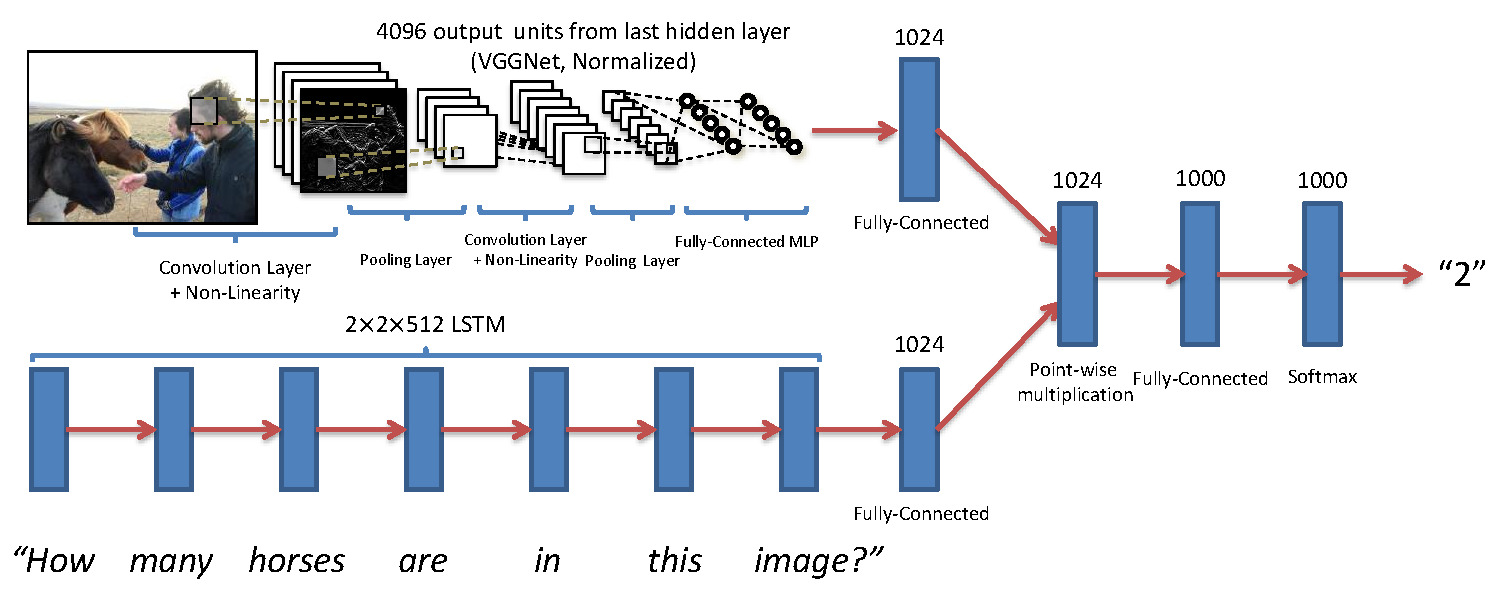
\includegraphics[width=1\linewidth]{figures/best_model_compressed.pdf}
\centering
\caption{Our best performing model (deeper LSTM Q + norm I). This model uses a two layer LSTM to encode the questions and the last hidden layer of VGGNet~\cite{Simonyan14c} to encode the images. The image features are then $\ell_2$ normalized. Both the question and image features are transformed to a common space and fused via element-wise multiplication, which is then passed through a fully connected layer followed by a softmax layer to obtain a distribution over answers.}
\label{fig:best_model}
%\vspace{\captionReduceBot}
\end{figure*}
In this section, we explore the difficulty of the VQA dataset for the MS COCO images using several baselines 
and novel methods. We train on VQA train+val. Unless stated otherwise, all human accuracies are on test-standard, machine accuracies are on test-dev, and results involving human captions (in gray font) are trained on train and tested on val (because captions are not available for test). 

\subsection{Baselines}
\label{sec:baselinesmain}
We implemented the following baselines:
\begin{enumerate}
\item \textbf{random:} We randomly choose an answer from the top 1K answers of the VQA train/val dataset.

\item \textbf{prior (``yes''):} We always select the most popular answer (``yes'') for both the open-ended and multiple-choice tasks. Note that ``yes'' is always one of the choices for the multiple-choice questions.

\item \textbf{per Q-type prior:} For the open-ended task, we pick the most popular answer per question type (see the appendix for details). For the multiple-choice task, we pick the answer (from the provided choices) that is most similar to the picked answer for the open-ended task using cosine similarity in Word2Vec\cite{word2vec} feature space.

\item \textbf{nearest neighbor:} Given a test image, question pair, we first find the $K$ nearest neighbor questions and associated images from the training set. See appendix for details on how neighbors are found. Next, for the open-ended task, we pick the most frequent ground truth answer from this set of nearest neighbor question, image pairs. Similar to the ``per Q-type prior'' baseline, for the multiple-choice task, we pick the answer (from the provided choices) that is most similar to the picked answer for the open-ended task using cosine similarity in \\ Word2Vec\cite{word2vec} feature space.
\end{enumerate}

%If we randomly choose an answer from the top 1K answers of the VQA train/val dataset, 
%the test-standard accuracy is $0.12\%$. 
%If we always select the most popular answer (``yes''), the accuracy is $29.72\%$. Picking the most popular answer per question type does $37.55\%$ and a nearest neighbor approach does $42.73\%$ on test-standard (see the appendix for details).
%For testing, we use the same train/val/test splits as COCO$^2$. 
%we split our real image dataset into a training and testing dataset. Our training dataset contains $30,000$ images and our testing dataset contains $20,000$ images. \jiasen{change image numbers, also including the NN baseline?}
\vspace{-5pt}
\subsection{Methods}
\label{sec:methods}
For our methods, we develop a 2-channel vision (image) + language (question) model that culminates with a softmax over $K$ possible outputs. We choose the top $K = 1000$ most frequent answers as possible outputs. This set of answers covers $82.67\%$ of the train+val answers. We describe the different components of our model below:

\textbf{Image Channel:} This channel provides an embedding for the image. We experiment with two embeddings -- 
\begin{compactenum}
\item \textbf{I:} The activations from the last hidden layer of VGGNet~\cite{Simonyan14c} are used as 4096-dim image embedding.
\item \textbf{norm I:} These are $\ell_2$ normalized activations from the last hidden layer of VGGNet~\cite{Simonyan14c}.
\end{compactenum}

\textbf{Question Channel:} This channel provides an embedding for the question. We experiment with three embeddings --
\begin{compactenum}
\item \textbf{Bag-of-Words Question (BoW Q)}: The top 1,000 words in the questions are used to create a bag-of-words representation. Since there is a strong correlation between the words that start a question and the answer (see \figref{fig:AnsPerQues}), we find the top 10 first, second, and third words of the questions and create a 30 dimensional bag-of-words representation. These features are concatenated to get a 1,030-dim embedding for the question.
\item \textbf{LSTM Q:} An LSTM with one hidden layer is used to obtain 1024-dim embedding for the question. The embedding obtained from the LSTM is a concatenation of last cell state and last hidden state representations (each being 512-dim) from the hidden layer of the LSTM. Each question word is encoded with 300-dim embedding by a fully-connected layer + tanh non-linearity which is then fed to the LSTM. The input vocabulary to the embedding layer consists of all the question words seen in the training dataset.
\item \textbf{deeper LSTM Q:} An LSTM with two hidden layers is used to obtain 2048-dim embedding for the question. The embedding obtained from the LSTM is a concatenation of last cell state and last hidden state representations (each being 512-dim) from each of the two hidden layers of the LSTM. Hence 2 (hidden layers) x 2 (cell state and hidden state) x 512 (dimensionality of each of the cell states, as well as hidden states) in \figref{fig:best_model}. This is followed by a fully-connected layer + tanh non-linearity to transform 2048-dim embedding to 1024-dim. The question words are encoded in the same way as in LSTM Q.   
\end{compactenum}

\textbf{Multi-Layer Perceptron (MLP):} The image and question embeddings 
%obtained from the image and question channels respectively 
are combined to obtain a single embedding. 
\begin{compactenum}
\item For \textbf{BoW Q + I} method, we simply concatenate the BoW Q and I embeddings. 
\item For \textbf{LSTM Q + I}, and \textbf{deeper LSTM Q + norm I} (\figref{fig:best_model}) methods, the image embedding is first transformed to 1024-dim by a fully-connected layer + tanh non-linearity to match the LSTM embedding of the question. The transformed image and LSTM embeddings (being in a common space) are then fused via element-wise multiplication. 
\end{compactenum}
This combined image + question embedding is then passed to an MLP -- a fully connected neural network classifier with 2 hidden layers and 1000 hidden units (dropout 0.5) in each layer with tanh non-linearity, followed by a softmax layer to obtain a distribution over $K$ answers. The entire model is learned end-to-end with a cross-entropy loss. VGGNet parameters are frozen to those learned for ImageNet classification and not fine-tuned in the image channel.   

We also experimented with providing captions as input to our model. Similar to \tableref{table:commonsense_acc}, we assume that a human-generated caption is given as input. We use a bag-of-words representation containing the 1,000 most popular words in the captions as the caption embedding (\textbf{Caption}). For \textbf{BoW Question + Caption (BoW Q + C)} method, we simply concatenate the BoW Q and C embeddings. 
%\jiasen{We don't know the coverage on test set, should we report the coverage on train+val set?} All baselines train a softmax neural network classifier with a single hidden layer containing 50 units. \jiasen{We have MLP baseline and LSTM baseline. For the MLP baseline, we train a softmax neural network classifier with 2 hidden layer each containing 1000 units. We use Tanh() as non-linear function and apply Dropout with probability 0.5 in each hidden layer.} 
%We experiment with three models: 
%(i) a multi-layer perceptron (MLP) neural network classifier with 2 hidden layers and 1000 hidden 
%units (dropout 0.5) in each layer with tanh non-linearity,  
%(ii) an LSTM model followed by a softmax layer to obtain a distribution over answers, and
%(iii) a two layer deeper LSTM model followed by softmax layer to obtain a distribution over answers.
%We experimented with five inputs for the MLP model. \textbf{Bag-of-Words Question (BoW Q)}: The top 1,000 words in the questions are used to create a bag-of-words representation. Since there is a strong correlation between the words that start a question and the answer (see \figref{fig:AnsPerQues}), we find the top 10 first, second, and third words of the questions and create a 30 dimensional bag-of-words representation. These features are concatenated to get a 1,030 dimensional input representation. \textbf{Caption:} Similar to \tableref{table:commonsense_acc}, we assume that a human-generated caption is given as input. We use a bag-of-words representation containing the 1,000 most popular words in the captions as the input feature. \textbf{Image (I):} We use the last hidden layer of VGGNet~\cite{Simonyan14c} as our 4096-dim feature. We also report the learned baseline results on \textbf{BoW Question + Image (BoW Q + I)} and \textbf{BoW Question + Caption (BoW Q + C)} by simply concatenating the first hidden layer representations of networks trained on each feature individually. The LSTM model uses a one-hot encoding for the question words, and the same image features as above followed by a linear + tanh transformation to transform the image features to 1024 dimensions to match the LSTM encoding of the question. The question and image encodings are fused via element-wise multiplication. The deeper LSTM Q model uses two hidden layers in the LSTM unlike only one hidden layer in the LSTM model. The deeper LSTM Q + norm I model (\figref{fig:best_model}) has almost the same architecture as the LSTM Q + I model except that it uses deeper LSTM (two hidden layer) and $l2$ normalized image features.

%For LSTM question only baseline, we simply input the question words into the LSTM along and fed into a softmax layer at the last timestep to generate the answers. For the LSTM vis baseline, we use the same VGG Conv Net fc7 layer feature, and use a linear trainsforamtion to map 4096 dimension image feature vectors to 1024 dimensional vector that match the dimension of encoded question feature. We fuse the image and question feature by doing an element-wise multiplication and further fed into a softmax layer. } 
For testing, we report the result on two different tasks: open-ended selects the answer with highest activation from all possible $K$ answers and multiple-choice picks the answer that has the highest activation from the potential answers. 

\subsection{Results}
\label{sec:results}

\begin{table}[t] \scriptsize
\setlength{\tabcolsep}{1.8pt}
\begin{center}
\begin{tabular}{@{} l  c  c  c  c  c  c c c@{}}
%\hline
\toprule
& \multicolumn{4}{c}{Open-Ended} & \multicolumn{4}{c}{ Multiple-Choice} \\

\cmidrule[0.75pt](l){2-5}
\cmidrule[0.75pt](l){6-9}
 & All & Yes/No & Number & Other & All & Yes/No & Number & Other \\
%\hline
\midrule
prior (``yes'') & 29.66 & 70.81 & 00.39 & 01.15 & 29.66 & 70.81 & 00.39 & 01.15 \\
per Q-type prior & 37.54 & 71.03 & 35.77 & 09.38 &  39.45 & 71.02 & 35.86 & 13.34 \\
nearest neighbor & 42.70 & 71.89 & 24.36 & 21.94 & 48.49 & 71.94 & 26.00 & 33.56 \\
BoW Q & \textcolor{black}{48.09} & \textcolor{black}{75.66} &  \textcolor{black}{36.70}& \textcolor{black}{27.14} 
& \textcolor{black}{53.68} & \textcolor{black}{75.71} & \textcolor{black}{37.05} & \textcolor{black}{38.64}\\
I & \textcolor{black}{28.13} & \textcolor{black}{64.01} & 00.42 & \textcolor{black}{03.77}  
&\textcolor{black}{30.53} & \textcolor{black}{69.87} & 00.45 & \textcolor{black}{03.76}\\
BoW Q + I & \textcolor{black}{52.64} & \textcolor{black}{75.55} & 33.67 & \textcolor{black}{37.37} 
& \textcolor{black}{58.97} & \textcolor{black}{75.59} & 34.35 & \textcolor{black}{50.33}\\
LSTM Q & \textcolor{black}{48.76} & \textcolor{black}{78.20} & 35.68 & \textcolor{black}{26.59} 
& \textcolor{black}{54.75} & \textcolor{black}{78.22} & 36.82 &\textcolor{black}{38.78}\\
LSTM Q + I & \textcolor{black}{53.74} & \textcolor{black}{78.94} & 35.24 & \textcolor{black}{36.42} 
& \textcolor{black}{57.17} & \textcolor{black}{78.95}& 35.80 & \textcolor{black}{43.41}\\
deeper LSTM Q & \textcolor{black}{50.39} & \textcolor{black}{78.41} & 34.68 & \textcolor{black}{30.03} 
& \textcolor{black}{55.88} & \textcolor{black}{78.45} & 35.91 &\textcolor{black}{41.13}\\
%\textcolor{red}{deeper LSTM Q} \\
deeper LSTM Q + norm I & \textbf{57.75} & \textbf{80.50} & \textbf{36.77} & \textbf{43.08} 
& \textbf{62.70} & \textbf{80.52}& \textbf{38.22} & \textbf{53.01}\\
%\textcolor{red}{norm I} \\
\midrule
\textcolor{gray}{Caption} & \textcolor{gray}{26.70} & \textcolor{gray}{65.50} & \textcolor{gray}{02.03} & \textcolor{gray}{03.86} 
& \textcolor{gray}{28.29} & \textcolor{gray}{69.79} & \textcolor{gray}{02.06} & \textcolor{gray}{03.82}\\
\textcolor{gray}{BoW Q + C} & \textcolor{gray}{54.70} & \textcolor{gray}{75.82} & \textcolor{gray}{40.12} & \textcolor{gray}{42.56} 
& \textcolor{gray}{59.85} & \textcolor{gray}{75.89} & \textcolor{gray}{41.16}  & \textcolor{gray}{52.53}\\
\bottomrule
\end{tabular}	
\caption{Accuracy of our methods for the open-ended and multiple-choice tasks on the VQA test-dev for real images. 
Q = Question, I = Image, C = Caption. (Caption and BoW Q + C results are on val). 
See text for details.
}
%\vspace{-10pt}
\label{tab:acc}
\end{center}
\end{table}
\tableref{tab:acc} shows the accuracy of our baselines and methods for both the open-ended and multiple-choice tasks on the VQA test-dev for real images.

As expected, the vision-alone model (I) that completely ignores the question performs rather poorly (open-ended: 28.13\% / multiple-choice: 30.53\%). In fact, on open-ended task, the vision-alone model (I) performs worse than the prior (``yes'') baseline, which ignores both the image \emph{and} question (responding to every question with a ``yes''). 

Interestingly, the language-alone methods (per Q-type prior, BoW Q, LSTM Q) that ignore the image perform surprisingly well, with BoW Q achieving 48.09\% on open-ended (53.68\% on multiple-choice) and LSTM Q achieving 48.76\% on open-ended (54.75\% on multiple-choice); both outperforming the nearest neighbor baseline (open-ended: 42.70\%, multiple-choice: 48.49\%). Our quantitative results and analyses suggest that this might be due to the language-model exploiting subtle statistical priors about the question types (e.g. ``What color is the banana?'' can be answered with ``yellow'' without looking at the image). For a detailed discussion of the subtle biases in the questions, please see \cite{yinyang}. 

The accuracy of our \textbf{best model} (deeper LSTM Q + norm I (\figref{fig:best_model}), selected using VQA test-dev accuracies) on VQA test-standard is 58.16\% (open-ended) / 63.09\% (multiple-choice). We can see that our model is able to significantly outperform both the vision-alone and language-alone baselines. As a general trend, results on multiple-choice are better than open-ended. All methods are significantly worse than human performance.
%The accuracy of our \textbf{best model} (deeper LSTM Q + norm I (\figref{fig:best_model}), selected using VQA test-dev accuracies) on VQA test-standard is $\textbf{58.16\%}$.
%The accuracy using only the question is $\sim$48\%, which demonstrates that the type of question is informative of the answer. As expected, results on multiple-choice are better than open-ended. 
%%In comparison to 
%All methods are significantly worse than human performance. 

Our VQA demo is available on CloudCV \cite{cloudcv} -- \url{http://cloudcv.org/vqa}. This will be updated with newer models as we develop them.

%\textcolor{red}{In \tableref{tab:acc}, the results of (Q + I) are very similar to the results of only using the questions, while the addition of captions (Q + C) provides minimal improvement $\sim2-4\%$.} 
To gain further insights into these results, we computed accuracies by question type in \tableref{tab:typeacc}. Interestingly, for question types that require more reasoning, such as ``Is the'' or ``How many'', the scene-level image features do not provide any additional information. However, for questions that can be answered using scene-level information, such as ``What sport,'' 
%or ``What animal''
we do see an improvement. Similarly, for questions whose answer may be contained in a generic caption we see improvement, such as ``What animal''. For all question types, the results are worse than human accuracies.

We also analyzed the accuracies of our best model (deeper LSTM Q + norm I) on a subset of questions with certain specific (ground truth) answers. In \figref{fig:prob_1}, we show the average accuracy of the model on questions with 50 most frequent ground truth answers on the VQA validation set (plot is sorted by accuracy, not frequency). We can see that the model performs well for answers that are common visual objects such as ``wii'', ``tennis'', ``bathroom'' while the performance is somewhat underwhelming for counts (\eg, ``2'', ``1'', ``3''), and particularly poor for higher counts (\eg, ``5'', ``6'', ``10'', ``8'', ``7''). 

In \figref{fig:prob_2}, we show the distribution of 50 most frequently predicted answers when the system is correct on the VQA validation set (plot is sorted by prediction frequency, not accuracy). In this analysis, ``system is correct'' implies that it has VQA accuracy $1.0$ (see section \ref{sec:dataset} for accuracy metric). We can see that the frequent ground truth answers (\eg, ``yes'', ``no'', ``2'', ``white'', ``red'', ``blue'', ``1'', ``green'') are more frequently predicted than others when the model is correct. 

%This observation suggests that the model is probably learning the distribution of answers in the training dataset.

%%%%%%%%%%%%%%%%%%%%%%%%%%%%%%%%%%%%%%%%%%%%%%%%%%%%%%%%%


\begin{table}[h] \scriptsize
\setlength{\tabcolsep}{2pt}
\begin{center}
\begin{tabular}{@{} l  c  c  c  c c c c@{}  }
%\hline
\toprule
& \multicolumn{5}{c}{Open-Ended}   & Human Age & Commonsense\\

%\cline{2-6}
\cmidrule[0.9pt](l){2-6}

\multicolumn{1}{c}{Question} & \multicolumn{3}{c}{K = 1000} & \multicolumn{2}{c}{Human} & To Be Able & To Be Able\\
\cmidrule[0.5pt](lr){2-4}
\cmidrule[0.5pt](l){5-6}

\multicolumn{1}{c}{Type}  & Q & Q + I & Q + C & Q & Q + I & To Answer & To Answer (\%)\\
%\hline
\midrule
what is \textcolor{black}{(13.84)} & \textcolor{black}{23.57} & \textcolor{black}{34.28} & \textcolor{gray}{43.88} & \textcolor{black}{16.86} & \textcolor{black}{73.68} &\textcolor{black}{09.07} & 27.52\\
what color \textcolor{black}{(08.98)} & \textcolor{black}{33.37} & \textcolor{black}{43.53} & \textcolor{gray}{48.61} & \textcolor{black}{28.71} & \textcolor{black}{86.06} &\textcolor{black}{06.60} & 13.22\\
what kind \textcolor{black}{(02.49)} & \textcolor{black}{27.78} & \textcolor{black}{42.72} & \textcolor{gray}{43.88} & \textcolor{black}{19.10} & \textcolor{black}{70.11} &\textcolor{black}{10.55} & 40.34\\
what are \textcolor{black}{(02.32)} & \textcolor{black}{25.47} & \textcolor{black}{39.10} & \textcolor{gray}{47.27} & \textcolor{black}{17.72} & \textcolor{black}{69.49} &\textcolor{black}{09.03} & 28.72\\
what type \textcolor{black}{(01.78)} & \textcolor{black}{27.68} & \textcolor{black}{42.62} & \textcolor{gray}{44.32} & \textcolor{black}{19.53} & \textcolor{black}{70.65} &\textcolor{black}{11.04} & 38.92\\
is the \textcolor{black}{(10.16)} & \textcolor{black}{70.76} & \textcolor{black}{69.87} & \textcolor{gray}{70.50} & \textcolor{black}{65.24} & \textcolor{black}{95.67} &\textcolor{black}{08.51} & 30.30\\
is this \textcolor{black}{(08.26)} & \textcolor{black}{70.34} & \textcolor{black}{70.79} & \textcolor{gray}{71.54} & \textcolor{black}{63.35} & \textcolor{black}{95.43} &\textcolor{black}{10.13} & 45.32\\
how many \textcolor{black}{(10.28)} & \textcolor{black}{43.78} & \textcolor{black}{40.33} & \textcolor{gray}{47.52} & \textcolor{black}{30.45} & \textcolor{black}{86.32} &\textcolor{black}{07.67}& 15.93 \\
are \textcolor{black}{(07.57)} & \textcolor{black}{73.96} & \textcolor{black}{73.58} & \textcolor{gray}{72.43} & \textcolor{black}{67.10} & \textcolor{black}{95.24} &\textcolor{black}{08.65} & 30.63\\
does \textcolor{black}{(02.75)} & \textcolor{black}{76.81} & \textcolor{black}{75.81} & \textcolor{gray}{75.88} & \textcolor{black}{69.96} & \textcolor{black}{95.70} &\textcolor{black}{09.29} & 38.97\\
where \textcolor{black}{(02.90)} & \textcolor{black}{16.21} & \textcolor{black}{23.49} & \textcolor{gray}{29.47} & \textcolor{black}{11.09} & \textcolor{black}{43.56} &\textcolor{black}{09.54} & 36.51\\
is there \textcolor{black}{(03.60)} & \textcolor{black}{86.50} & \textcolor{black}{86.37} & \textcolor{gray}{85.88} & \textcolor{black}{72.48} & \textcolor{black}{96.43} &\textcolor{black}{08.25} & 19.88\\
why \textcolor{black}{(01.20)} & \textcolor{black}{16.24} & \textcolor{black}{13.94} & \textcolor{gray}{14.54} & \textcolor{black}{11.80} & \textcolor{black}{21.50} &\textcolor{black}{11.18} & 73.56\\
which \textcolor{black}{(01.21)} & \textcolor{black}{29.50} & \textcolor{black}{34.83} & \textcolor{gray}{40.84} & \textcolor{black}{25.64} & \textcolor{black}{67.44} &\textcolor{black}{09.27} & 30.00\\
do \textcolor{black}{(01.15)} & \textcolor{black}{77.73} & \textcolor{black}{79.31} & \textcolor{gray}{74.63} & \textcolor{black}{71.33} & \textcolor{black}{95.44} &\textcolor{black}{09.23} & 37.68\\
what does \textcolor{black}{(01.12)} & \textcolor{black}{19.58} & \textcolor{black}{20.00} & \textcolor{gray}{23.19} & \textcolor{black}{11.12} & \textcolor{black}{75.88} &\textcolor{black}{10.02} & 33.27\\
what time \textcolor{black}{(00.67)} & \textcolor{black}{8.35} & \textcolor{black}{14.00} & \textcolor{gray}{18.28} & \textcolor{black}{07.64} & \textcolor{black}{58.98} &\textcolor{black}{09.81} & 31.83\\
who \textcolor{black}{(00.77)} & \textcolor{black}{19.75} & \textcolor{black}{20.43} & \textcolor{gray}{27.28} & \textcolor{black}{14.69} & \textcolor{black}{56.93} &\textcolor{black}{09.49} & 43.82\\
what sport \textcolor{black}{(00.81)} & \textcolor{black}{37.96} & \textcolor{black}{81.12} & \textcolor{gray}{93.87} & \textcolor{black}{17.86} & \textcolor{black}{95.59} &\textcolor{black}{08.07} & 31.87\\
what animal \textcolor{black}{(00.53)} & \textcolor{black}{23.12} & \textcolor{black}{59.70} & \textcolor{gray}{71.02} & \textcolor{black}{17.67} & \textcolor{black}{92.51} &\textcolor{black}{06.75} & 18.04\\
what brand \textcolor{black}{(00.36)} & \textcolor{black}{40.13} & \textcolor{black}{36.84} & \textcolor{gray}{32.19} & \textcolor{black}{25.34} & \textcolor{black}{80.95} &\textcolor{black}{12.50} & 41.33\\
                                                                                                                                                             
\bottomrule
\end{tabular}
\caption{Open-ended test-dev results for different question types on real images (Q+C is reported on val).
Machine performance is reported using the bag-of-words representation for questions.
Questions types are determined by the one or two words that start the question. 
The percentage of questions for each type is shown in parentheses. 
%All results are the percentage of answers in agreement with human subjects. 
Last and second last columns respectively show the average human age and average degree of commonsense required to answer the questions 
(as reported by AMT workers), respectively. 
See text for details.}
\vspace{-10pt}
\label{tab:typeacc}
\end{center}
\end{table}
%%%%%%%%%%%%%%%%%%%%%%%%%%%%%%%%%%%%%%%%%%%%%%%%%%%%%%%%%

%We also tested our baselines on only binary $K=2$ (\ie, ``yes/no'' questions). The results are shown in \tableref{tab:acc} (right column). The results generally improve upon the baseline of answering ``yes'' to every question (\textcolor{red}{$66.97\%$}). However, they are again significantly worse than human performance.

Finally, evaluating our best model (deeper LSTM Q + norm I) on the validation questions for which we have age annotations (how old a human needs to be to answer the question correctly), we estimate that our model performs as well as a $4.74$ year old child! The average age required on the same set of questions is $8.98$. Evaluating the same model on the validation questions for which we have commonsense annotations (whether the question requires commonsense to answer it), we estimate that it has degree of commonsense of $17.35\%$. The average degree of commonsense required on same set of questions is $31.23\%$. Again, these estimates reflect the age and commonsense perceived by MTurk workers that would be required to answer the question. See the appendix for details. 

We further analyzed the performance of the model for different age groups on the validation questions for which we have age annotations. In \figref{fig:age_1}, we computed the average accuracy of the predictions made by the model for questions belonging to different age groups. Perhaps as expected, the accuracy of the model decreases as the age of the question increases (from $61.07\%$ at $3-4$ age group to $47.83\%$ at $18+$ age group). 

In \figref{fig:age_2}, we show the distribution of age of questions for different levels of accuracies achieved by our system on the validation questions for which we have age annotations. It is interesting to see that the relative proportions of different age groups is consistent across all accuracy bins with questions belonging to the age group 5-8 comprising the majority of the predictions which is expected because 5-8 is the most common age group in the dataset (see \figref{fig:age}).

%\begin{figure*}[t]
%\includegraphics[width=1\linewidth]{figures/prob1_sorted_pvalues_OpenEnded_val2014.pdf}
%\centering
%\caption{$\Pr\text{(system is correct }|\text{ answer\_i)}$ for 50 most accurate answers.}
%\label{fig:prob_1_sorted_pvalues}
%%\vspace{\captionReduceBot}
%\end{figure*}
\begin{figure*}[h]
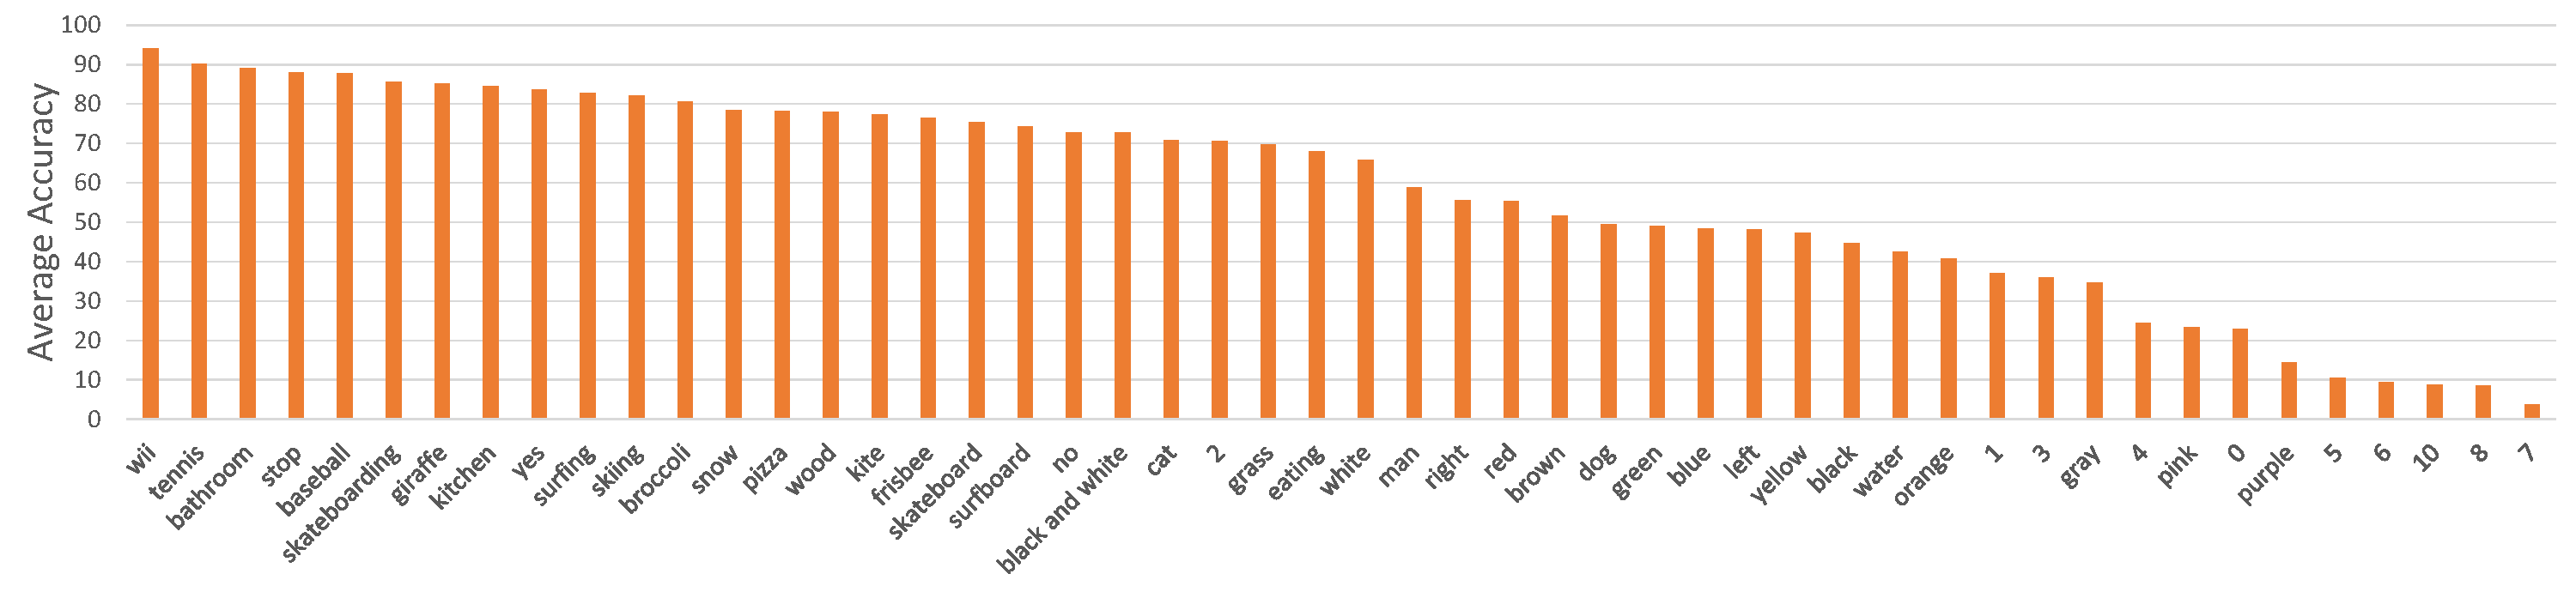
\includegraphics[width=1\linewidth]{figures/prob1_OpenEnded_val2014_sorted.pdf}
\centering
\caption{$\Pr\text{(system is correct } | \text{ answer)}$ for 50 most frequent ground truth answers on the VQA validation set (plot is sorted by accuracy, not frequency). System refers to our best model (deeper LSTM Q + norm I).}
\label{fig:prob_1}
%\vspace{\captionReduceBot}
\end{figure*}
\begin{figure*}[h]
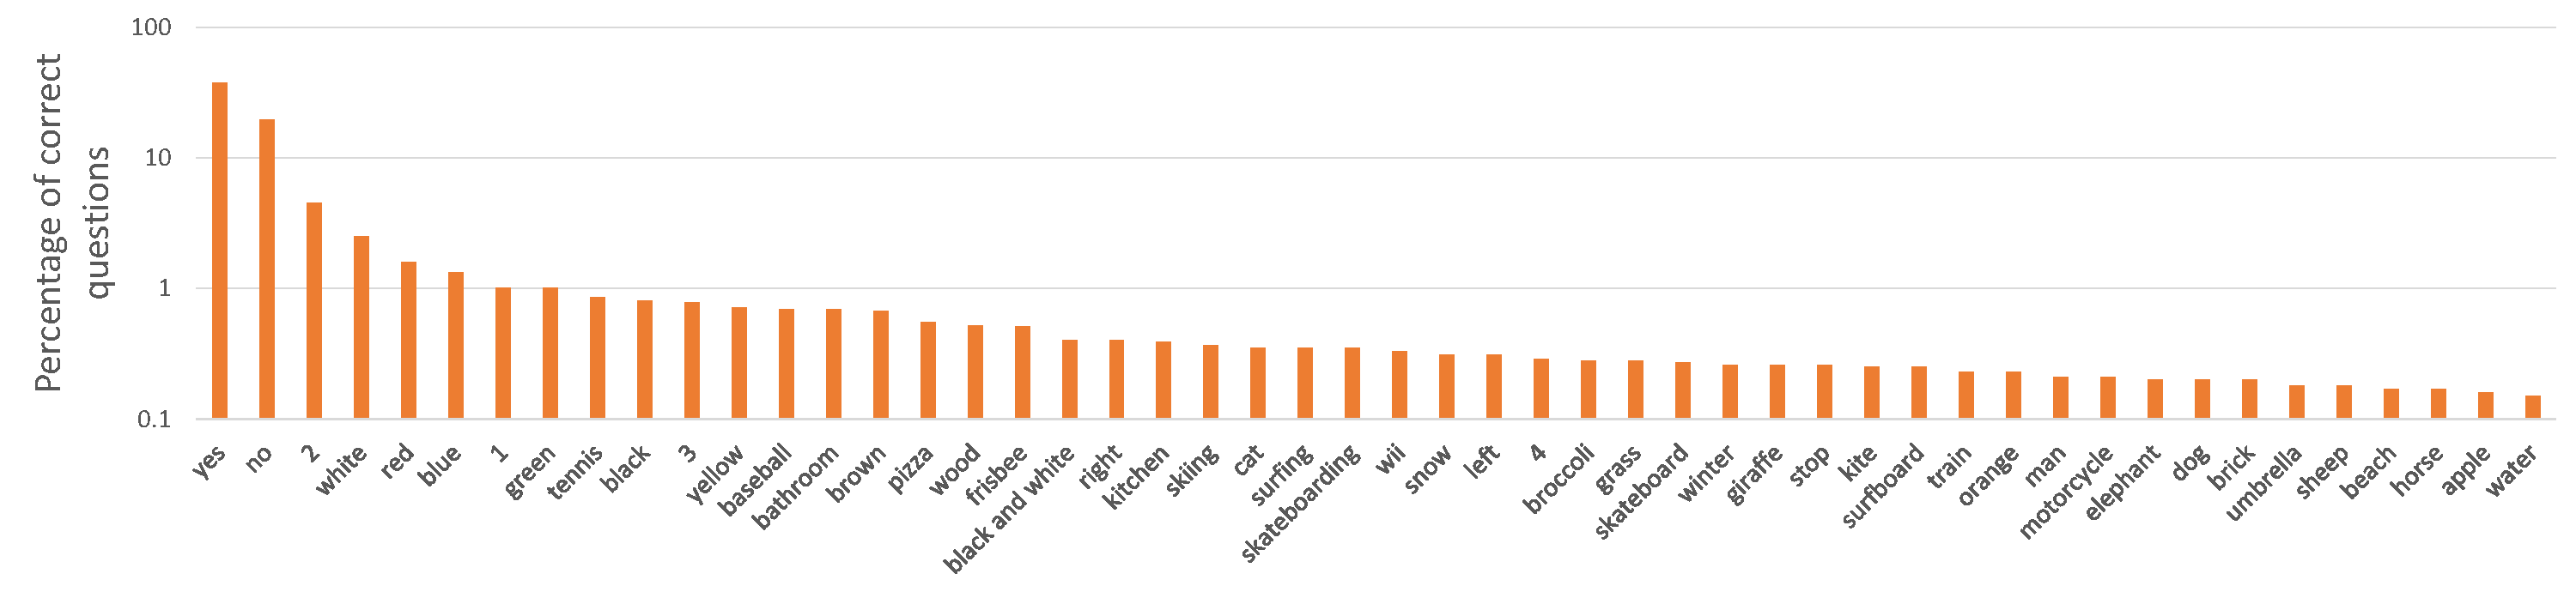
\includegraphics[width=1\linewidth]{figures/prob2_OpenEnded_val2014_100_logscale.pdf}
\centering
\caption{$\Pr\text{(answer } | \text{ system is correct)}$ for 50 most frequently predicted answers on the VQA validation set (plot is sorted by prediction frequency, not accuracy). System refers to our best model (deeper LSTM Q + norm I).}
\label{fig:prob_2}
%\vspace{\captionReduceBot}
\end{figure*}
\begin{figure}[h]
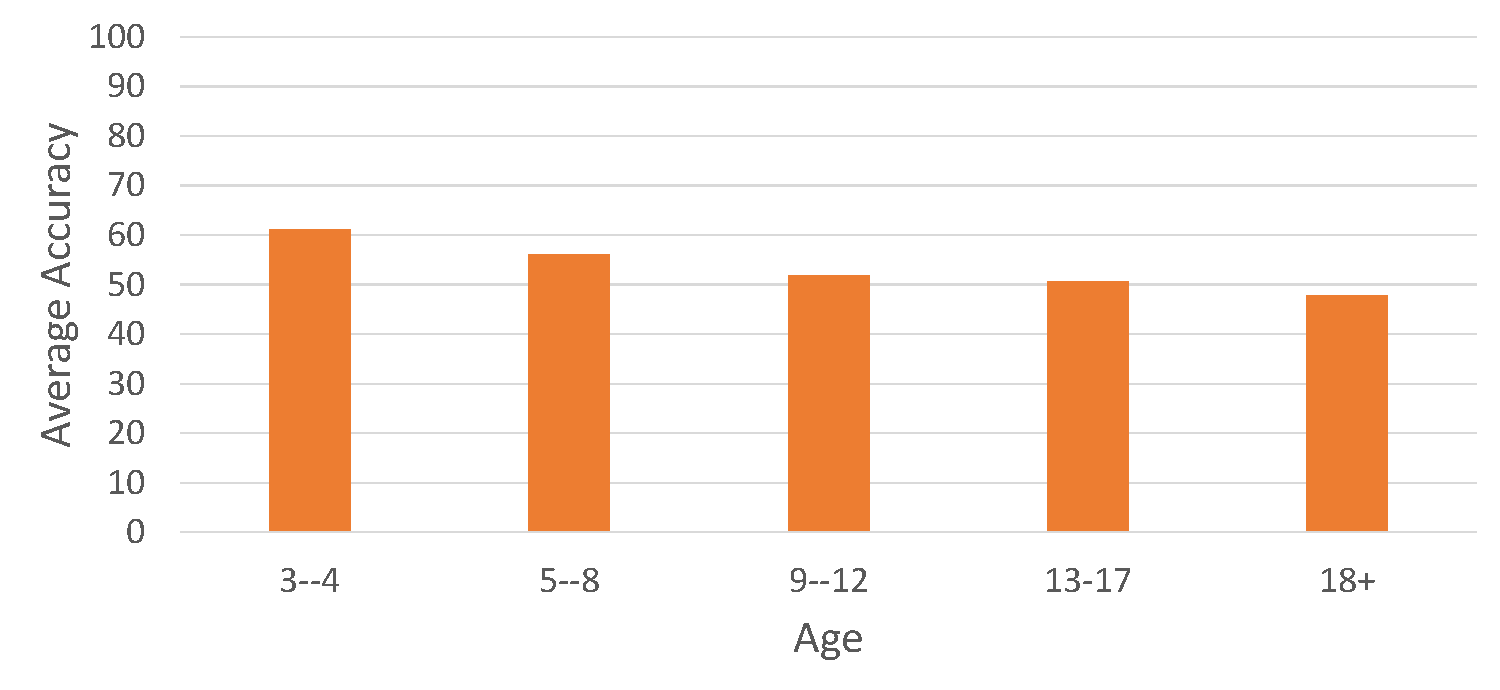
\includegraphics[width=1\linewidth]{figures/OpenEnded_val2014_predAgeDict2.pdf}
\centering
\caption{$\Pr\text{(system is correct } | \text{ age of question)}$ on the VQA validation set. System refers to our best model (deeper LSTM Q + norm I).}
\label{fig:age_1}
%\vspace{\captionReduceBot}
\end{figure}
\begin{figure}[h]
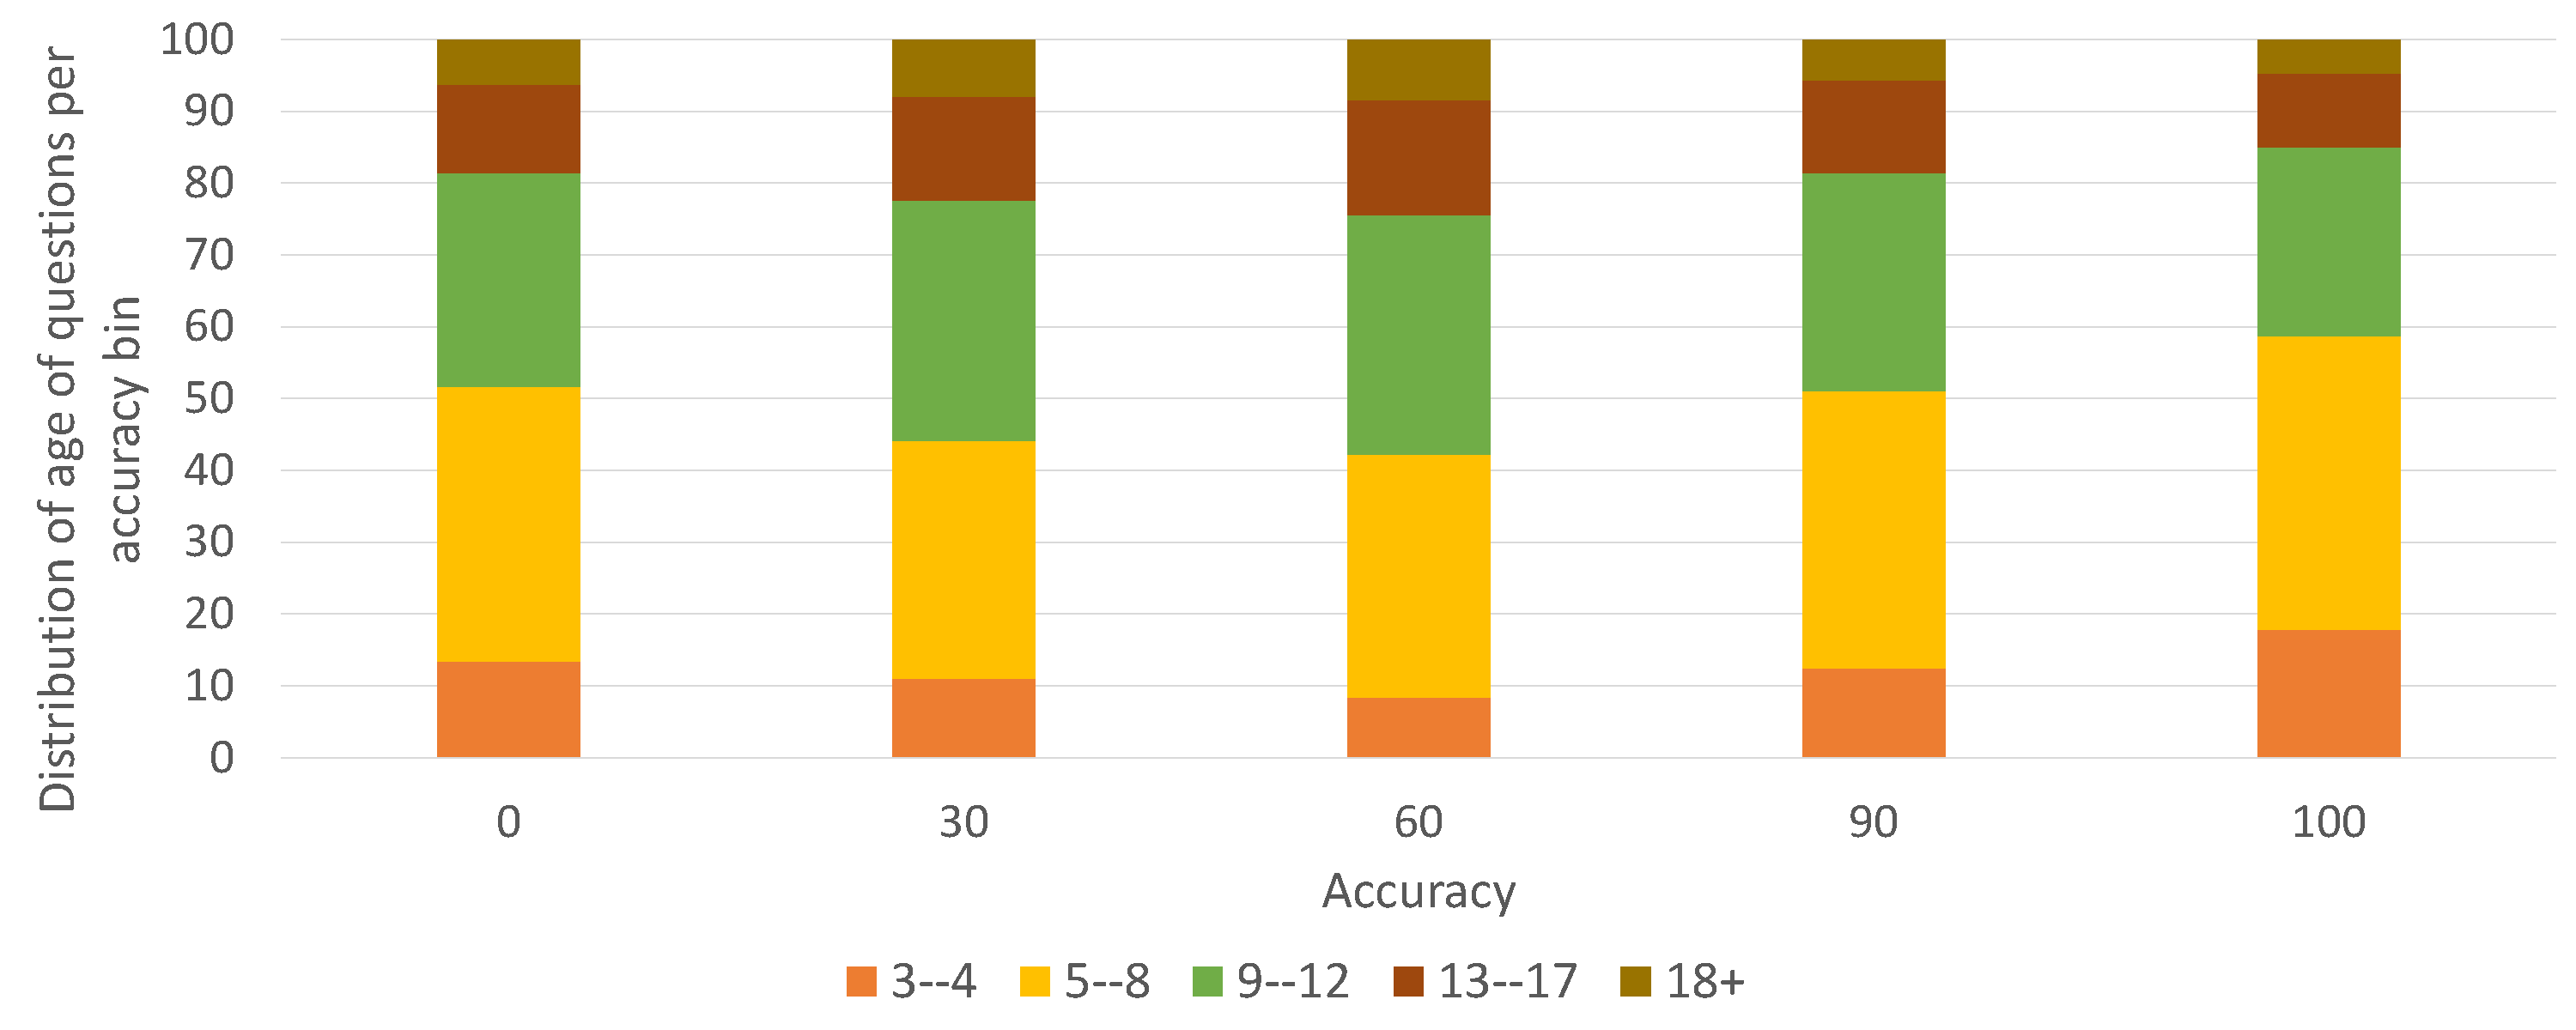
\includegraphics[width=1\linewidth]{figures/OpenEnded_val2014_predAgeDict1.pdf}
\centering
\caption{$\Pr\text{(age of question } | \text{ system is correct)}$ on the VQA validation set. System refers to our best model (deeper LSTM Q + norm I).}
\label{fig:age_2}
%\vspace{\captionReduceBot}
\end{figure}

\tableref{tab:abl_acc} shows the accuracy of different ablated versions of our best model (deeper LSTM Q + norm I) for both the open-ended and multiple-choice tasks on the VQA test-dev for real images. The different ablated versions are as follows --

\begin{compactenum}
\item \textbf{Without I Norm:} In this model, the activations from the last hidden layer of VGGNet~\cite{Simonyan14c} are not $\ell_2$-normalized. Comparing the accuracies in \tableref{tab:abl_acc} and \tableref{tab:acc}, we can see that $\ell_2$-normalization of image features boosts the performance by 0.16\% for open-ended task and by 0.24\% for multiple-choice task. 

\item \textbf{Concatenation:} In this model, the transformed image and LSTM embeddings are concatenated (instead of element-wise multiplied), resulting in doubling the number of parameters in the following fully-connected layer. Comparing the accuracies in \tableref{tab:abl_acc} and \tableref{tab:acc}, we can see that element-wise fusion performs better by 0.95\% for open-ended task and by 1.24\% for multiple-choice task.

\item \textbf{K = 500:} In this model, we use K = 500 most frequent answers as possible outputs. Comparing the accuracies in \tableref{tab:abl_acc} and \tableref{tab:acc}, we can see that K = 1000 performs better than K = 500 by 0.82\% for open-ended task and by 1.92\% for multiple-choice task.

\item \textbf{K = 2000:} In this model, we use K = 2000 most frequent answers as possible outputs. Comparing the accuracies in \tableref{tab:abl_acc} and \tableref{tab:acc}, we can see that K = 2000 performs better then K = 1000 by 0.40\% for open-ended task and by 1.16\% for multiple-choice task.

\item \textbf{Truncated Q Vocab $@$ 5:} In this model, the input vocabulary to the embedding layer (which encodes the question words) consists of only those question words which occur atleast 5 times in the training dataset, thus reducing the vocabulary size from 14770 (when all question words are used) to 5134 (65.24\% reduction). Remaining question words are replaced with UNK (unknown) tokens. Comparing the accuracies in \tableref{tab:abl_acc} and \tableref{tab:acc}, we can see that truncating the question vocabulary $@$ 5 performs better than using all questions words by 0.24\% for open-ended task and by 0.17\% for multiple-choice task.

\item \textbf{Truncated Q Vocab $@$ 11:} In this model, the input vocabulary to the embedding layer (which encodes the question words) consists of only those question words which occur atleast 11 times in the training dataset, thus reducing the vocabulary size from 14770 (when all question words are used) to 3561 (75.89\% reduction). Remaining question words are replaced with UNK (unknown) tokens. Comparing the accuracies in \tableref{tab:abl_acc} and \tableref{tab:acc}, we can see that truncating the question vocabulary $@$ 11 performs better than using all questions words by 0.06\% for open-ended task and by 0.02\% for multiple-choice task.

\item \textbf{Filtered Dataset:} We created a filtered version of the VQA train + val dataset in which we only keep the answers with subject confidence ``yes''. Also, we keep only those questions for which at least 50\% (5 out of 10) answers are annotated with subject confidence ``yes''. The resulting filtered dataset consists of 344600 questions, compared to 369861 questions in the original dataset, thus leading to only 6.83\% reduction in the size of the dataset. The filtered dataset has 8.77 answers per question on average. We did not filter the test set so that accuracies of the model trained on the filtered dataset can be compared with that of the model trained on the original dataset. The row ``Filtered Dataset'' in \tableref{tab:abl_acc} shows the performance of the deeper LSTM Q + norm I model when trained on the filtered dataset. Comparing these accuracies with the corresponding accuracies in \tableref{tab:acc}, we can see that the model trained on filtered version performs worse by 1.13\% for open-ended task and by 1.88\% for multiple-choice task.
\end{compactenum}

\begin{table}[t] \scriptsize
\setlength{\tabcolsep}{1.8pt}
\begin{center}
\begin{tabular}{@{} l  c  c  c  c  c  c c c@{}}
%\hline
\toprule
& \multicolumn{4}{c}{Open-Ended} & \multicolumn{4}{c}{Multiple-Choice} \\

\cmidrule[0.75pt](l){2-5}
\cmidrule[0.75pt](l){6-9}
 & All & Yes/No & Number & Other & All & Yes/No & Number & Other \\
%\hline
\midrule
Without I Norm & 57.59 & 80.41 & 36.63 & 42.84 & 62.46 & 80.43 & 38.10 & 52.62 \\
Concatenation & 56.80 & 78.49 & 35.08 & 43.19 & 61.46 & 78.52 & 36.43 & 52.54 \\
K = 500 & 56.93 & 80.61 & 36.24 & 41.39 & 60.78 & 80.64 & 37.44 & 49.10 \\
K = 2000 & 58.15 & 80.56 & 37.04 & 43.79 & 63.86 & 80.59 & 38.97 & 55.20 \\
Truncated Q Vocab $@$ 5 & 57.99 & 80.67 & 36.99 & 43.38 & 62.87 & 80.71 & 38.22 & 53.20\\
Truncated Q Vocab $@$ 11 & 57.81 & 80.42 & 36.97 & 43.22 & 62.72 & 80.45 & 38.30 & 53.09\\
Filtered Dataset & 56.62 & 80.19 & 37.48 & 40.95 & 60.82 & 80.19 & 37.48 & 49.57 \\
\bottomrule
\end{tabular}	
\caption{Accuracy of ablated versions of our best model (deeper LSTM Q + norm I) for the open-ended and multiple-choice tasks on the VQA test-dev for real images. 
Q = Question, I = Image. 
See text for details.
}
%\vspace{-10pt}
\label{tab:abl_acc}
\end{center}
\end{table}
%\vspace{\sectionReduceTop}
\section{VQA Challenge and Workshop}
\label{sec:challenge}
%\vspace{\sectionReduceBot}

%We have collected questions for \textcolor{red}{200k} MS COCO images. \aishwarya{Do we still need to keep next line?} However, to increase the diversity of the dataset, we are also considering the addition of images from other sources. The use of more complex and diverse abstract scenes could also open up new application areas.
We have set up an evaluation server\footnote{\url{http://visualqa.org/challenge.html}} where results may be uploaded for the test set and it returns an accuracy breakdown. We are organizing an annual challenge and workshop to facilitate systematic progress in this area; the first instance of the workshop will be held at CVPR 2016\footnote{\url{http://www.visualqa.org/workshop.html}}. We suggest that papers reporting results on the VQA dataset --

\begin{compactenum}

\item Report test-standard accuracies, which can be calculated using either of the non-test-dev phases, i.e., ``test2015'' or ``Challenge test2015'' on the following links: [\href{https://www.codalab.org/competitions/6961}{oe-real} $|$ \href{https://www.codalab.org/competitions/6981}{oe-abstract} $|$ \href{https://www.codalab.org/competitions/6971}{mc-real} $|$ \href{https://www.codalab.org/competitions/6991}{mc-abstract}].

\item Compare their test-standard accuracies with those on the corresponding test2015 leaderboards [\href{http://www.visualqa.org/roe.html}{oe-real-leaderboard} $|$ \href{http://www.visualqa.org/aoe.html}{oe-abstract-leaderboard} $|$ \href{http://www.visualqa.org/rmc.html}{mc-real-leaderboard} $|$ \href{http://www.visualqa.org/amc.html}{mc-abstract-leaderboard}].
%\item Compare their test-standard accuracies with those on the corresponding test2015 leaderboards [\href{https://competitions.codalab.org/competitions/6961\#results}{oe-real-leaderboard} $|$ \href{https://www.codalab.org/competitions/6981\#results}{oe-abstract-leaderboard} $|$ \href{https://www.codalab.org/competitions/6971\#results}{mc-real-leaderboard} $|$ \href{https://www.codalab.org/competitions/6991\#results}{mc-abstract-leaderboard}]. 
%We are working on building a COCO-style leaderboard which can provide you with appropriate references to cite, but in the meantime, please use the information (such as username, teamname, \etc) from the test2015 leaderboards to refer to other entries.

\end{compactenum}

For more details, please see the challenge page\footnote{\url{http://visualqa.org/challenge.html}}. Screenshots of leaderboards for open-ended-real and multiple-choice-real are shown in \figref{fig:leaderboard-oe}.
% \figref{fig:leaderboard-real-oe} and \figref{fig:leaderboard-real-mc} respectively.
We also compare the test-standard accuracies of our best model (deeper LSTM Q + norm I) for both open-ended and multiple-choice tasks (real images) with other entries (as of \today) on the corresponding leaderboards in \tableref{tab:comparison_leaderboard}.

\begin{table}[t] \scriptsize
\setlength{\tabcolsep}{1.8pt}
\begin{center}
\begin{tabular}{@{} l  c  c  c  c  c  c c c@{}}
%\hline
\toprule
& \multicolumn{4}{c}{Open-Ended} & \multicolumn{4}{c}{ Multiple-Choice} \\

\cmidrule[0.75pt](l){2-5}
\cmidrule[0.75pt](l){6-9}
 & All & Yes/No & Number & Other & All & Yes/No & Number & Other \\
%\hline
\midrule
snubi-naverlabs & 60.60 & 82.23 & 38.22 & 46.99 
& 64.95 & 82.25 & 39.56 & 55.68 \\
MM\_PaloAlto & 60.36 & 80.43 & 36.82 & 48.33 
& -- & -- & -- & -- \\
LV-NUS & 59.54 & 81.34 & 35.67 & 46.10 
& 64.18 & 81.25 & 38.30 & 55.20 \\
ACVT\_Adelaide & 59.44 & 81.07 & 37.12 & 45.83 
& -- & -- & -- & --\\
global\_vision & 58.43 & 78.24 & 36.27 & 46.32 
& -- & -- & -- & --\\
deeper LSTM Q + norm I & 58.16 & 80.56 & 36.53 & 43.73 
& 63.09 & 80.59 & 37.70 & 53.64\\
iBOWIMG	 & -- & -- & -- & --
& 61.97 & 76.86 & 37.30 & 54.60\\
\bottomrule
\end{tabular}	
\caption{Test-standard accuracy of our best model (deeper LSTM Q + norm I) compared to test-standard accuracies of other entries for the open-ended and multiple-choice tasks in the respective VQA Real Image Challenge leaderboards (as of \today).}
%\vspace{-5pt}
\label{tab:comparison_leaderboard}
\end{center}
\end{table}

\begin{figure*}[h]
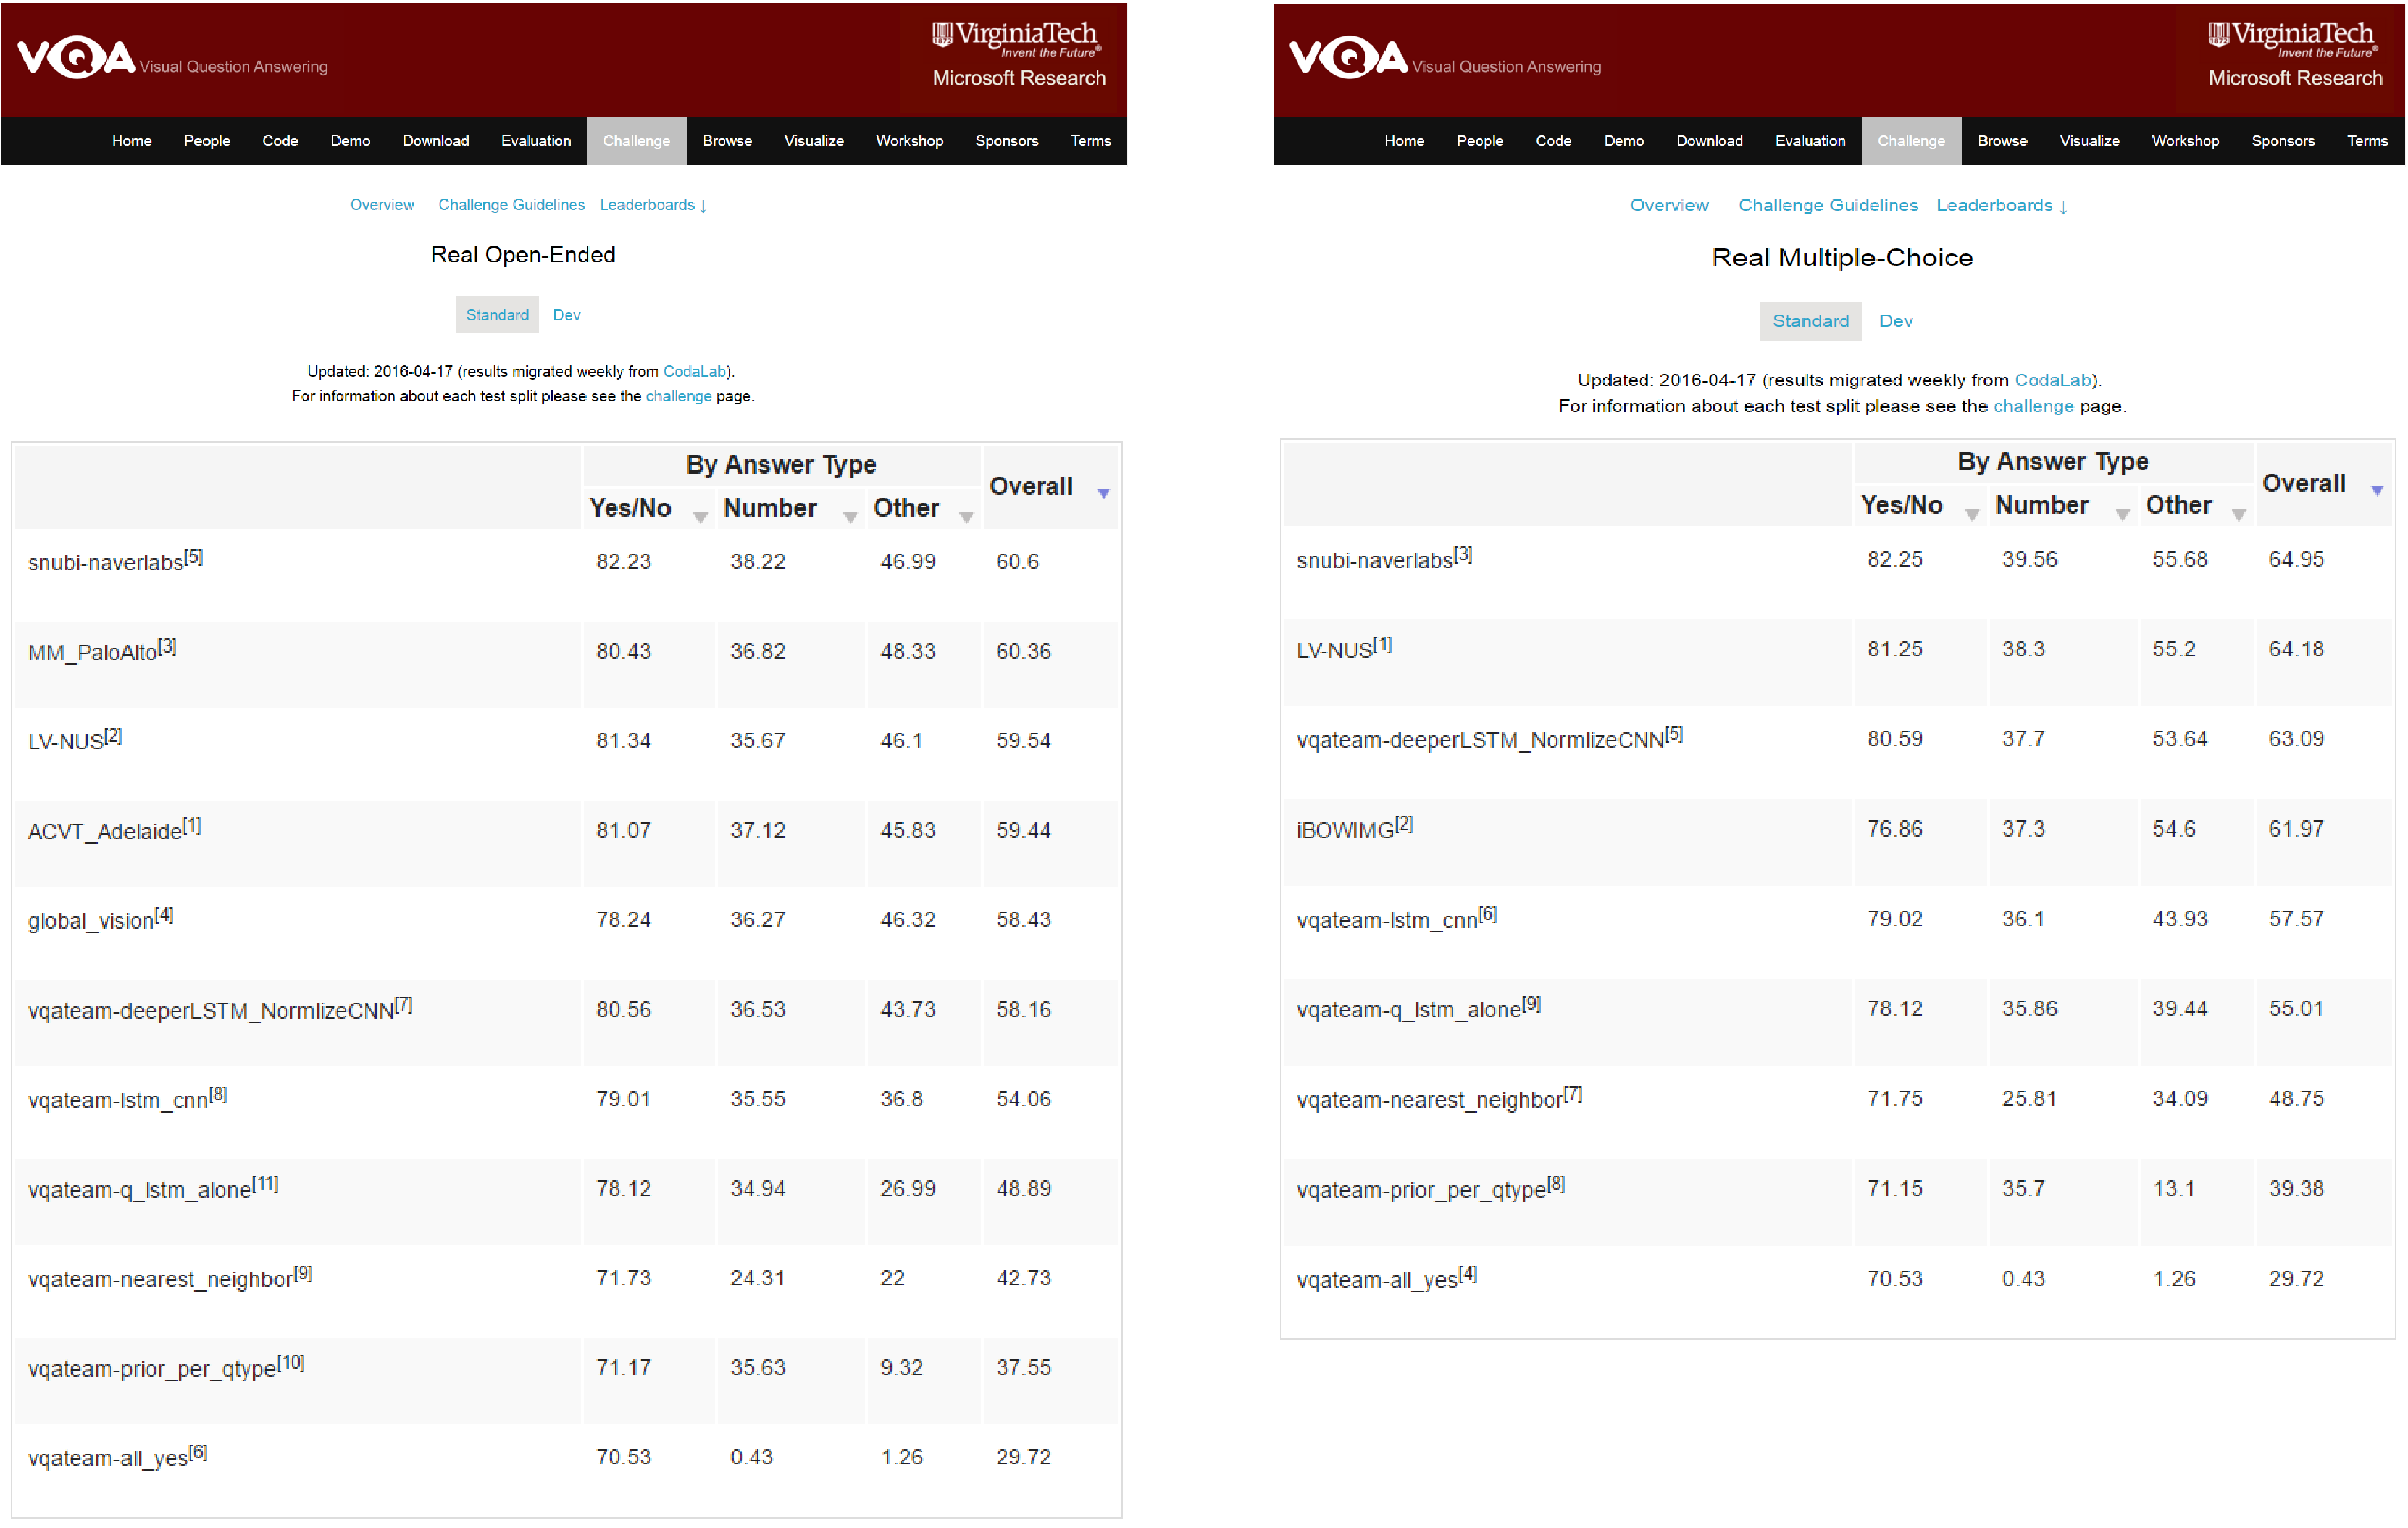
\includegraphics[width=1\linewidth]{figures/real-screenshot.pdf}
\centering
\caption{Leaderboard showing test-standard accuracies for VQA Real Image Challenge (Open-Ended) on left and leaderboard showing test-standard accuracies for VQA Real Image Challenge (Multiple-Choice) on right (snapshot from \today).}
\label{fig:leaderboard-oe}
%\vspace{\captionReduceBot}
\end{figure*}

%\begin{figure}[h!]
%\includegraphics[width=1\linewidth]{figures/real-oe-screenshot.pdf}
%\centering
%\caption{Leaderboard showing test-standard accuracies for VQA Real Image Challenge (Open-Ended) (snapshot from \today).}
%\label{fig:leaderboard-real-oe}
%%\vspace{\captionReduceBot}
%\end{figure}
%\begin{figure}[h!]
%\includegraphics[width=1\linewidth]{figures/real-mc-screenshot.pdf}
%\centering
%\caption{Leaderboard showing test-standard accuracies for VQA Real Image Challenge (Multiple-Choice) (snapshot from \today).}
%\label{fig:leaderboard-real-mc}
%%\vspace{\captionReduceBot}
%\end{figure} 
\section{Discussion}
\label{sec:discussion}

The accuracy on the CKP set shows that the chosen approach is robust, misclassification usually occurs on pictures which are the first few instances of an emotion sequence. Often a neutral facial expression is depicted in those frames. Thus those misclassifications are not necessarily an error in the approach, but in the data selection. Other than that no major problem could be detected. The emotion \textit{Surprise} is often confused with \textit{Disgust} with a rate of 0.045\% which is the highest. Of those images, where an emotion is present, only few are wrongly classified.\\ 


As there is no consent for the misclassified images, they cannot be depicted here. However some unique names are provided. \\
Image S119\_001\_00000010 is classified as \textit{Fear} while the annotated emotion corresponds to \textit{Surprise}. The image depicts a person with a wide open mouth and open eyes. Pictures representing \textit{Surprise} are often very similar, since the persons also have wide open mouths and eyes. In image S032\_004\_00000014 the targeted label \textit{Fear} is confused with \textit{Anger}. While the mouth region in pictures with \textit{Anger} differ, the eye regions are alike, since in both situations the eyes and eyebrows are contracted.\\
Similar effects are experienced when dealing with the MMI Dataset. Since the first two frames are discarded most pictures with neutral positions are excluded. In few images a neutral position can still be found which gives rise to errors. For the same reason as the CKP set images will not be displayed. Due to the approach to extract images of the videos, a unique identifier for the misclassified image cannot be provided.\\
The top confusions are observed for \textit{Fear} and \textit{Surprise} with a rate of 0.0159\% where \textit{Fear} is wrongly misclassified as \textit{Surprise}. Session 1937 shows a woman displaying \textit{Fear} but it is classified as \textit{Surprise}. Both share common features like similar eye and mouth movement. In both emotions, participants move the head slightly backwards. This can be identified by wrinkled skin. The second most confusion rate, \textit{Surprise} being mistaken as \textit{Sadness}, is mostly based on neutral position images. Although the first two images are not used, some selected frames still do not contain an emotion. In Session 1985 \textit{Surprise} is being mistaken as \textit{Sadness}. The image depicts a man with his mouth being slightly curved, making him look sad.\\

DeXpression extracts features and uses them to classify images, but in very few cases the emotions are confused. This happens, as discussed, usually in pictures depicting no emotion. DeXpression performs very well on both tested sets, if an emotion is present.



%\clearpage
%\columnbreak
\section*{Appendix Overview}
%%%%%%%%%%%%%%%%%%%%%%%%%%%%%%%%%%%%%%%%%%%%%%%%%%%%%%%%%%%
% Body
%%%%%%%%%%%%%%%%%%%%%%%%%%%%%%%%%%%%%%%%%%%%%%%%%%%%%%%%%%%
In the appendix, we provide:
 \begin{enumerate}[I]
\setlength{\itemsep}{1pt}
  \setlength{\parskip}{0pt}
  \setlength{\parsep}{0pt}
 \item - Additional analysis comparing captions and Q\&A data
 \item - Qualitative visualizations for ``What is'' questions
 \item - Human accuracy on multiple-choice questions
 \item - \change{Details on VQA baselines}
  \item - \changenew{``Age'' and ``Commonsense'' of our model}
 \item - Details on the abstract scene dataset
 \item - User interfaces used to collect the dataset
 \item - List of the top answers in the dataset
 \item - Additional examples from the VQA dataset
 \end{enumerate}

 \begin{comment}
 an update on the dataset collection in \secref{subsec:dataset_stats}, show the interfaces that were used on Amazon Mechanical Turk (AMT) in \secref{subsec:interfaces}, and show additional example questions and answers from our VQA dataset in \secref{subsec:more_examples}. Then we provide some further analysis of the VQA dataset in \secref{sec:analysis}. In addition, \secref{sec:analysis} also shows the new results of a recent experiment to estimate inter-human agreement for multiple-choice questions.
\end{comment}


%\section{VQA Dataset Collection Progress}
%\label{sec:dataset_stats}
%%%%%%%%%%%%%%%%%%%%%%%%%%%%%%%%%%%%%%%%%%%%%%%%%%%%%%%%%%%%
%
%As of this submission, the VQA dataset has 123,285 images, 215,150 questions, and a total of 430,920 answers (including answers provided by workers while looking at the image and without looking at the image; recall that the latter become options in the multiple-choice question format) for real images from the MS COCO dataset~\cite{coco}. Since the main submission, our primary focus was collecting more questions for more real images, thus the abstract scene dataset is the same size as reported in the main document.
\section*{Appendix I: Captions \vs Questions}
\label{sec:cap_vs_q}
Do questions and answers provide further information about the visual world beyond that captured by captions? One method for determining whether the information captured by questions \& answers is different from the information captured by captions is to measure some of the differences in the word distributions from the two datasets. We cast this comparison in terms of nouns, verbs, and adjectives by extracting all words from the caption data \change{(MS COCO captions for real images and captions collected by us for abstract scenes)} using the Stanford part-of-speech (POS)\footnote{Noun tags begin with NN, verb tags begin with VB, adjective tags begin with JJ, and prepositions are tagged as IN.} tagger~\cite{StanfordPOS}.  We normalize the word frequencies from captions, questions, and answers per image, and compare captions \vs questions and answers combined.  Using a Kolmogorov-Smirnov test to determine whether the underlying distributions of the two datasets differ, we find a significant difference for all three parts of speech (p $<$ .001) \change{for both real images and abstract scenes}. This helps motivate the VQA task as a way to learn information about visual scenes; although both captions and questions \& answers provide information about the visual world, they do it from different perspectives, with different underlying biases \cite{GordonVanDurme13}, and can function as complementary to one another.  %This also may help explain why performance when answering questions is significantly worse when only using the captions and not the image (\ie, Table 1 in the main paper).

%To visualize the differences between the data sets, we again use the Stanford POS tagger to tag words as nouns (NN*), verbs (VB*), adjectives (JJ*), and prepositions (IN), normalizing counts per image, and extracting the top 500 words for each.
We illustrate the similarities and differences between the word distributions in captions vs. questions \& answers as Venn-style word clouds \cite{CoppersmithKelly14} with size indicating the normalized count -- \figref{fig:noun_cloud_real} (nouns), \figref{fig:verb_cloud_real} (verbs), and \figref{fig:adj_cloud_real} (adjectives) \change{for real images and \figref{fig:noun_cloud_abs} (nouns), \figref{fig:verb_cloud_abs} (verbs), and \figref{fig:adj_cloud_abs} (adjectives) for abstract scenes}.\footnote{Visualization created using \url{http://worditout.com/}.}  The left side shows the top words in questions \& answers, the right the top words in captions, and the center the words common to both, with size indicating the harmonic mean of the counts.

We see that adjectives in captions capture some clearly visual properties discussed in previous work on vision to language \cite{MitchellEtAl13}, such as material and pattern, while the questions \& answers have more adjectives that capture what is usual (\eg, \change{``dominant'', ``approximate'', ``higher''}) and other kinds of commonsense properties (\eg, \change{``edible'', ``possible'', ``unsafe'', ``acceptable''}).  Interestingly, we see that question \& answer nouns capture information about \change{``ethnicity'' and ``hairstyle''}, while caption nouns capture information about \change{pluralized visible objects (\eg, ``cellphones'', ``daughters'') and groups (\eg, ``trio'', ``some''), among other differences.} ``Man'' and ``people'' are common in both captions and questions \& answers.

One key piece to understanding the visual world is understanding spatial relationships, and so we additionally extract spatial prepositions and plot their proportions in the captions \vs~the questions \& answers data in \figref{fig:spatial_prepositions} (left) for real images and \figref{fig:spatial_prepositions} (right) for abstract scenes.  We see that questions \& answers have a higher proportion of specific spatial relations (\ie, ``in'', ``on'') compared to captions, which have a higher proportion of general spatial relations (\ie, ``with'', \change{``near''}).

\begin{figure*}
\centering
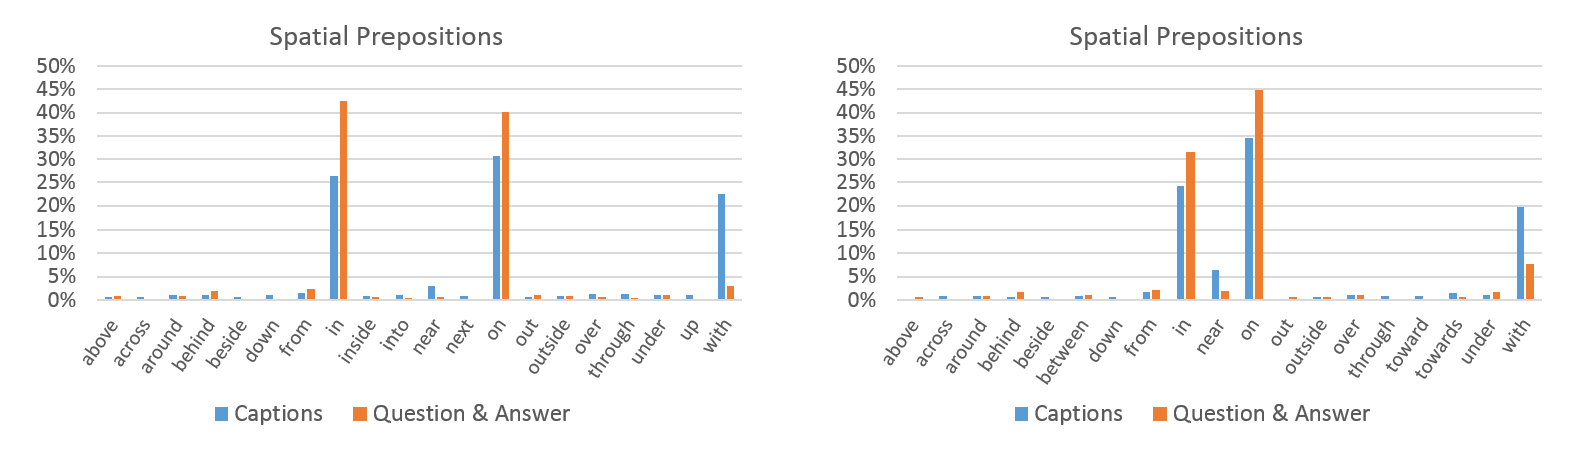
\includegraphics[width=\linewidth]{figures/spatial_prepositions.pdf}
\caption{Proportions of spatial prepositions in the captions and question \& answers for real images (left) and abstract scenes (right).}
%\vspace{-5pt}
\label{fig:spatial_prepositions}
\end{figure*}

%\begin{figure}
%\centering
%\includegraphics[width=\linewidth]{figures/coco_captions_vs_qa-spatial_prepositions.pdf}
%\caption{Proportions of spatial prepositions in the captions and question \& answers \change{for real images}.}
%%\vspace{-5pt}
%\label{fig:spatial_prepositions_real}
%\end{figure}

%\begin{figure}
%\centering
%\includegraphics[width=\linewidth]{figures/abstract_captions_vs_qa-spatial_prepositions.pdf}
%\caption{Proportions of spatial prepositions in the captions and question \& answers \change{for abstract scenes}.}
%%\vspace{-5pt}
%\label{fig:spatial_prepositions_abs}
%\end{figure}

\begin{figure*}
\centering
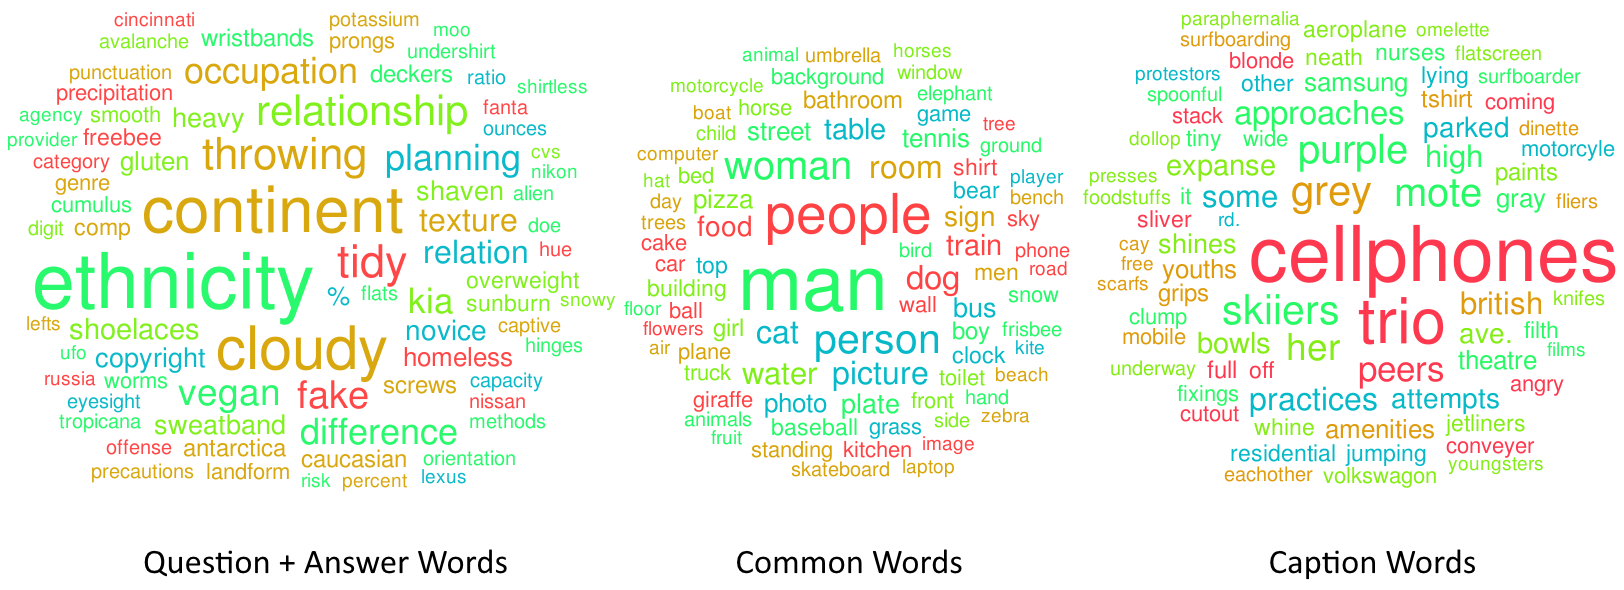
\includegraphics[width=0.9\linewidth]{figures/coco_nouns.png}
\caption{Venn-style word clouds \cite{CoppersmithKelly14} for nouns with size indicating the normalized count \change{for real images}.}
%\vspace{-5pt}
\label{fig:noun_cloud_real}
%\setlength{\belowcaptionskip}{-10pt}
\end{figure*}

\begin{figure*}
\centering
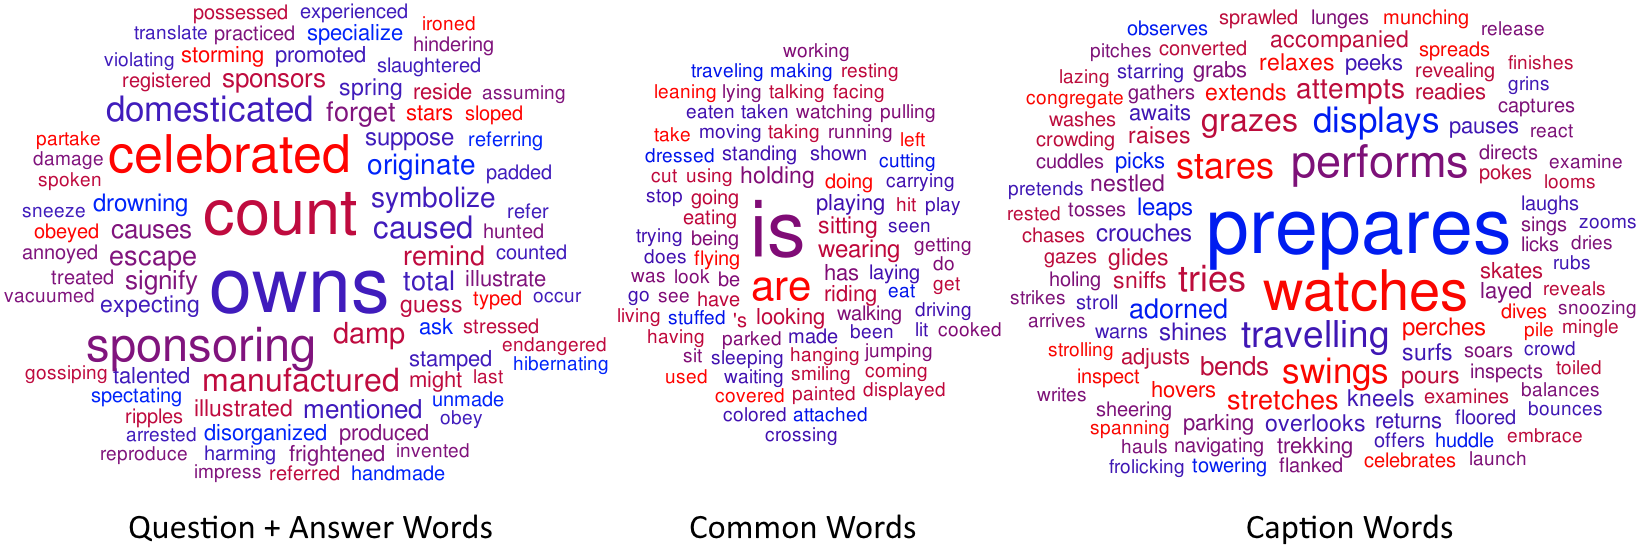
\includegraphics[width=0.9\linewidth]{figures/coco_verbs.png}
\caption{Venn-style word clouds \cite{CoppersmithKelly14} for verbs with size indicating the normalized count \change{for real images}.}
%\vspace{-5pt}
\label{fig:verb_cloud_real}
%\setlength{\belowcaptionskip}{-10pt}
\end{figure*}

\begin{figure*}
\centering
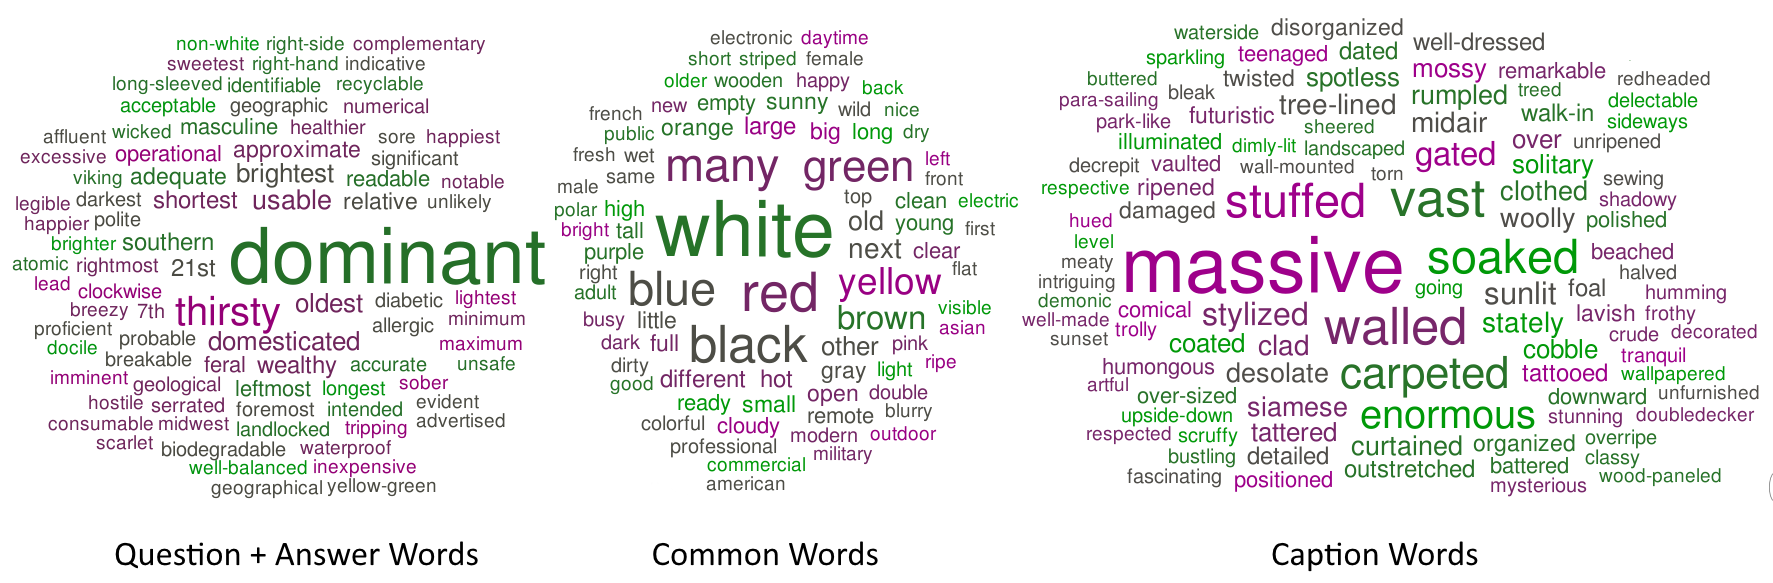
\includegraphics[width=0.9\linewidth]{figures/coco_adjectives.png}
\caption{Venn-style word clouds \cite{CoppersmithKelly14} for adjectives with size indicating the normalized count \change{for real images}.}
%\vspace{-5pt}
\label{fig:adj_cloud_real}
%\setlength{\belowcaptionskip}{-10pt}
\end{figure*}
\clearpage

\begin{figure*}
\centering
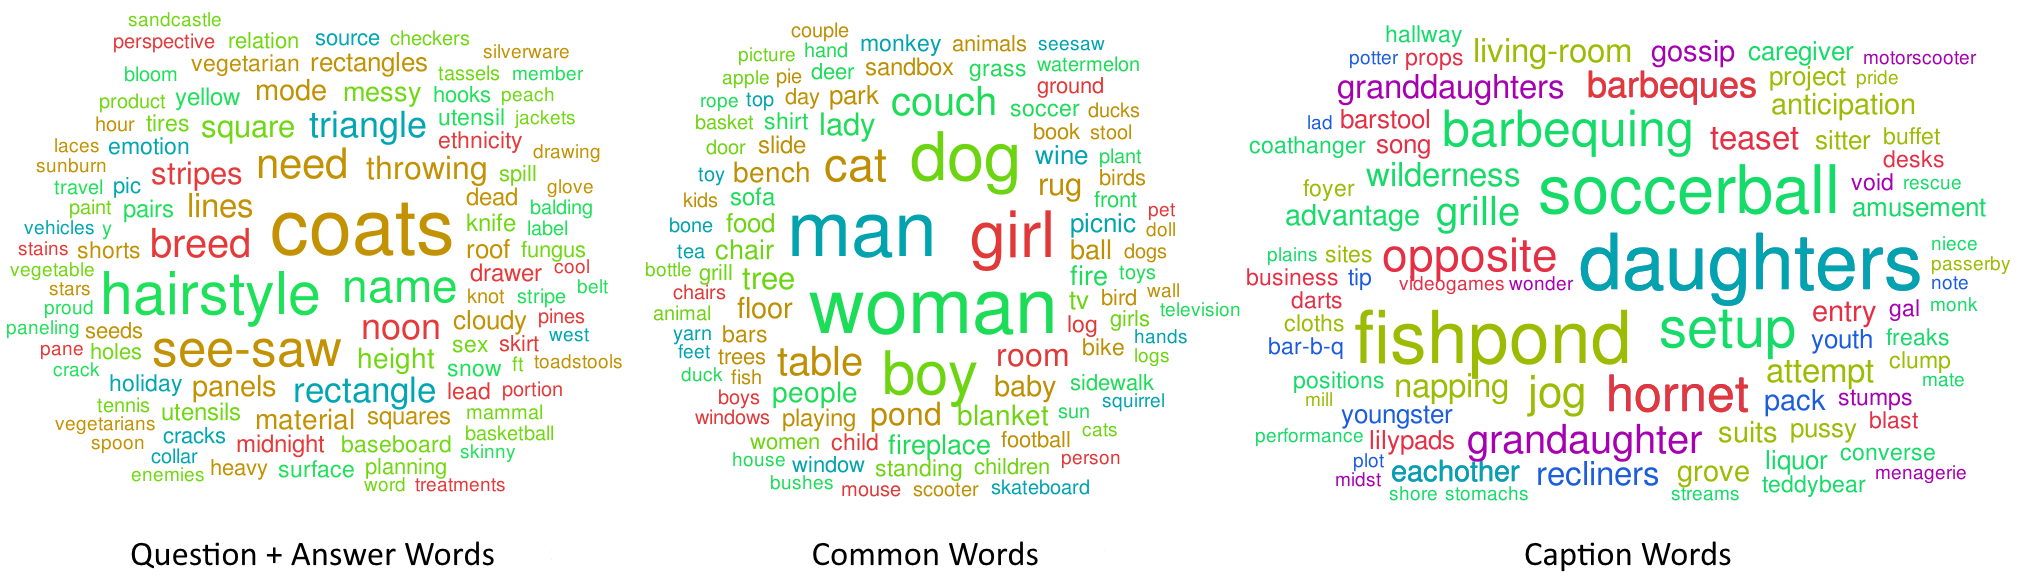
\includegraphics[width=0.9\linewidth]{figures/abstract_nouns.png}
\caption{Venn-style word clouds \cite{CoppersmithKelly14} for nouns with size indicating the normalized count \change{for abstract scenes}.}
%\vspace{-5pt}
\label{fig:noun_cloud_abs}
%\setlength{\belowcaptionskip}{-10pt}
\end{figure*}

\begin{figure*}
\centering
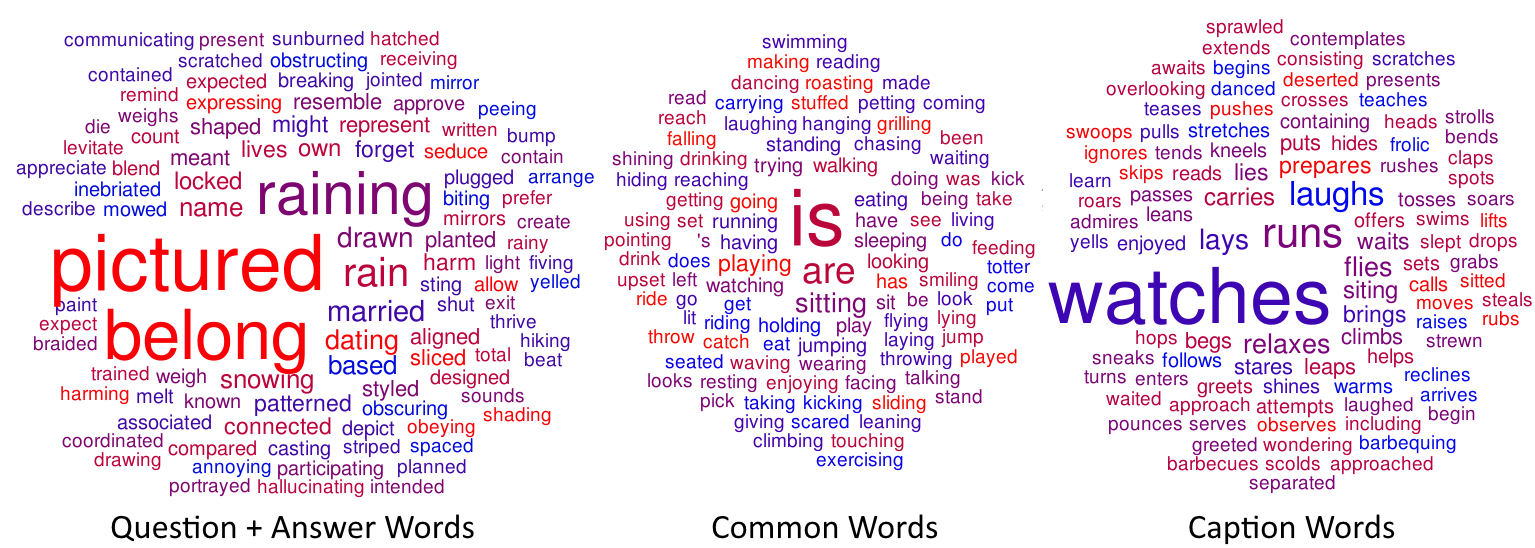
\includegraphics[width=0.9\linewidth]{figures/abstract_verbs.png}
\caption{Venn-style word clouds \cite{CoppersmithKelly14} for verbs with size indicating the normalized count \change{for abstract scenes}.}
%\vspace{-5pt}
\label{fig:verb_cloud_abs}
%\setlength{\belowcaptionskip}{-10pt}
\end{figure*}

\begin{figure*}
\centering
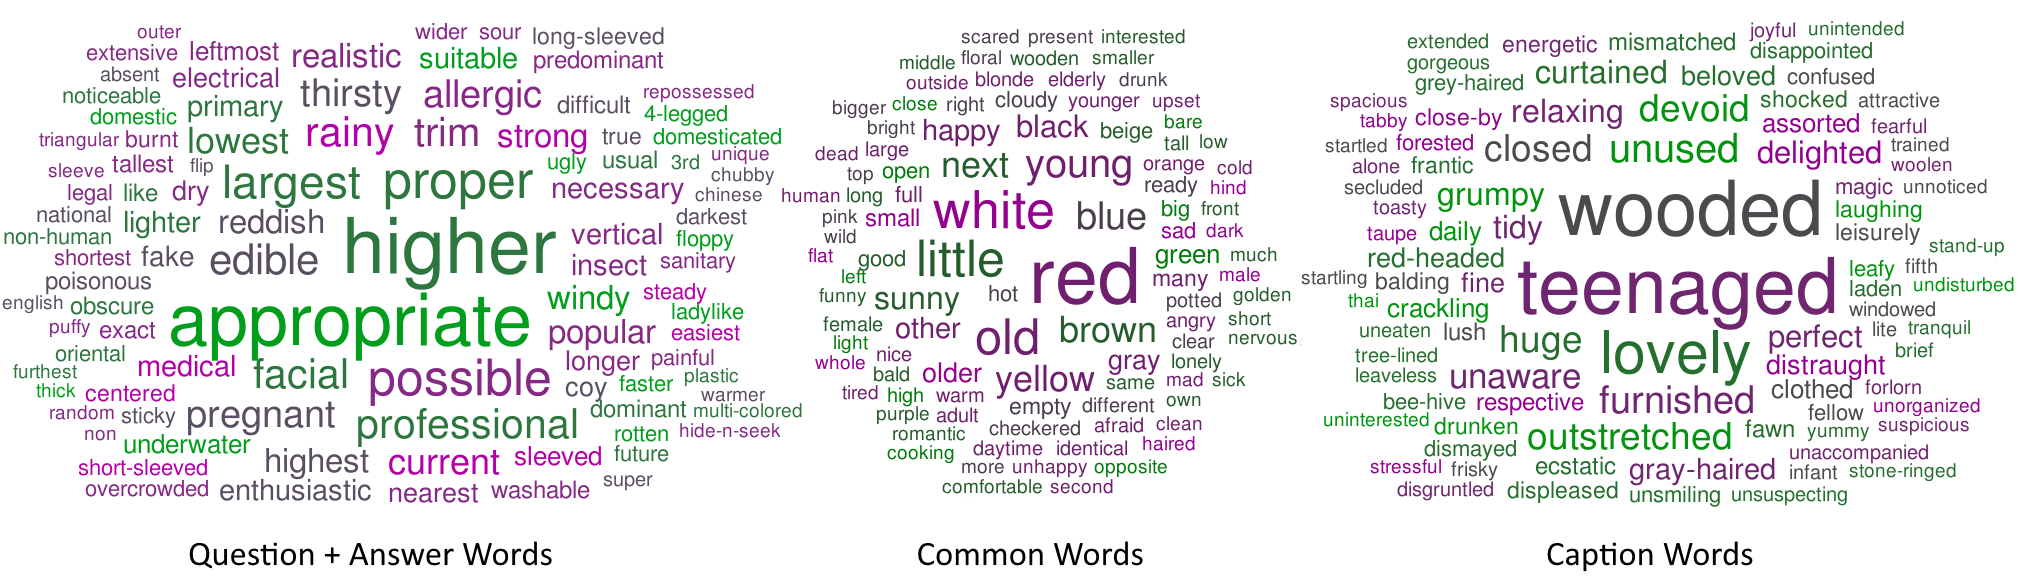
\includegraphics[width=0.9\linewidth]{figures/abstract_adjectives.png}
\caption{Venn-style word clouds \cite{CoppersmithKelly14} for adjectives with size indicating the normalized count \change{for abstract scenes}.}
%\vspace{-5pt}
\label{fig:adj_cloud_abs}
%\setlength{\belowcaptionskip}{-10pt}
\end{figure*}
\clearpage

\begin{figure*}
\centering
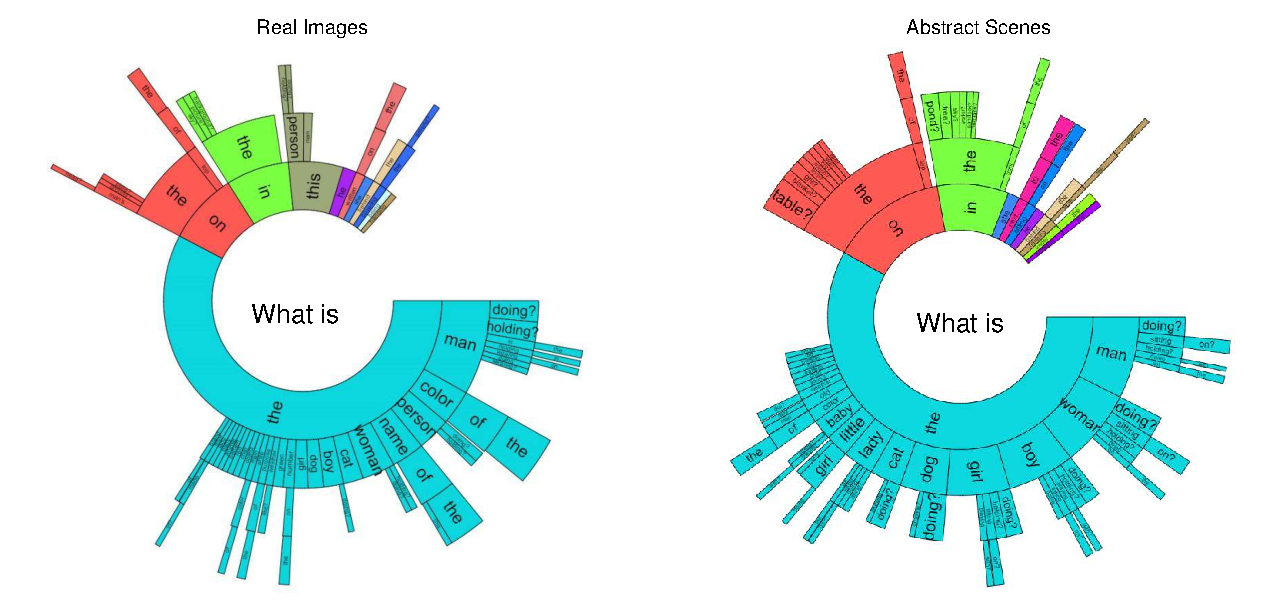
\includegraphics[width=0.95\linewidth]{figures/WhatIsQuestionTypes_mod_compressed.pdf}
\caption{\change{Distribution of questions starting with ``What is'' by their first five words for a random sample of 60K questions for real images (left) and all questions for abstract scenes (right). The ordering of the words starts towards the center and radiates outwards. The arc length is proportional to the number of questions containing the word. White areas are words with contributions too small to show.}}
%\vspace{-5pt}
\label{fig:WhatIsDistribution}
%\setlength{\belowcaptionskip}{-10pt}
\end{figure*}
\begin{figure*}
\centering
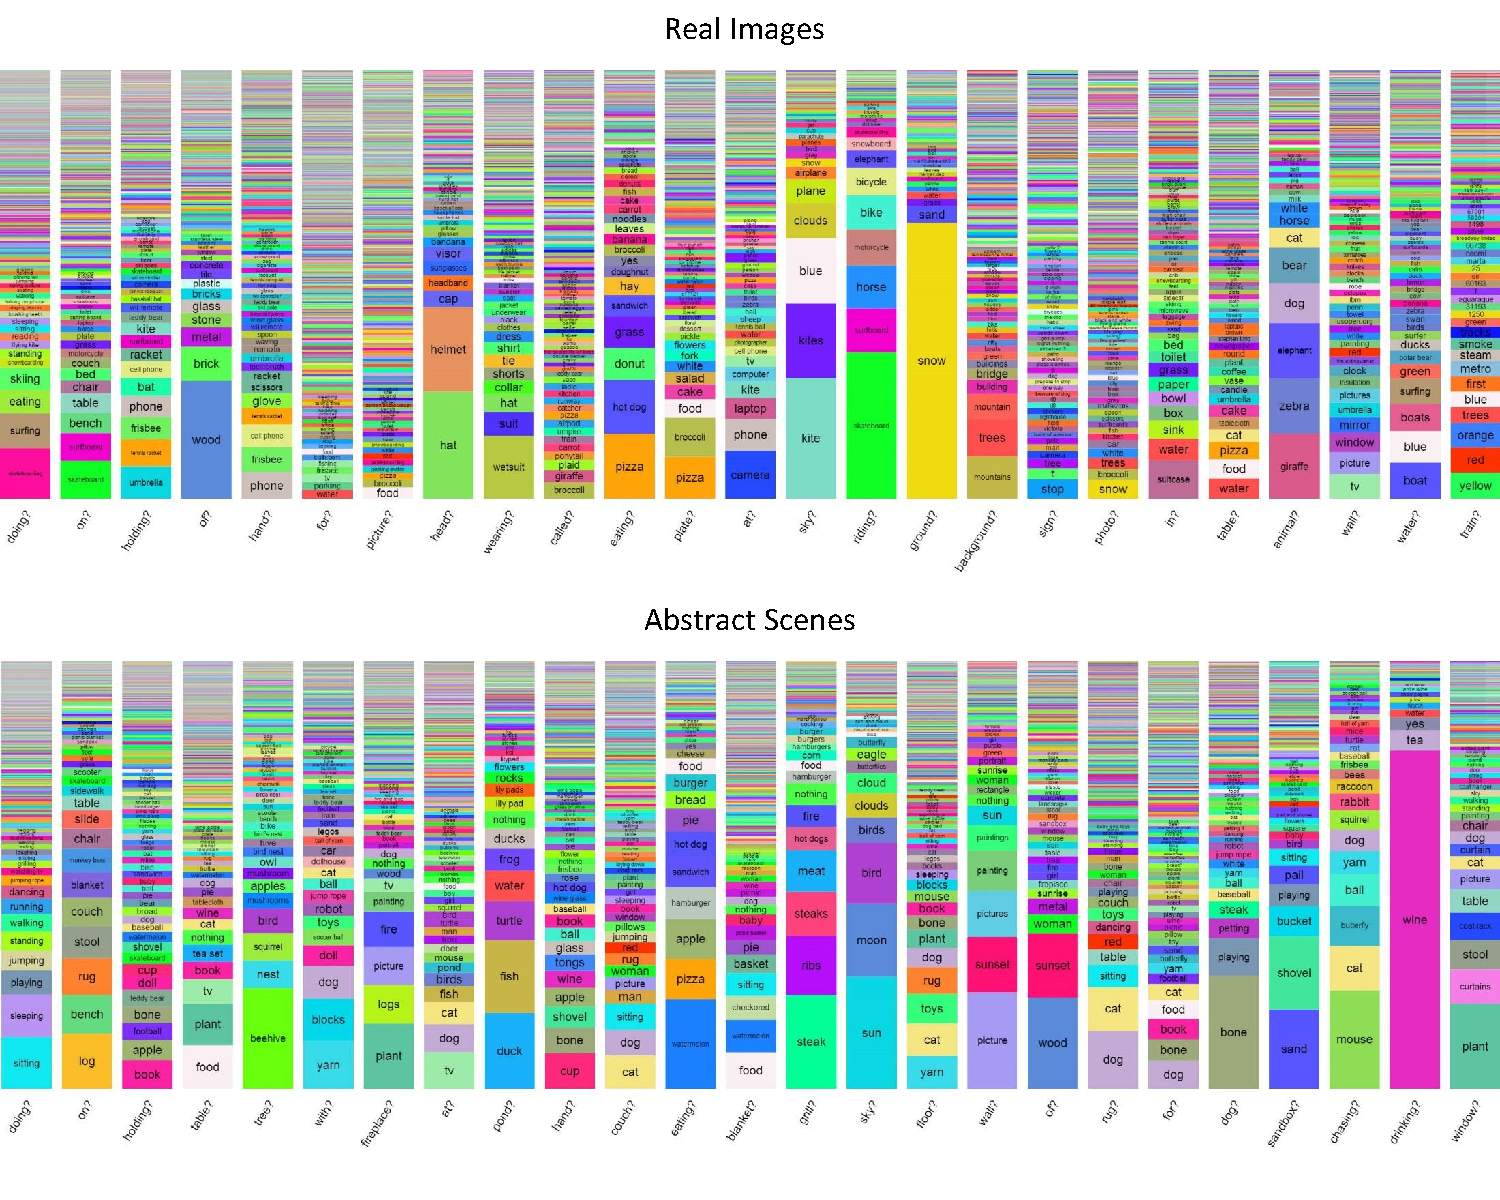
\includegraphics[width=0.95\linewidth]{figures/WhatIsAnswers-compressed.pdf}
\caption{\change{Distribution of answers for questions starting with ``What is'' for a random sample of 60K questions for real images (top) and all questions for abstract scenes (bottom). Each column corresponds to questions ending in different words, such as ``doing?'', ``on?'', \etc.}}
%\vspace{-5pt}
\label{fig:WhatIsAnswers}
%\setlength{\belowcaptionskip}{-10pt}
\end{figure*}
\section*{Appendix II: ``What is'' Analysis}
\label{sec:what_is}

In \figref{fig:WhatIsDistribution}, we show the distribution of questions starting with ``What is'' by their first five words for \change{both real images and abstract scenes}. Note the diversity of objects referenced in the questions, as well as, the relations between objects, such as ``holding'' and \change{``sitting on''}. In \figref{fig:WhatIsAnswers}, we show the distribution of answers for ``What is'' questions ending in different words. For instance, questions ending in ``eating'' have answers such as ``pizza'',  \change{``watermelon'' and ``hot dog''}. Notice the diversity in answers for some questions, such as those that end with ``for?'' or \change{``picture?''}. Other questions result in intuitive responses, such as ``holding?'' and the response ``umbrella''.

\section*{Appendix III: Multiple-Choice Human Accuracy}
\label{sec:human_mc}

To compute human accuracy for multiple-choice questions, we collected \change{three} human answers per question on a random subset of 3,000 questions \change{for both real images and abstract scenes.} In \tableref{table:humanacc_mc}, we show the human accuracies for multiple choice questions. \tableref{table:humanacc_mc} also shows the inter-human agreement for open-ended answer task. In comparison to open-ended answer, the multiple-choice accuracies are %slightly better ($\approx1\%$ increase) 
\change{more or less same}
for ``yes/no'' questions and significantly better \change{($\approx15\%$ increase for real images and $\approx11\%$ increase for abstract scenes)} for ``other'' questions. Since ``other'' questions may be ambiguous, the increase in accuracy using multiple choice is not surprising. 
%We found that \change{$\approx96\%$} of the time the majority vote response was one of the the ground truth options for both real images and abstract scenes.

\begin{table}[t]
\setlength{\tabcolsep}{3pt}
{\small
\begin{center}
\begin{tabular}{@{}llcccc@{}}
\toprule
Dataset & Accuracy Metric & All & Yes/No & Number & Other \\
%\hline
\midrule
%    & Question & 25.46 & 53.89 & 13.58 \\
%Real   & Question + Caption* & 38.28 & 63.87  & 26.90 \\
 		& MC majority vote & \change{91.54} & \change{97.40} & \change{86.97} & \change{87.91} \\
  Real  & MC average & \change{88.53} & \change{94.40} & \change{84.99} & \change{84.64} \\
     	& \changenew{Open-Ended} & \changenew{80.62} & \changenew{94.78} & \changenew{78.46} & \changenew{69.69} \\
    \midrule
    	& MC majority vote & \change{93.57} & \change{97.78} & \change{96.71} & \change{88.73} \\ Abstract & MC average & \change{90.40} & \change{94.59} & \change{94.36} & \change{85.32} \\ 
    	& \changenew{Open-Ended} & \changenew{85.66} & \changenew{95.32} & \changenew{94.17} & \changenew{74.12} \\

%for abstract    
%Majority vote across responses & \change{93.57} & \change{97.78} & \change{96.71} & \change{88.73} \\ second last column is for number questions
%Average across responses & \change{90.40} & \change{94.59} & \change{94.36} & \change{85.32} \\    
    
%\hline
%\midrule
% & Question & 31.96 & 57.10 & 15.29 \\
%Abstract %& Question + Caption & ? & ? & ? \\
% & Question + Image & 66.67 & 81.38 & 55.17 \\
\bottomrule
\end{tabular}
\end{center}
}
%\vspace{-3pt}
\caption {\changenew{For each of the two datasets, real and abstract, first two rows are the human accuracies for multiple-choice questions when subjects were shown both the image and the question. Majority vote means we consider the answer picked by majority of the three subjects to be the predicted answer by humans and compute accuracy of that answer for each question. Average means we compute the accuracy of each of the answers picked by the subjects and record their average for each question. The last row is the inter-human agreement for open-ended answers task when subjects were shown both the image and the question. All accuracies are evaluated on a random subset of 3000 questions.}}
\label{table:humanacc_mc}
%\vspace{\captionReduceBot}
\end{table}
%\begin{table}[t]
%\setlength{\tabcolsep}{5pt}
%{\small
%\begin{center}
%\begin{tabular}{@{}llcccc@{}}
%\toprule
%Dataset & All & Yes/No & Number & Other \\
%%\hline
%\midrule
%%    & Question & 25.46 & 53.89 & 13.58 \\
%%Real   & Question + Caption* & 38.28 & 63.87  & 26.90 \\
%     Real & \change{80.62} & \change{94.78} & \change{78.46} & \change{69.69} \\
%	Abstract & \change{85.66} & \change{95.32} & \change{94.17} & \change{74.12} \\
%%\hline
%%\midrule
%% & Question & 31.96 & 57.10 & 15.29 \\
%%Abstract %& Question + Caption & ? & ? & ? \\
%% & Question + Image & 66.67 & 81.38 & 55.17 \\
%\bottomrule
%\end{tabular}
%\end{center}
%}
%\vspace{-3pt}
%\caption {Inter-human agreement for open-ended answers task when subjects were shown both the image and the question.}
%\label{table:humanacc_open}
%%\vspace{\captionReduceBot}
%\end{table}

\section*{Appendix IV: Details on VQA baselines}
\label{sec:baselines}
\textbf{``per Q-type prior'' baseline.} We decide on different question types based on first few words of questions in the real images training set and ensure that each question type has at least 30 questions in the training dataset. The most popular answer for each question type is also computed on real images training set. 

\textbf{``nearest neighbor'' baseline.} For every question in the VQA test-standard set, we find its $k$ nearest neighbor questions in the training set using cosine similarity in Skip-Thought \cite{kiros2015skip} feature space. We also experimented with bag of words and Word2Vec \cite{word2vec} feature spaces but we obtained the best performance with Skip-Thought. In this set of $k$ questions and their associated images, we find the image which is most similar to the query image using cosine similarity in fc7 feature space. We use the fc7 features from the caffenet model in BVLC Caffe \cite{jia2014caffe}. The most common ground truth answer of this most similar image and question pair is the predicted answer for the query image and question pair. We pick $k = 4$ on the test-dev set.

\section*{Appendix V: ``Age'' and ``Commonsense'' of our model}
\label{sec:model_age}
We estimate the age and degree of commonsense of our \textbf{best model} (deeper LSTM Q + norm I), selected using VQA test-dev accuracies). To estimate the age, we compute a weighted average of the average age per question, weighted by the accuracy of the model's predicted answer for that question, on the subset of questions in the VQA validation set for which we have age annotations (how old a human needs to be to answer the question correctly). To estimate the degree of commonsense, we compute a weighted average of the average degree of commonsense per question, weighted by the accuracy of the model's predicted answer for that question, on the subset of questions in the VQA validation set for which we have commonsense annotations (whether the question requires commonsense to answer it).
%\arxiv{Average age and average degree of commonsense per question is computed by averaging the age and commonsense (binary response scaled to 0-100) annotations across 10 subjects for each question, respectively.} 

%\arxiv{Our model performs as well as a $4.74$ year old child (the ground-truth average age is $8.98$) and has average commonsense of $17.35\%$ (the ground-truth average commonsense is $31.23\%$)}! Again, this estimate reflects the age perceived by MTurk workers that would be required to answer the question.

\section*{Appendix VI: Abstract Scenes Dataset}
\label{sec:abstract_scenes}
In \figref{fig:clipart_details} (left), we show a subset of the objects that are present in the abstract scenes dataset. For more examples of the scenes generated, please see \figref{fig:abstract_more_examples}. The user interface used to create the scenes is shown in \figref{fig:clipart_details} (right). Subjects used a drag-and-drop interface to create the scenes. Each object could be flipped horizontally and scaled. The scale of the object determined the rendering order of the objects. Many objects have different attributes corresponding to different poses or types. Most animals have five different discrete poses. Humans have eight discrete expressions and their poses may be continuously adjusted using a ``paperdoll'' model \cite{Antol2014}.

\begin{figure*}[h]
\centering
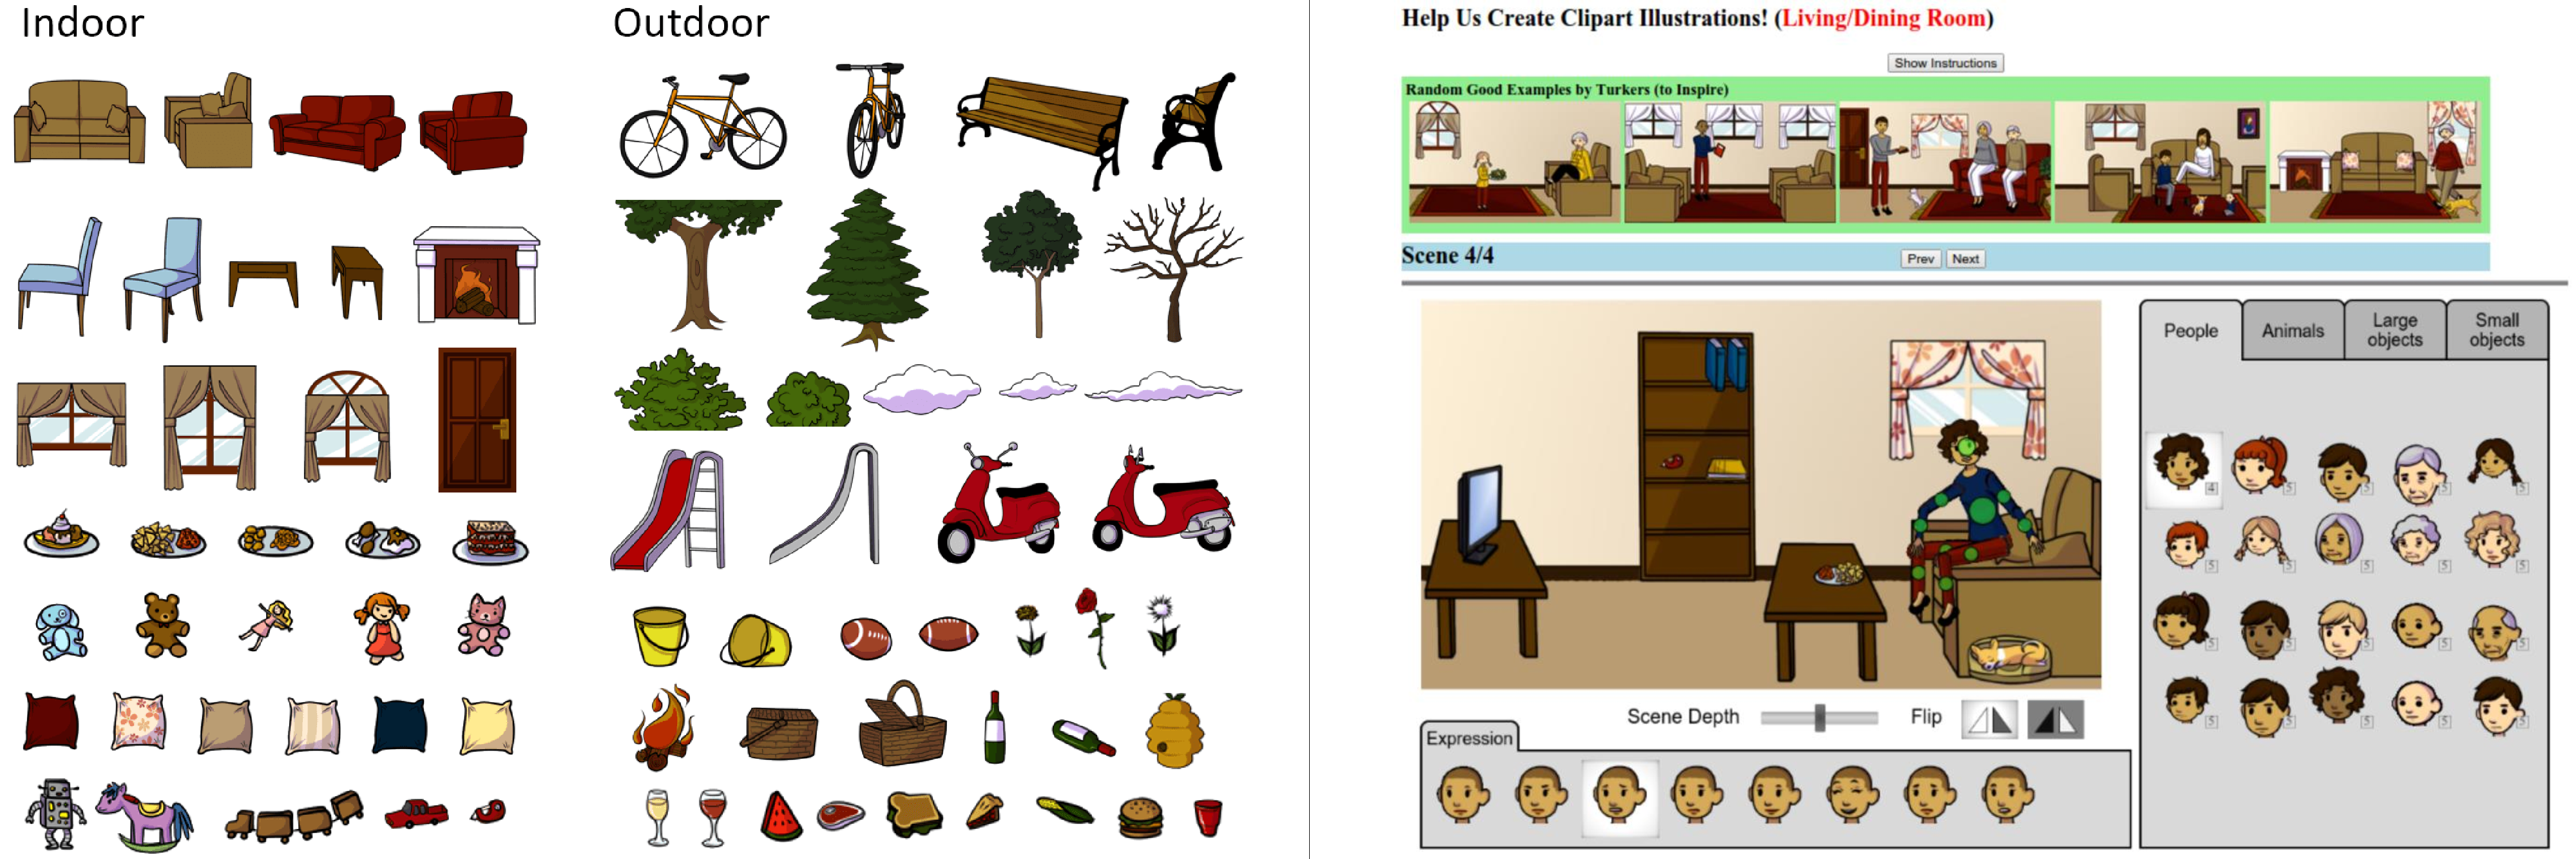
\includegraphics[width=1\linewidth]{figures/clipart_details.pdf}
\caption{Left: A small subset of the objects present in the abstract scene dataset. Right: The AMT interface for collecting abstract scenes.
The light green circles indicate where users can select to manipulate a person's pose. Different objects may be added to the scene using the folders to the right.}
\label{fig:clipart_details}
%\setlength{\belowcaptionskip}{-10pt}
\vspace{10pt}
\end{figure*}

%\begin{figure}[h!]
%\centering
%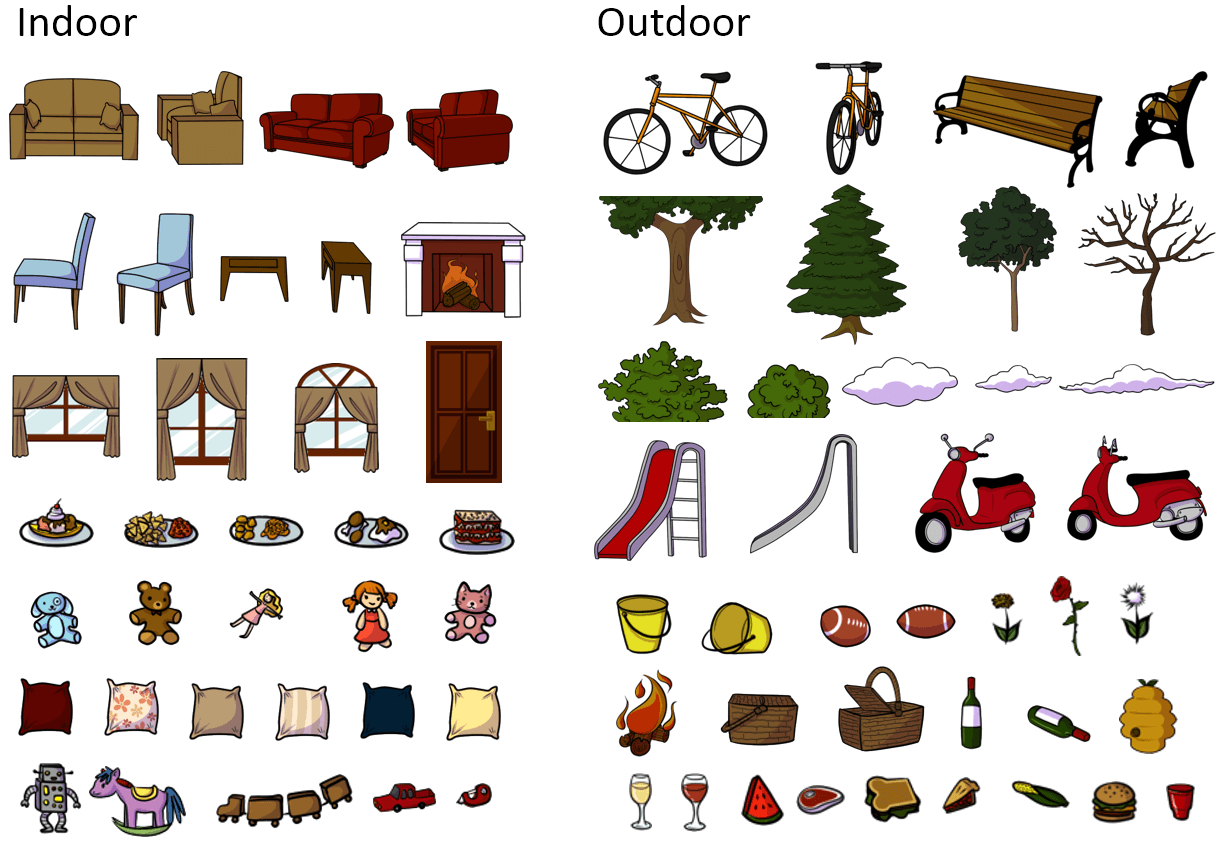
\includegraphics[width=1\linewidth]{figures/objects_min.png}
%\caption{A small subset of the objects present in the abstract scene dataset.}
%%\vspace{-5pt}
%\label{fig:abstractobjects}
%%\setlength{\belowcaptionskip}{-10pt}
%\end{figure}

%\begin{figure}[h!]
%\centering
%\includegraphics[width=1\linewidth]{figures/clipart_interface.pdf}
%\caption{The AMT interface for collecting abstract scenes.
%The light green circles indicate where users can select to manipulate a person's pose. Different objects may be added to the scene using the folders to the right.}
%%\vspace{-5pt}
%\label{fig:abstract}
%%\setlength{\belowcaptionskip}{-10pt}
%\end{figure}
\section*{Appendix VII: User Interfaces}
\label{sec:uis}
In \figref{fig:qstage03}, we show the AMT interface that we used to collect questions for images. Note that we tell the workers that the robot already knows the answer to the previously asked question(s), inspiring them to ask different kinds of questions, thereby increasing the diversity of our dataset.

\figref{fig:answimage} shows the AMT interface used for collecting answers to the previously collected questions when subjects were shown the corresponding images. \figref{fig:answoimage} shows the interface that was used to collect answers to questions when subjects were not shown the corresponding image (\ie, to help in gathering incorrect, but plausible, answers for the multiple-choice task and to assess how accurately the questions can be answered using common sense knowledge alone).

\begin{figure*}[h]
\centering
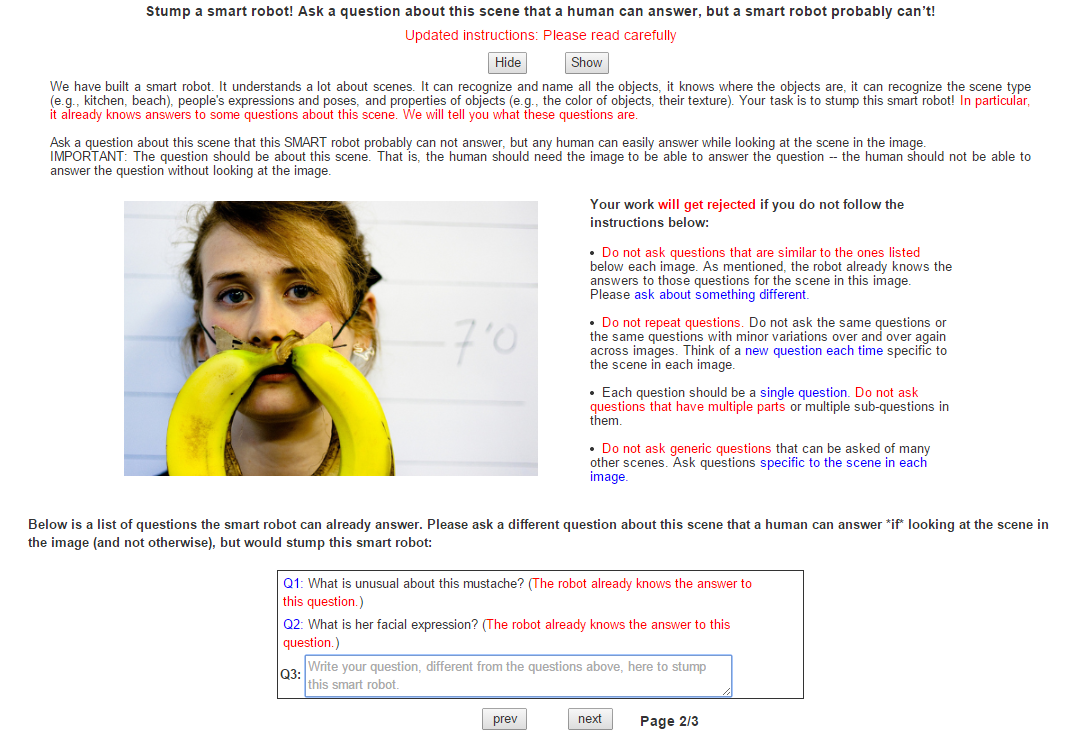
\includegraphics[width=1\linewidth]{figures/question_stage03.png}
\caption{Our AMT interface for collecting the third question for an image, when subjects were shown previous questions that were collected and were asked to ask a question different from previous questions.}
%\vspace{-5pt}
\label{fig:qstage03}
%\setlength{\belowcaptionskip}{-10pt}
\end{figure*}

\begin{figure*}[h]
\centering
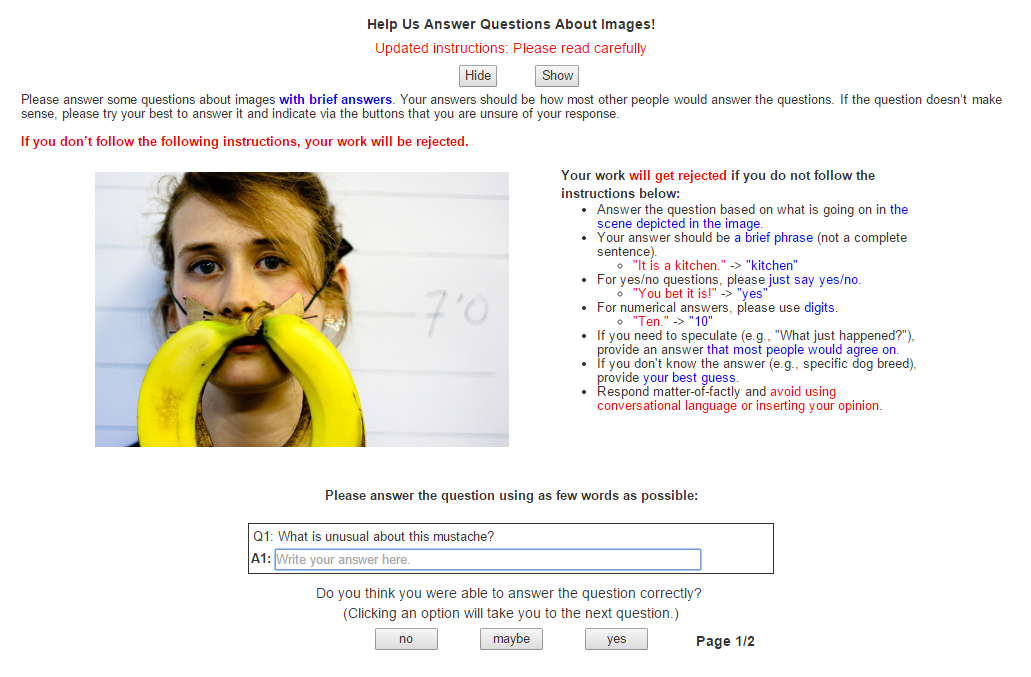
\includegraphics[width=1\linewidth]{figures/answer_with_image.png}
\caption{The AMT interface used to collect answers to a question when subjects were shown the image while answering the question.}
%\vspace{-5pt}
\label{fig:answimage}
%\setlength{\belowcaptionskip}{-10pt}
\end{figure*}

\begin{figure*}[h]
\centering
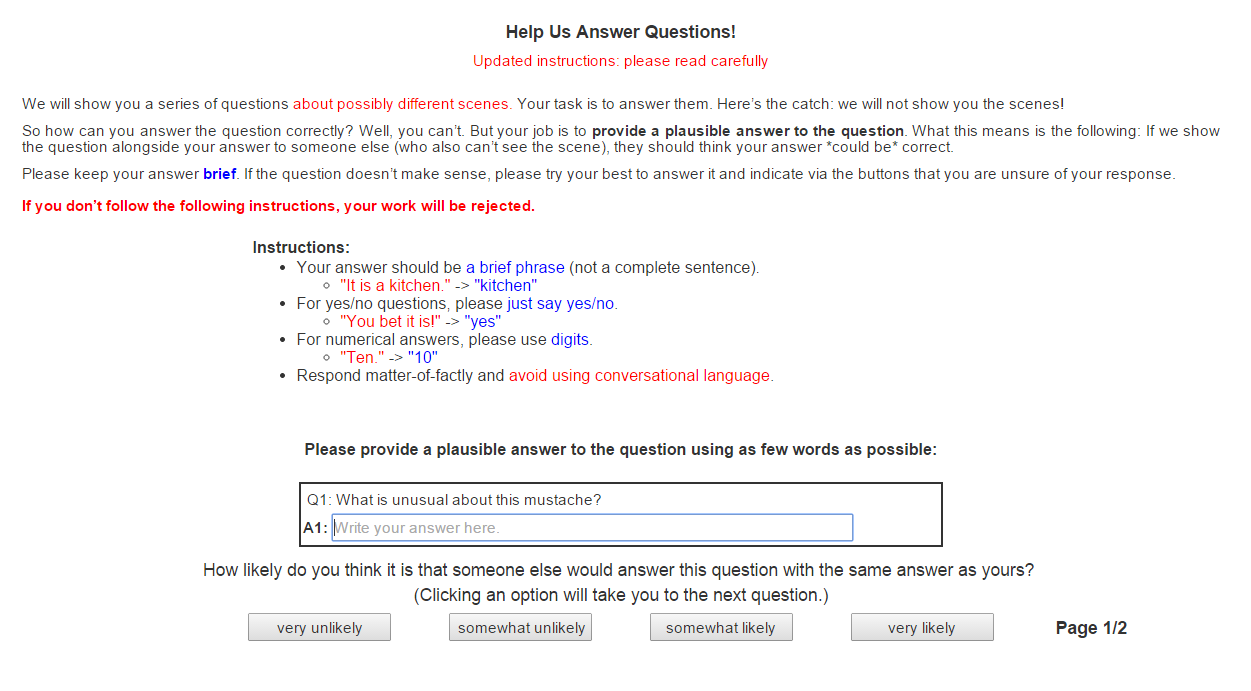
\includegraphics[width=1\linewidth]{figures/answer_without_image.png}
\caption{The AMT interface used to collect answers to a question when subjects were not shown the image while answering the question using only commonsense to collect the plausible, but incorrect, multiple-choice answers.}
%\vspace{-5pt}
\label{fig:answoimage}
%\setlength{\belowcaptionskip}{-10pt}
\end{figure*}
\clearpage

%\vspace{100pt}
\section*{Appendix VIII: Answer Distribution}
\label{sec:top_ans}
\vspace*{-8cm}
The top $250$ answers in our \change{real images} dataset along with their counts and percentage counts are given below. The answers have been presented in different colors to show the different Part-of-Speech (POS) tagging of the answers with the following color code: {\textcolor{magenta}{yes/no}}, {\textcolor{green}{noun}}, {\textcolor{blue}{verb}}, {\textcolor{yellow}{adjective}}, {\textcolor{cyan}{adverb}}, and {\textcolor{red}{numeral}}.

{\textcolor{magenta}{``yes''}} (566613, 22.82\%), {\textcolor{magenta}{``no''}} (381307, 15.35\%), {\textcolor{red}{``2''}} (80031, 3.22\%), {\textcolor{red}{``1''}} (46537, 1.87\%), {\textcolor{yellow}{``white''}} (41753, 1.68\%), {\textcolor{red}{``3''}} (41334, 1.66\%), {\textcolor{yellow}{``red''}} (33834, 1.36\%), {\textcolor{yellow}{``blue''}} (28881, 1.16\%), {\textcolor{red}{``4''}} (27174, 1.09\%), {\textcolor{yellow}{``green''}} (22453, 0.9\%), {\textcolor{yellow}{``black''}} (21852, 0.88\%), {\textcolor{yellow}{``yellow''}} (17312, 0.7\%), {\textcolor{yellow}{``brown''}} (14488, 0.58\%), {\textcolor{red}{``5''}} (14373, 0.58\%), {\textcolor{green}{``tennis''}} (10941, 0.44\%),{\textcolor{green}{``baseball''}} (10299, 0.41\%), {\textcolor{red}{``6''}} (10103, 0.41\%), {\textcolor{green}{``orange''}} (9136, 0.37\%), {\textcolor{red}{``0''}} (8812, 0.35\%), {\textcolor{green}{``bathroom''}} (8473, 0.34\%), {\textcolor{green}{``wood''}} (8219, 0.33\%), {\textcolor{cyan}{``right''}} (8209, 0.33\%), {\textcolor{cyan}{``left''}} (8058, 0.32\%), {\textcolor{green}{``frisbee''}} (7671, 0.31\%), {\textcolor{yellow}{``pink''}} (7519, 0.3\%), {\textcolor{yellow}{``gray''}} (7385, 0.3\%), {\textcolor{green}{``pizza''}} (6892, 0.28\%), {\textcolor{red}{``7''}} (6005, 0.24\%), {\textcolor{green}{``kitchen''}} (5926, 0.24\%), {\textcolor{red}{``8''}} (5592, 0.23\%), {\textcolor{green}{``cat''}} (5514, 0.22\%), {\textcolor{green}{``skiing''}} (5189, 0.21\%), {\textcolor{blue}{``skateboarding''}} (5122, 0.21\%), {\textcolor{green}{``dog''}} (5092, 0.21\%), {\textcolor{green}{``snow''}} (4867, 0.2\%), {\textcolor{yellow}{``black and white''}} (4852, 0.2\%), {\textcolor{green}{``skateboard''}} (4697, 0.19\%), {\textcolor{blue}{``surfing''}} (4544, 0.18\%), {\textcolor{green}{``water''}} (4513, 0.18\%), {\textcolor{green}{``giraffe''}} (4027, 0.16\%), {\textcolor{green}{``grass''}} (3979, 0.16\%), {\textcolor{green}{``surfboard''}} (3934, 0.16\%), {\textcolor{green}{``wii''}} (3898, 0.16\%), {\textcolor{green}{``kite''}} (3852, 0.16\%), {\textcolor{red}{``10''}} (3756, 0.15\%), {\textcolor{yellow}{``purple''}} (3722, 0.15\%), {\textcolor{green}{``elephant''}} (3646, 0.15\%), {\textcolor{green}{``broccoli''}} (3604, 0.15\%), {\textcolor{green}{``man''}} (3590, 0.14\%), {\textcolor{green}{``winter''}} (3490, 0.14\%), {\textcolor{green}{``stop''}} (3413, 0.14\%), {\textcolor{green}{``train''}} (3226, 0.13\%), {\textcolor{red}{``9''}} (3217, 0.13\%), {\textcolor{green}{``apple''}} (3189, 0.13\%), {\textcolor{green}{``silver''}} (3186, 0.13\%), {\textcolor{green}{``horse''}} (3159, 0.13\%), {\textcolor{green}{``banana''}} (3151, 0.13\%), {\textcolor{green}{``umbrella''}} (3139, 0.13\%), {\textcolor{blue}{``eating''}} (3117, 0.13\%), {\textcolor{green}{``sheep''}} (2927, 0.12\%), {\textcolor{green}{``bear''}} (2803, 0.11\%), {\textcolor{green}{``phone''}} (2772, 0.11\%), {\textcolor{red}{``12''}} (2633, 0.11\%), {\textcolor{green}{``motorcycle''}} (2608, 0.11\%), {\textcolor{green}{``cake''}} (2602, 0.1\%), {\textcolor{green}{``wine''}} (2574, 0.1\%), {\textcolor{green}{``beach''}} (2536, 0.1\%), {\textcolor{green}{``soccer''}} (2504, 0.1\%), {\textcolor{yellow}{``sunny''}} (2475, 0.1\%), {\textcolor{green}{``zebra''}} (2403, 0.1\%), {\textcolor{yellow}{``tan''}} (2402, 0.1\%), {\textcolor{green}{``brick''}} (2395, 0.1\%), {\textcolor{green}{``female''}} (2372, 0.1\%), {\textcolor{green}{``bananas''}} (2350, 0.09\%), {\textcolor{green}{``table''}} (2331, 0.09\%), {\textcolor{green}{``laptop''}} (2316, 0.09\%), {\textcolor{green}{``hat''}} (2277, 0.09\%), {\textcolor{green}{``bench''}} (2259, 0.09\%), {\textcolor{green}{``flowers''}} (2219, 0.09\%), {\textcolor{green}{``woman''}} (2197, 0.09\%), {\textcolor{green}{``male''}} (2170, 0.09\%), {\textcolor{green}{``cow''}} (2084, 0.08\%), {\textcolor{green}{``food''}} (2083, 0.08\%), {\textcolor{green}{``living room''}} (2022, 0.08\%), {\textcolor{green}{``bus''}} (2011, 0.08\%), {\textcolor{green}{``snowboarding''}} (1990, 0.08\%), {\textcolor{green}{``kites''}} (1979, 0.08\%), {\textcolor{green}{``cell phone''}} (1943, 0.08\%), {\textcolor{green}{``helmet''}} (1885, 0.08\%), {\textcolor{cyan}{``maybe''}} (1853, 0.07\%), {\textcolor{cyan}{``outside''}} (1846, 0.07\%), {\textcolor{green}{``hot dog''}} (1809, 0.07\%), {\textcolor{green}{``night''}} (1805, 0.07\%), {\textcolor{green}{``trees''}} (1785, 0.07\%), {\textcolor{red}{``11''}} (1753, 0.07\%), {\textcolor{green}{``bird''}} (1739, 0.07\%), {\textcolor{cyan}{``down''}} (1732, 0.07\%), {\textcolor{green}{``bed''}} (1587, 0.06\%), {\textcolor{green}{``camera''}} (1560, 0.06\%), {\textcolor{green}{``tree''}} (1547, 0.06\%), {\textcolor{green}{``christmas''}} (1544, 0.06\%), {\textcolor{green}{``fence''}} (1543, 0.06\%), {\textcolor{green}{``nothing''}} (1538, 0.06\%), {\textcolor{yellow}{``unknown''}} (1532, 0.06\%), {\textcolor{green}{``tennis racket''}} (1525, 0.06\%), {\textcolor{yellow}{``red and white''}} (1518, 0.06\%), {\textcolor{green}{``bedroom''}} (1500, 0.06\%), {\textcolor{green}{``bat''}} (1494, 0.06\%), {\textcolor{green}{``glasses''}} (1491, 0.06\%), {\textcolor{green}{``tile''}} (1487, 0.06\%), {\textcolor{green}{``metal''}} (1470, 0.06\%), {\textcolor{yellow}{``blue and white''}} (1440, 0.06\%), {\textcolor{green}{``fork''}} (1439, 0.06\%), {\textcolor{green}{``plane''}} (1439, 0.06\%), {\textcolor{green}{``airport''}} (1422, 0.06\%), {\textcolor{yellow}{``cloudy''}} (1413, 0.06\%), {\textcolor{red}{``15''}} (1407, 0.06\%), {\textcolor{cyan}{``up''}} (1399, 0.06\%), {\textcolor{yellow}{``blonde''}} (1398, 0.06\%), {\textcolor{green}{``day''}} (1396, 0.06\%), {\textcolor{green}{``teddy bear''}} (1386, 0.06\%), {\textcolor{green}{``glass''}} (1379, 0.06\%), {\textcolor{red}{``20''}} (1365, 0.05\%), {\textcolor{green}{``beer''}} (1345, 0.05\%), {\textcolor{green}{``car''}} (1331, 0.05\%), {\textcolor{blue}{``sitting''}} (1328, 0.05\%), {\textcolor{green}{``boat''}} (1326, 0.05\%), {\textcolor{blue}{``standing''}} (1326, 0.05\%), {\textcolor{yellow}{``clear''}} (1318, 0.05\%), {\textcolor{red}{``13''}} (1318, 0.05\%), {\textcolor{green}{``nike''}} (1293, 0.05\%), {\textcolor{green}{``sand''}} (1282, 0.05\%), {\textcolor{yellow}{``open''}} (1279, 0.05\%), {\textcolor{green}{``cows''}} (1271, 0.05\%), {\textcolor{green}{``bike''}} (1267, 0.05\%), {\textcolor{green}{``chocolate''}} (1266, 0.05\%), {\textcolor{green}{``donut''}} (1263, 0.05\%), {\textcolor{green}{``airplane''}} (1247, 0.05\%), {\textcolor{green}{``birthday''}} (1241, 0.05\%), {\textcolor{green}{``carrots''}} (1239, 0.05\%), {\textcolor{green}{``skis''}} (1220, 0.05\%), {\textcolor{green}{``girl''}} (1220, 0.05\%), {\textcolor{yellow}{``many''}} (1211, 0.05\%), {\textcolor{green}{``zoo''}} (1204, 0.05\%), {\textcolor{green}{``suitcase''}} (1199, 0.05\%), {\textcolor{yellow}{``old''}} (1180, 0.05\%), {\textcolor{green}{``chair''}} (1174, 0.05\%), {\textcolor{yellow}{``beige''}} (1170, 0.05\%), {\textcolor{green}{``ball''}} (1169, 0.05\%), {\textcolor{green}{``ocean''}} (1168, 0.05\%), {\textcolor{green}{``sandwich''}} (1168, 0.05\%), {\textcolor{green}{``tie''}} (1166, 0.05\%), {\textcolor{green}{``horses''}} (1163, 0.05\%), {\textcolor{green}{``palm''}} (1163, 0.05\%), {\textcolor{green}{``stripes''}} (1155, 0.05\%), {\textcolor{green}{``fall''}} (1146, 0.05\%), {\textcolor{green}{``cheese''}} (1142, 0.05\%), {\textcolor{green}{``scissors''}} (1134, 0.05\%), {\textcolor{green}{``round''}} (1125, 0.05\%), {\textcolor{yellow}{``chinese''}} (1123, 0.05\%), {\textcolor{green}{``knife''}} (1120, 0.05\%), {\textcolor{red}{``14''}} (1110, 0.04\%), {\textcolor{green}{``toilet''}} (1099, 0.04\%), {\textcolor{blue}{``don't know''}} (1085, 0.04\%), {\textcolor{green}{``snowboard''}} (1083, 0.04\%), {\textcolor{green}{``truck''}} (1076, 0.04\%), {\textcolor{green}{``boy''}} (1070, 0.04\%), {\textcolor{green}{``coffee''}} (1070, 0.04\%), {\textcolor{yellow}{``cold''}} (1064, 0.04\%), {\textcolor{green}{``fruit''}} (1064, 0.04\%), {\textcolor{blue}{``walking''}} (1053, 0.04\%), {\textcolor{green}{``wedding''}} (1051, 0.04\%), {\textcolor{green}{``lot''}} (1050, 0.04\%), {\textcolor{green}{``sunglasses''}} (1047, 0.04\%), {\textcolor{green}{``mountains''}} (1030, 0.04\%), {\textcolor{green}{``wall''}} (1009, 0.04\%), {\textcolor{green}{``elephants''}} (1006, 0.04\%), {\textcolor{green}{``wetsuit''}} (998, 0.04\%), {\textcolor{green}{``square''}} (994, 0.04\%), {\textcolor{green}{``toothbrush''}} (989, 0.04\%), {\textcolor{blue}{``sleeping''}} (986, 0.04\%), {\textcolor{green}{``fire hydrant''}} (977, 0.04\%), {\textcolor{green}{``bicycle''}} (973, 0.04\%), {\textcolor{green}{``overcast''}} (968, 0.04\%), {\textcolor{green}{``donuts''}} (961, 0.04\%), {\textcolor{green}{``plastic''}} (961, 0.04\%), {\textcolor{green}{``breakfast''}} (955, 0.04\%), {\textcolor{green}{``tv''}} (953, 0.04\%), {\textcolor{green}{``paper''}} (952, 0.04\%), {\textcolor{green}{``ground''}} (949, 0.04\%), {\textcolor{yellow}{``asian''}} (938, 0.04\%), {\textcolor{green}{``plaid''}} (936, 0.04\%), {\textcolor{green}{``dirt''}} (933, 0.04\%), {\textcolor{green}{``mirror''}} (928, 0.04\%), {\textcolor{green}{``usa''}} (928, 0.04\%), {\textcolor{green}{``chicken''}} (925, 0.04\%), {\textcolor{green}{``plate''}} (920, 0.04\%), {\textcolor{green}{``clock''}} (912, 0.04\%), {\textcolor{green}{``luggage''}} (908, 0.04\%), {\textcolor{green}{``none''}} (908, 0.04\%), {\textcolor{green}{``street''}} (905, 0.04\%), {\textcolor{cyan}{``on table''}} (904, 0.04\%), {\textcolor{green}{``spoon''}} (899, 0.04\%), {\textcolor{blue}{``cooking''}} (898, 0.04\%), {\textcolor{yellow}{``daytime''}} (896, 0.04\%), {\textcolor{red}{``16''}} (893, 0.04\%), {\textcolor{green}{``africa''}} (890, 0.04\%), {\textcolor{green}{``stone''}} (884, 0.04\%), {\textcolor{yellow}{``not sure''}} (873, 0.04\%), {\textcolor{green}{``window''}} (868, 0.03\%), {\textcolor{green}{``sun''}} (865, 0.03\%), {\textcolor{green}{``gold''}} (860, 0.03\%), {\textcolor{green}{``people''}} (856, 0.03\%), {\textcolor{green}{``racket''}} (847, 0.03\%), {\textcolor{green}{``zebras''}} (845, 0.03\%), {\textcolor{green}{``carrot''}} (841, 0.03\%), {\textcolor{green}{``person''}} (835, 0.03\%), {\textcolor{green}{``fish''}} (835, 0.03\%), {\textcolor{yellow}{``happy''}} (824, 0.03\%), {\textcolor{green}{``circle''}} (822, 0.03\%), {\textcolor{green}{``oranges''}} (817, 0.03\%), {\textcolor{green}{``backpack''}} (812, 0.03\%), {\textcolor{red}{``25''}} (810, 0.03\%), {\textcolor{green}{``leaves''}} (809, 0.03\%), {\textcolor{green}{``watch''}} (804, 0.03\%), {\textcolor{green}{``mountain''}} (800, 0.03\%), {\textcolor{green}{``no one''}} (798, 0.03\%), {\textcolor{green}{``ski poles''}} (792, 0.03\%), {\textcolor{green}{``city''}} (791, 0.03\%), {\textcolor{green}{``couch''}} (790, 0.03\%), {\textcolor{green}{``afternoon''}} (782, 0.03\%), {\textcolor{green}{``jeans''}} (781, 0.03\%), {\textcolor{yellow}{``brown and white''}} (779, 0.03\%), {\textcolor{green}{``summer''}} (774, 0.03\%), {\textcolor{green}{``giraffes''}} (772, 0.03\%), {\textcolor{green}{``computer''}} (771, 0.03\%), {\textcolor{green}{``refrigerator''}} (768, 0.03\%), {\textcolor{green}{``birds''}} (762, 0.03\%), {\textcolor{green}{``child''}} (761, 0.03\%), {\textcolor{green}{``park''}} (759, 0.03\%), {\textcolor{blue}{``flying kite''}} (756, 0.03\%), {\textcolor{green}{``restaurant''}} (747, 0.03\%), {\textcolor{green}{``evening''}} (738, 0.03\%), {\textcolor{green}{``graffiti''}} (736, 0.03\%), {\textcolor{red}{``30''}} (730, 0.03\%), {\textcolor{blue}{``grazing''}} (727, 0.03\%), {\textcolor{green}{``flower''}} (723, 0.03\%), {\textcolor{yellow}{``remote''}} (720, 0.03\%), {\textcolor{green}{``hay''}} (719, 0.03\%), {\textcolor{red}{``50''}} (716, 0.03\%). 


\section*{Appendix IX: Additional Examples}
\label{sec:dataset_stats}

To provide insight into the dataset, we provide additional examples. In \figref{fig:coco_more_examples}, \figref{fig:abstract_more_examples}, and \figref{fig:mc_examples}, we show a random selection of the VQA dataset for the MS COCO~\cite{coco} images, abstract scenes, and multiple-choice questions, respectively.

\begin{figure*}[t]
\centering
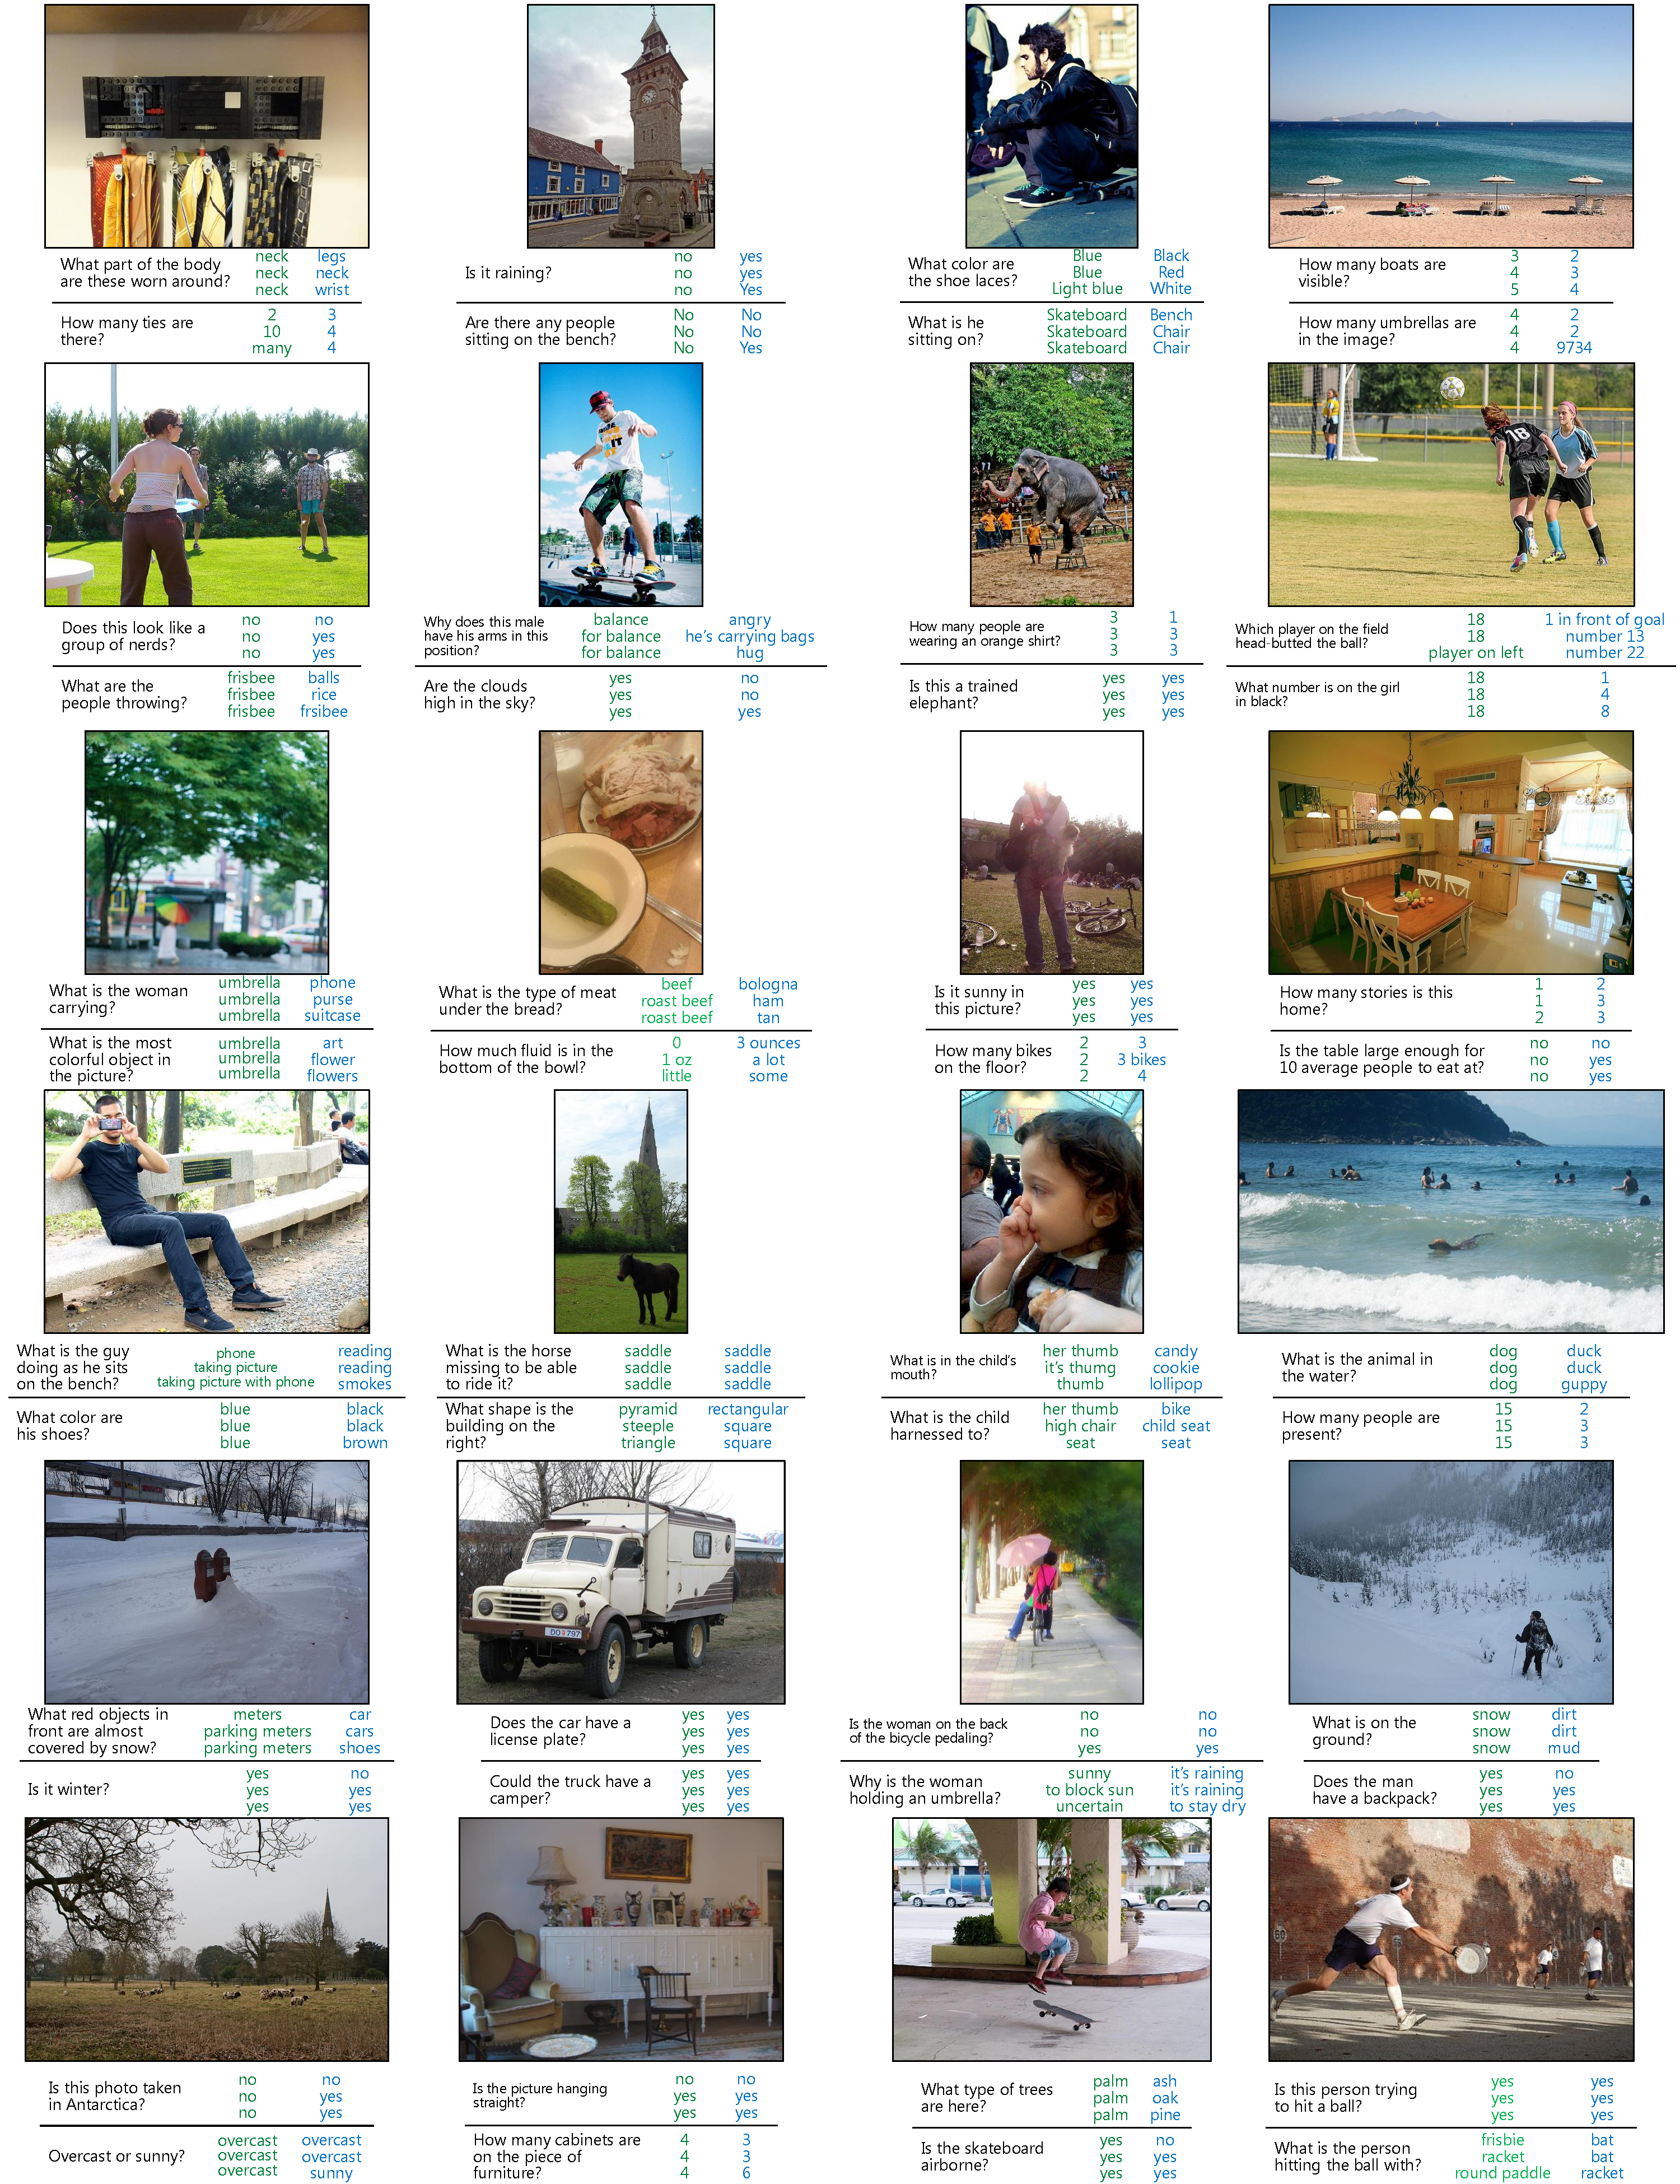
\includegraphics[width=1\linewidth]{figures/coco_examples-compressed.pdf}
\caption{Random examples of questions (black), \change{(a subset of the)} answers given when looking at the image (green), and answers given when not looking at the image (blue) for numerous representative examples of the real image dataset.}
%\vspace{-5pt}
\label{fig:coco_more_examples}
%\setlength{\belowcaptionskip}{-10pt}
\end{figure*}

\begin{figure*}[t]
\centering
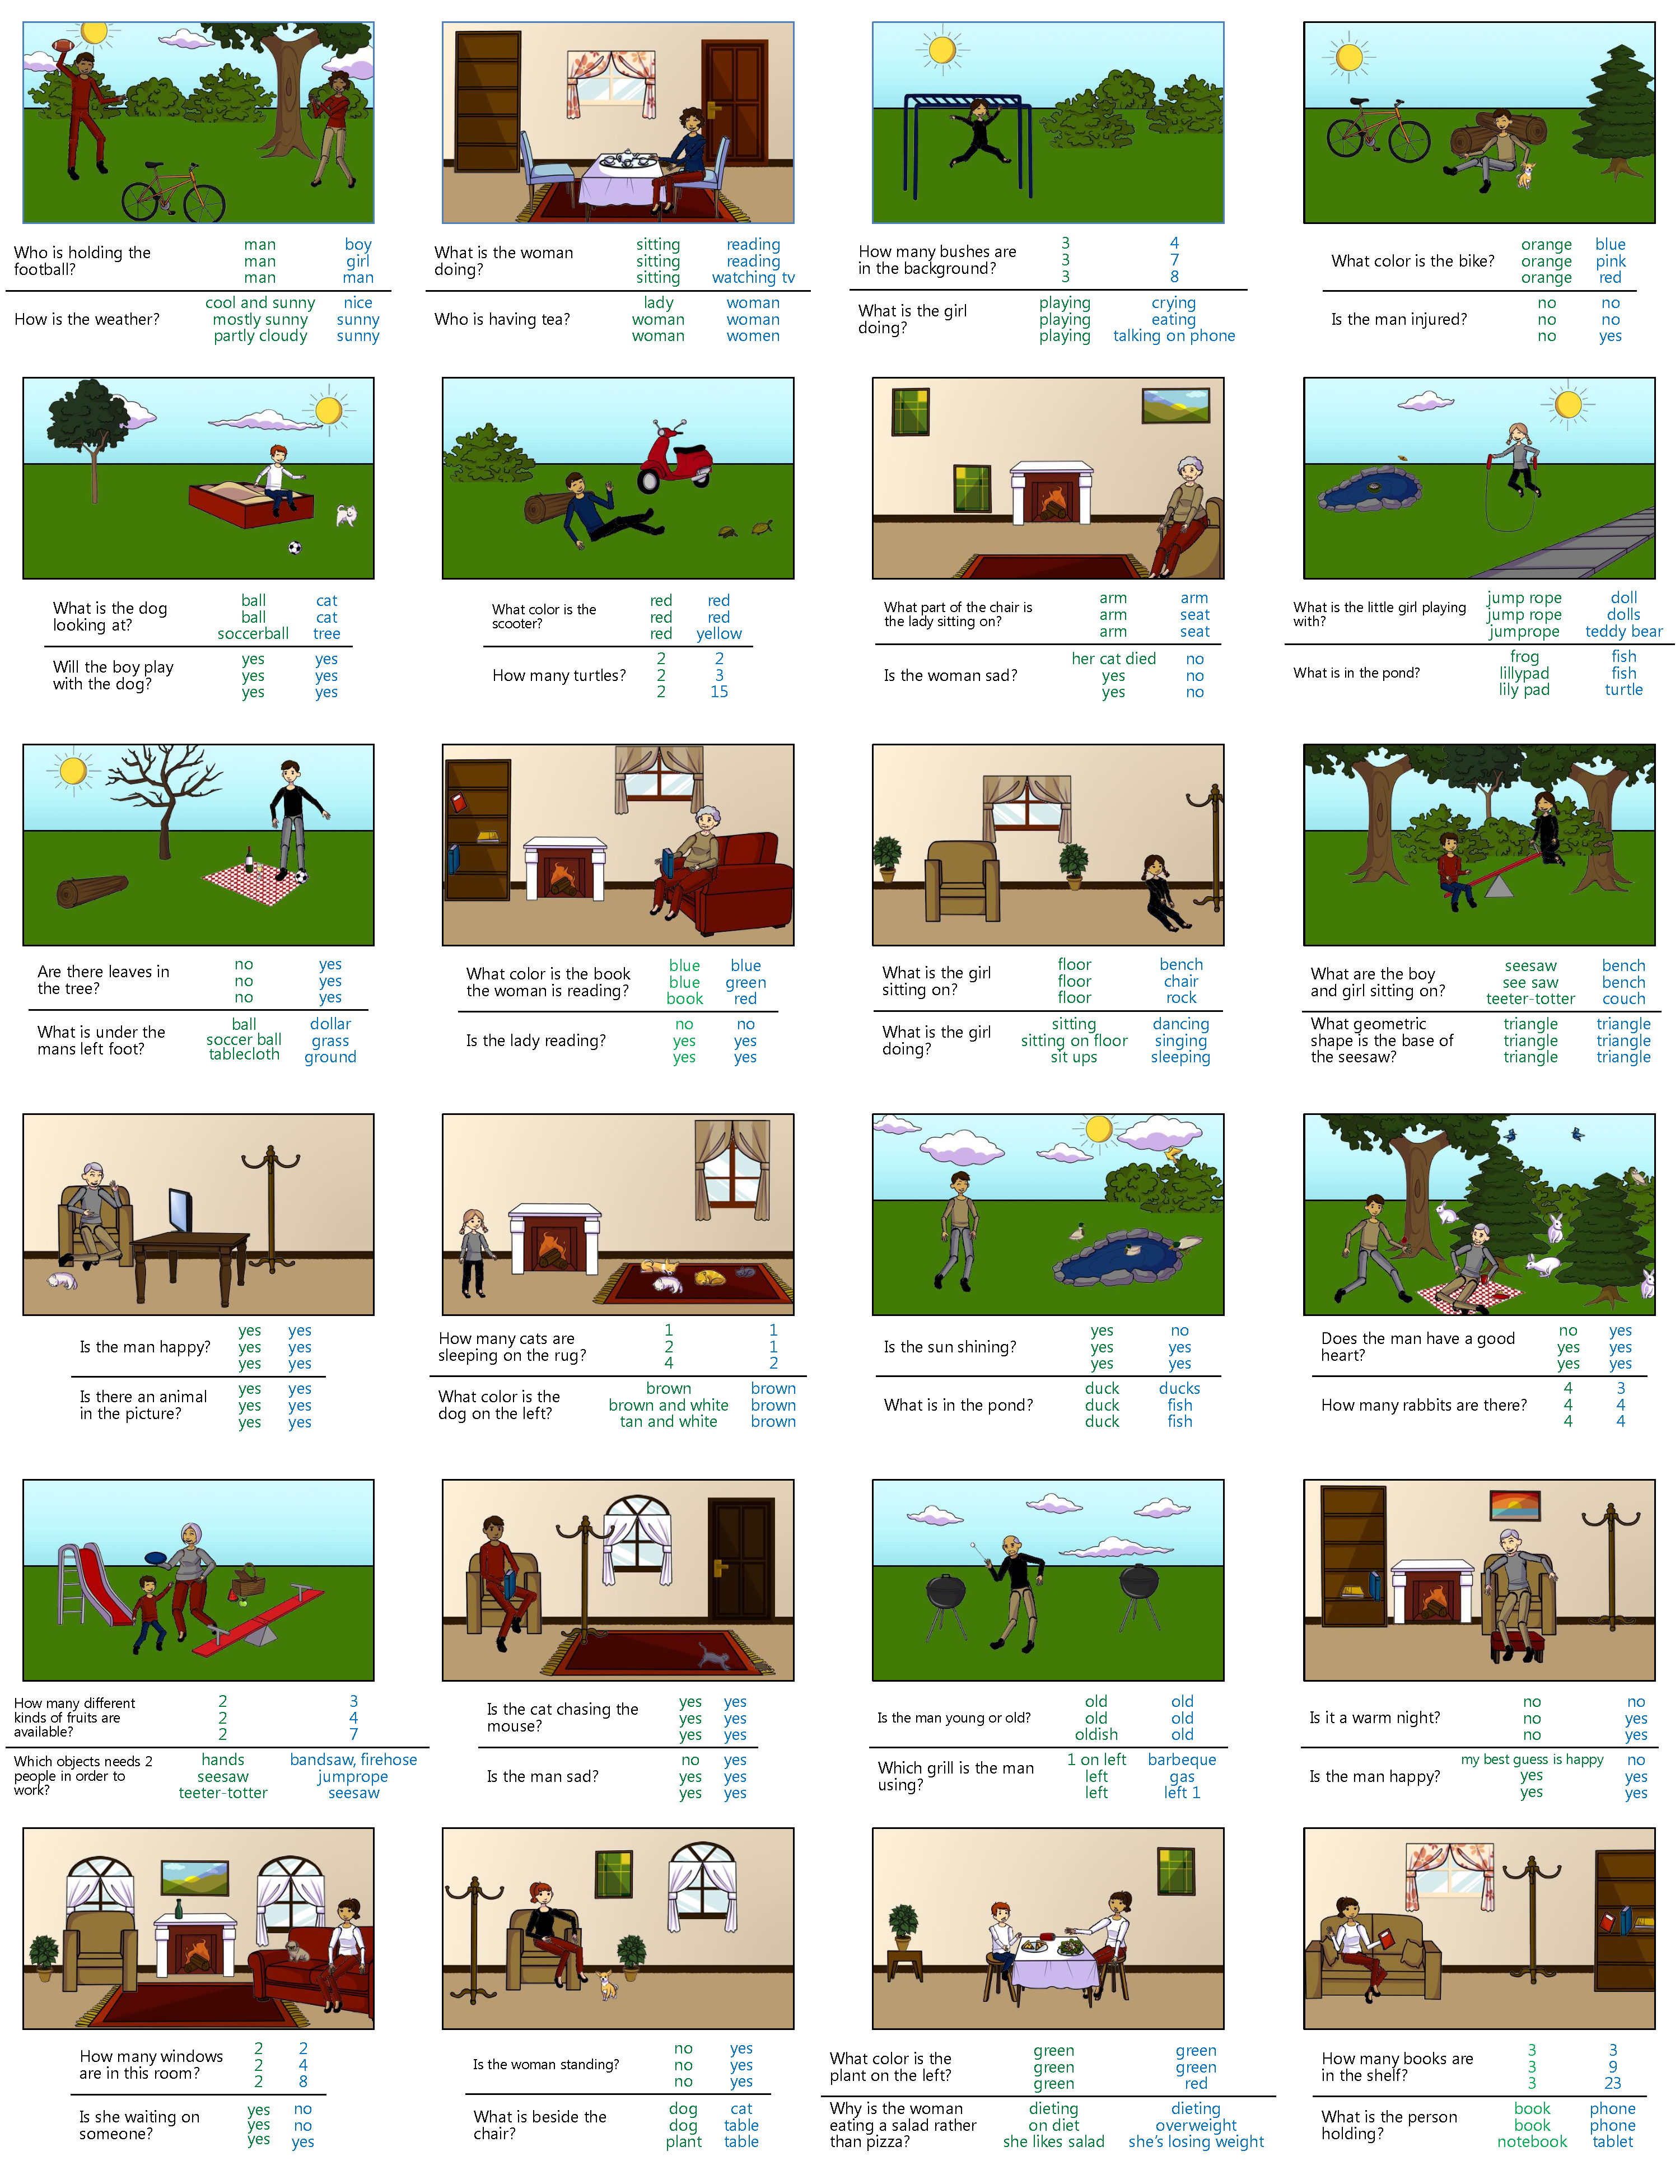
\includegraphics[width=1\linewidth]{figures/abstract_examples-compressed.pdf}
\caption{Random examples of questions (black), \change{(a subset of the)} answers given when looking at the image (green), and answers given when not looking at the image (blue) for numerous representative examples of the abstract scene dataset.}
%\vspace{-5pt}
\label{fig:abstract_more_examples}
%\setlength{\belowcaptionskip}{-10pt}
\end{figure*}

\begin{figure*}[t]
\centering
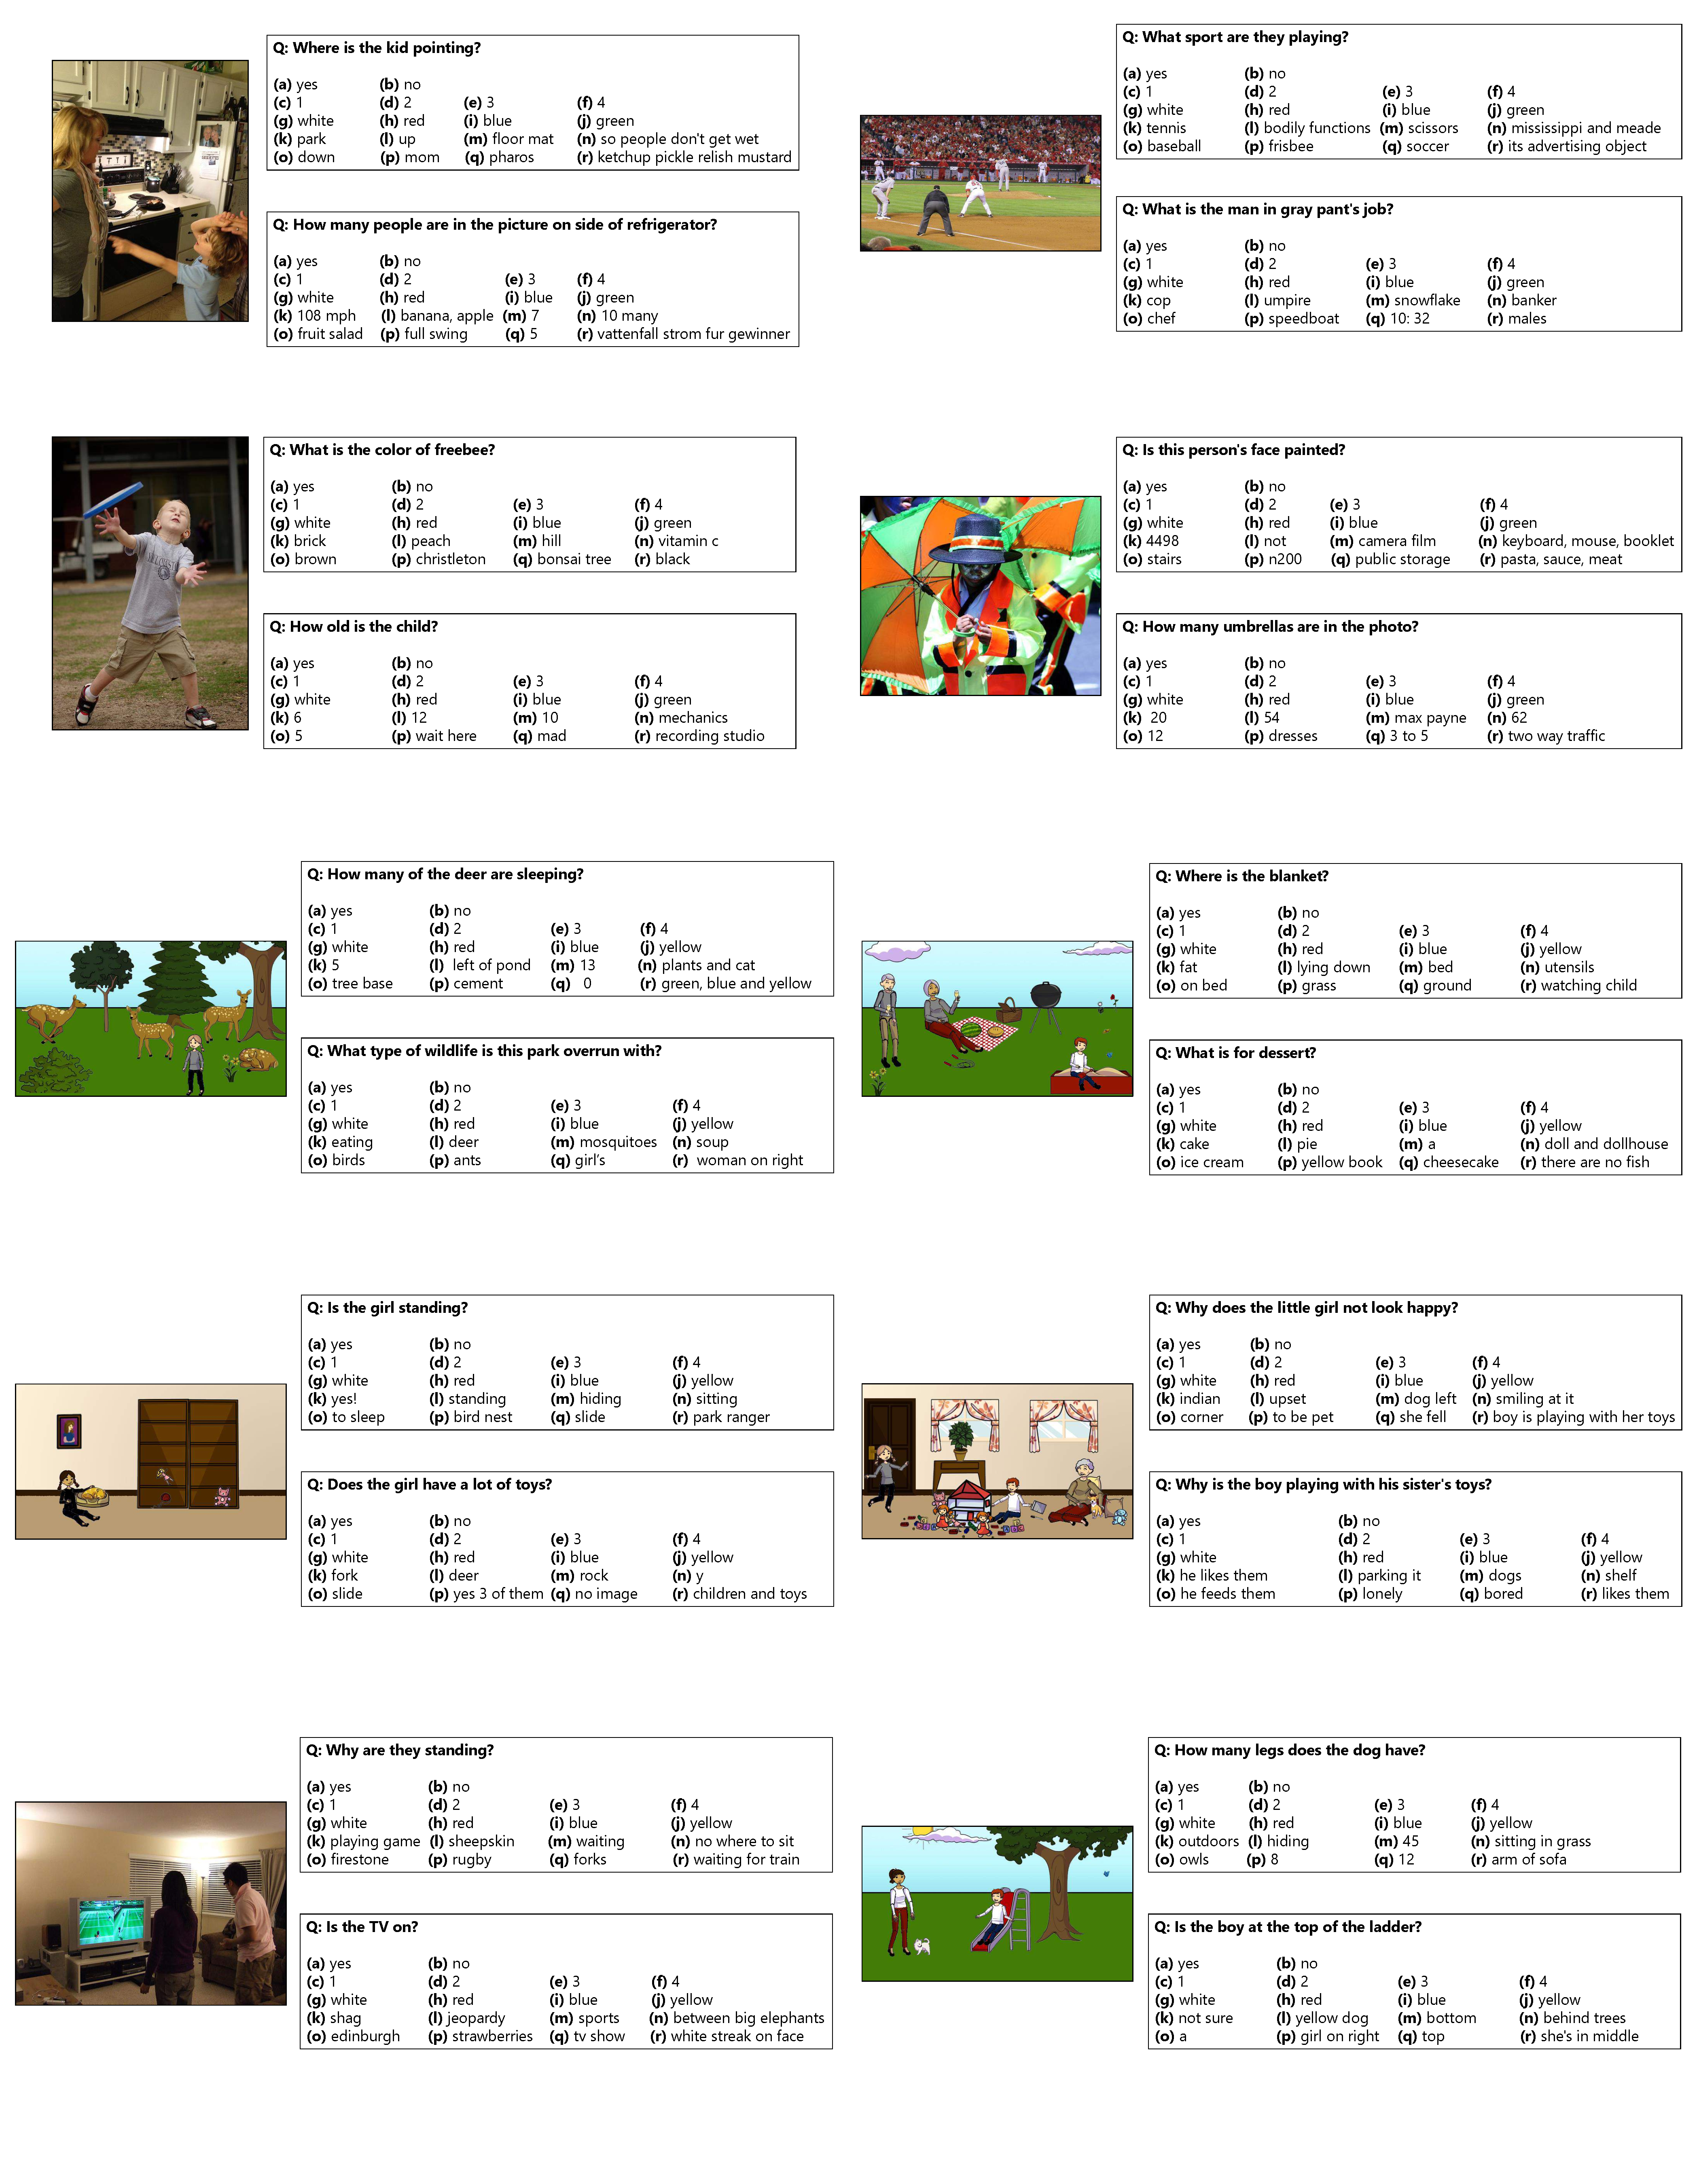
\includegraphics[width=1\linewidth]{figures/MC_examples_compressed.pdf}
\caption{Random examples of multiple-choice questions for numerous representative examples of the real and abstract scene dataset.}
%\vspace{-5pt}
\label{fig:mc_examples}
%\setlength{\belowcaptionskip}{-10pt}
\end{figure*}

%%%%%%%%%%%%%%%%%%%%%%%%%%%%%%%%%%%%%%%%%%%%%%%%%%%%%%%%%%%
% References
%%%%%%%%%%%%%%%%%%%%%%%%%%%%%%%%%%%%%%%%%%%%%%%%%%%%%%%%%%%

\clearpage
{\footnotesize
\bibliographystyle{ieee}
\bibliography{vqa_main}
}

\end{document}
